\documentclass[runningheads,a4paper]{llncs}

\usepackage{latexsym}
\usepackage{setspace}
\usepackage{cancel}
\usepackage{listings}
\usepackage{graphicx}
\usepackage{appendix}
\usepackage{amssymb}
\usepackage{stmaryrd}
\usepackage{amsmath}
\usepackage{leftidx}
\usepackage{mathtools}
\usepackage[linesnumbered,noend]{algorithm2e}
\usepackage{paralist}


%\usepackage{cancel}
%\usepackage{verbatim}
%\usepackage{chngpage}
%\usepackage{fullpage}

\usepackage{color}

\usepackage{mathrsfs}
\usepackage{tikz}
\usetikzlibrary{shapes}
\usepackage{times}
%\usepackage{pslatex}
\newcommand{\hide}[1]{}

\newcommand*\circled[1]{\overline{#1}}

\hide{
\newcommand*\circled[1]{
	\mathchoice
	{\tikz[baseline=(char.base)]{\node[draw,inner sep=0pt, scale=0.75,ellipse,font=\small] (char) {${#1}$};}}
	{\tikz[baseline=(char.base)]{\node[draw,inner sep=0pt, scale=0.75,ellipse,font=\small] (char) {${#1}$};}}
	{\tikz[baseline=(char.base)]{\node[draw,inner sep=0pt, scale=0.75,ellipse,font=\tiny] (char) {${#1}$};}}
	{\tikz[baseline=(char.base)]{\node[draw,inner sep=0pt, scale=0.55,ellipse,font=\tiny] (char) {${#1}$};}}
	}}
%\newtheorem{definition}{Definition}
%\newtheorem{theorem}{Theorem}
%\newtheorem{proposition}[theorem]{Proposition}
%\newtheorem{corollary}[theorem]{Corollary}
%\newtheorem{example}{Example}
%\newtheorem{question}{Open Question}
%\newtheorem{lemma}[theorem]{Lemma}
%\newtheorem{Algo}{Algorithm}
%\newtheorem{remark}[theorem]{Remark}

\def\arr#1{\stackrel{#1}{\longrightarrow}}

\def\Aa{{\mathcal{A} }}

\def\Bb{{\mathscr{B} }}

\def\Cc{{\mathcal{C} }}

\def\Dd{{\mathbb{D} }}

\def\Ee{{\mathcal{E} }}

\def\Ff{{\mathcal{F} }}

\def\Zz{{\mathcal{Z} }}

\def\Nn{{\mathbb{N} }}

\def\Ss{{\mathcal{S} }}

\def\schm{{\mathfrak{s} }}

\def\Tt{{\mathcal{T} }}

\def\Ii{{\mathbb{Z} }}

\def\Jj{{\mathcal{J}}}

\def\Vv{{\mathcal{V}}}

\def\Rr{{\mathcal{R} }}

\def\Ll{{\mathcal{L}}}

\def\Kk{{\mathcal{K}}}


\def\treeset{{\mathscr{T}}}

\def\contextset{{\mathcal{C}}}

\def\theory{{\mathcal{L}}}

\def\termset{{\mathcal{T}}}

\def\formulaset{{\mathcal{F}}}

\newcommand\univ{\mathsf{Univ}}

\newcommand\op{\mathfrak{o}}

\newcommand\dv{\mathtt{x}}

\newcommand\ydv{\mathtt{y}}

\newcommand\cv{\mathtt{z}}

\newcommand\thla{\mathcal{LIA}}

\newcommand\thdif{\mathcal{DIF}}

\newcommand\thord{\mathcal{ORD}}

\newcommand\thset{\mathcal{SET}}

\newcommand\thmset{\mathcal{MUS}}

\newcommand\natnum{{\mathbb{N} }}

\newcommand\intnum{{\mathbb{Z} }}

\newcommand\cur{\mathsf{cur}}
\newcommand\nnext{\mathsf{next}}
\newcommand\head{\mathsf{hd}}
\newcommand\tail{\mathsf{tl}}
\newcommand\init{\mathsf{init}}

\newcommand{\loopL}[1]{\mbox{loop\{} #1\mbox{\}}}
\newcommand{\ite}[3]{\mbox{if } #1 \mbox{ then } #2\mbox{ else }#3 }



\newcommand\vars{\mathsf{vars}}

\newcommand\intvars{\mathcal{X}}

\newcommand\dom{\mathsf{dom}}

\newcommand\rng{\mathsf{rng}}

\newcommand\ltrue{\mathsf{true}}

\newcommand\lfalse{\mathsf{false}}

\newcommand\avg{\mathrm{avg}}

\newcommand\maxv{\mathsf{max}}

\newcommand\sumv{\mathsf{sum}}

\newcommand\cntv{\mathsf{cnt}}

\newcommand\addeq{+\!\!=}

\newcommand\defval{\mathsf{DEF}}

%\newcommand{\sub}[2]{\mathsf{sub}_{#2}(#1)}
\newcommand{\eval}[2]{\llbracket#1\rrbracket_{#2}}

%%%%%%%%%%%%%%%%%%%%%%%%%%%%%%%%%%%%%%%%%%%%
%%%%%%%%%%%The macros introduced by Zhilin%%%%%%%%%%%%%
%%%%%%%%%%%%%%%%%%%%%%%%%%%%%%%%%%%%%%%%%%%%
\newcommand{\sval}{\Omega}
\newcommand{\sumf}{\Theta}
\newcommand{\initval}{\sval}

% The macros for the data variables.
\newcommand{\vard}{\mathfrak{d}}
\newcommand{\vare}{\mathfrak{e}}
\newcommand{\varf}{\mathfrak{f}}
\newcommand{\varo}{\mathfrak{o}}
\newcommand{\varx}{\mathfrak{x}}
\newcommand{\vary}{\mathfrak{y}}

% The macros for the data variables.
\newcommand{\csta}{\alpha}
\newcommand{\cstb}{\beta}
\newcommand{\cstg}{\gamma}
\newcommand{\cste}{\varepsilon}
\newcommand{\cstl}{\lambda}
\newcommand{\cstm}{\mu}
\newcommand{\cstn}{\nu}


\newcommand{\gmlasso}{\mathfrak{m}}
%%%%%%%%%%%%%%%%%%%%%%%%%%%%%%%%
%%%%%%%%%%%%%%%%%%%%%%%%%%%%%%%%
%%%%%%%%%%%%%%%%%%%%%%%%%%%%%%%%

\newcommand{\abs}{\mathsf{Abs}}

<<<<<<< HEAD
\newcommand{\cabs}{\mathscr{F}}

\newcommand{\sntcset}{\mathscr{C}}

\newcommand{\sntc}{\mathsf{cl}}


\newcommand{\hide}[1]{}
=======

>>>>>>> 23ee7d3e193b8d535dc2f03697e699e887154d31
\newcommand{\yfc}[1]{\color{blue} {YF: #1 :FY} \color{black}}
\newcommand{\zhilin}[1]{\color{cyan} {ZL: #1 :LZ} \color{black}}
\newcommand{\lei}[1]{\color{green} {LE: #1 :EL} \color{black}}
\newcommand{\SDSIT}{SDSIT}
\newcommand{\Name}{Streaming data string to integer transducer}
\newcommand{\name}{streaming data string to integer transducer}
\newcommand{\interval}[1]{[#1]}
%\def\Ss{{$\mathcal{A}$\ }}

\title{The~Commutativity~Problem~of~the~MapReduce Framework: A Transducer-based Approach}
\titlerunning{Commutativity of MapReduce: A Transducer-based Approach}
\author{}
\institute{}

%\author{Yu-Fang Chen, Lei Song, Zhilin Wu}

\begin{document}

\maketitle

\begin{abstract}

MapReduce is a popular programming model for data parallel computations. 
In MapReduce, the \emph{reducer} produces an output from a list of inputs. Due to the scheduling policy of the platform, the inputs may arrive at the reducers in different order. The \emph{commutativity problem} of reducers asks if the output of a reducer is independent of the order of its inputs. Although the problem is undecidable in general,
%due to Rice's theorem and thus is seemingly uninteresting. 
the MapReduce programs in practice are usually used for data analytics and thus require very simple data and control flow. 
By exploiting the simplicity, we propose a programming language for reducers where the commutativity problem is decidable.
 %The programming language is capable of modeling many daily tasks in practice, e.g. the aggregate functions $sum$, $max$, $min$, $count$, the filters like $age \ge 18$, as well as their compositions. 
The decision procedure is obtained through a reduction to the equivalence problem of \emph{streaming numerical transducers} (SNTs), a novel automata model over infinite alphabets introduced in this paper. The design of SNTs is inspired by streaming transducers (Alur and Cerny, POPL 2011). Nevertheless, the two models are intrinsically different since the outputs of SNTs are integers while those of streaming transducers are data strings. 
%The main ingredients of SNTs are to divide the set of variables into the set of control variables and data variables where the control variables can be used in the guards of transitions, but without arithmetics, on the other hand, the data variables are allowed to be updated with arithmetics, but they are forbidden to occur in the guards. 
The decidability of the equivalence of SNTs is achieved with an involved combinatorial analysis of the evolvement of the values of the integer variables during the runs of SNTs.
%We show that the language is expressive enough for common data analytics operations.
\end{abstract}

%!TEX root = main-cav.tex

\section{Introduction}
%What is Map-Reduce
MapReduce is a  popular framework for data parallel computations. It has been adopt in various cloud computing frameworks such as Hadoop~\cite{Hadoop} and Spark~\cite{Spark}. In a typical MapReduce program, a \emph{mapper} reads from data sources and outputs a list of key-value pairs. 
The load balance mechanism of the Map-Reduce framework reorganizes the key-value pairs $(k, v_1), (k,v_2)\ldots(k,v_n)$ with the same key $k$ to a pair $(k,l)$, where $l$ is a list of values $v_1,v_2,\ldots,v_n$, and sends $(k,l)$ to a \emph{reducer}. The reducer then iterates through the list and output a key-value pair.

To be more concrete, taking the ``word-counting'' MapReduce program as an example. It counts the occurrences of each word in a set of documents. The mappers read the documents and output for each document a list in the form of $(word_1, count_1), (word_2, count_2), \ldots, (word_n, count_n)$, where $count_k$ is the number of occurrences of $word_k$ in the document being processed. These lists will be reorganized into the form of $(word_1, list_1), (word_2,list_2), \ldots, (word_n,list_n)$ and sent to the reducers, where $list_k$ is a list of integers recording the number of occurrences of $word_k$ in the set of documents. Note that the \emph{order} of the integers in the lists can differ in different executions due to network latency, load balancing, etc.
This results in the \emph{commutativity problem}.

%The communitativity problem and its importance
We say that a reducer is \emph{commutativity} if its output is independent of the order of its inputs. The commutativity problem asks if a reducer is commutativity. A study from Microsoft~\cite{XZZ+14} reports that 58\% of the 507 reducers submit to their MapReduce platform are non-commutative, which may lead to very tricky and hard-to-find bugs.
As an evidence, those reducers already went through serious code review, testing, and experiments with real data for more than three months. Still, among them 5 reducers containing very subtle bugs caused by non-commutativity (confirmed by the programmers). 
Moreover, having the commutativity property makes reproducing a bug found by program testing easier.

%The reason for studying syntatical restrictions 
The reducer commutative problem in general is undecidable by Rice's theorem. However, in practice, the reducers are seldom Turing machines. They are usually used for data analytics and have very simple control structures. Many of them just iterate through the input list and compute the output with very simple operations.
We want to study if the commutative problem of real-world reducers are decidable.

%The tacas 2015 undecidability result
A simple programming language of reducers over integers has been considered in~\cite{CHSW15}, where the only loop structure allowed is an iteration over the input list and it is not allowed to reset the iterator to the list head. They show that the commutative problem of programs written by such a simple language is undecidable by a reduction from the satisfiability problem of Diophantine equations. Under scrutiny, we found that the language is still too expressive for typical data analytics programs. For example, it allows arbitrary multiplications of variables, which is a key element in the undecidability proof. 

%our languge
By observing the behavioral pattern of reducer programs for data analytics, we characterize the essential components in a programming language for reducers. %However, we found that even only with the essential parts of the language, the commutativity problem is still undecidable. 
We found that the commutativity problem becomes decidable if we partition variables into \emph{control variables} and \emph{data variables}. Data variables cannot be used in transition guards and control variables can store only elements in the input list (e.g., it is not allowed to store the sum of two variables in a control variable). 
We believe such concepts provide good insights for reducer programming language design.

%%%SNTs
We define a formalism named \emph{streaming numerical transducers (SNT)} and use it to create a decision procedure for the reducer commutative problem.
The design of SNTs is inspired by the streaming transducer model~\cite{RP11}.
It generalizes register automata~\cite{KF94,NSV04} to allow quantifier-free Presburgh arithmetic over variables and input values, with restrictions on the structure of the transition systems.
We show that the equivalence, commutative, and non-zeroness problems of SNTs are decidable.
Moreover, SNTs can be composed to form a commutative/equivalence proof of reducer programs that read the input list multiple times (Section~\ref{sec_cases}).
The study of SNT is interesting on its own right. As far as we know, this is the \emph{first} automata model over infinite alphabet where quantifier-free Presburgh arithmetics over variables and values from an unbounded input tape are allowed. Moreover, the model can be applied to the verification of other interesting classes of programs, programs with unbounded list as input.

As far as we know, the SNT model  is different from all other automata models. The symbolic transducer~\cite{VHL+12} cannot remember and aggregate input data over different locations. Register automata~\cite{KF94,NSV04} do not allow arithmetics over integers. Cost register automata~\cite{ADD+13} assumes finite alphabet. Streaming transducers~\cite{RP11} does not allow Presburgh arithmetics over values from the input tape.  

The rest of the paper is organized as follows. Section~\ref{sec:preliminaries} defines notations we use in the paper. Section~\ref{sec:language} describes our design of the verifiable programming language for reducers. Section~\ref{sec:def-snt} describes design of the \emph{streaming numerical transducer} (SNT) model, including the formal definition and Section~\ref{sec:dec-snt} describes the decision procedure of SNTs. Sec~\ref{sec:cases} demonstrates how to use our framework to verify the commutativity property over more challenging data analytics programs. We conclude the paper in Section~\ref{sec:conclusion}. 

%!TEX root = main-cav.tex

\section{Preliminaries}
\label{sec:preliminaries}
Let $\intnum$,  $\intnum^+$ be the set of integers, positive integers, respectively and $\bot \not \in \intnum$ be  the undefined value. By convention, it is assumed that $\bot + \bot = \bot$, $\bot + n = \bot$ for each $n \in \intnum$, $0 \times \bot = 0$, and $n \times \bot = \bot$ for each $n \in \intnum^+$.
In this paper, we assume that all variables range over $\intnum \cup \{\bot\}$.  

For a function $\rho$, let $\dom(\rho)$ and $\rng(\rho)$ denote the \emph{domain}  and \emph{range} of $\rho$, respectively. We use $\rho_\bot$ to denote a function with empty domain. An \emph{expression} $e$ over the set of variables $Z$ is defined by the following rules, $e\equiv  c \mid  c z \mid (e + e) \mid (e - e)$, where $z \in Z$ and $c\in \intnum$.  As a result of the commutativity of $+$, without loss of generality, we assume that all expressions $e$ in this paper are of the form $c_0 + c_1 z_1 + \dots c_n z_n$, where $c_0, c_1,\dots,c_n \in \intnum$ and $z_1,\dots,z_n \in Z$. 

% \zhilin{I changed a bit the definition of expressions here} 

For an expression $e$, let $\vars(e)$ denote the set of variables occurring in $e$. Let $\Ee_Z$ denote the set of all expressions over the set of variables $Z$. 
%Let $e$ be an expression and $\eta$ be a partial function from $\vars(e)$ to expressions. Then we use $\sub{e}{\eta}$ to denote the expression obtained from $e$ by replacing each variable $z \in \vars(e)\cap\dom(\eta)$ with $\eta(z)$. 
A \emph{valuation} $\rho$ of $Z$ is a function from $Z$ to $\intnum\cup\{\bot\}$. A \emph{symbolic valuation} $\sval$ of $Z$ is a function which maps each variable $z \in Z$ to an expression (possibly over a different set of variables). The value of $e$ under a valuation $\rho$ (resp. symbolic valuation $\sval$), denoted by $\eval{e}{\rho}$ (resp. $\eval{e}{\sval}$), is defined recursively in the standard way. For example, let $\sval$ be a symbolic valuation the maps $z_1$ to $z_1+z_2$ and $z_2$ to $3z_2$, then $\eval{2z_1+3z_2}{\sval}=2\eval{z_1}{\sval}+3\eval{z_2}{\sval}=2(z_1+z_2)+3(3z_2)=2z_1+11z_2$.
%Note that a valuation can be seen as a special symbolic valuation where the image of each variable is a constant.
For a valuation $\rho$, $z\in Z$, and $d \in \intnum$, define the function $\rho[d/z]$ such that $\rho[d/z](z)=d$ and $\rho[d/z](z')=\rho(z')$ for $z'\neq z$. 

In this paper, we use $X$ and $Y$ to denote the sets of \emph{control variables} and \emph{data variables}, respectively. We use the variable $\cur \notin X\cup Y$ to store the data value that is currently being processed in the input list and use $X^+$ to denote the set $X\cup \{\cur\}$.
A \emph{guard} is a formula defined by the following rules, $g::= \ltrue \mid \cur\odot c \mid \cur\odot x \mid g \wedge g$, where $\odot \in \{=,\neq,<, >, \le, \ge\}$, $x \in X$, and $c\in \intnum$. 
Let $\rho$ be a valuation and $g$ be a guard. Then $\rho$ satisfies $g$, denoted by $\rho \models g$, iff for each variable $z \in \vars(g)$, $\rho(z) \neq \bot$, and $g$ is evaluated to $\ltrue$ under $\rho$. 

Let $\interval{n}$ be the set $\{ 1, 2, \ldots, n \}$. Let $\interval{a,b}$ be the set $\{ a, a+1, \ldots, b \}$ when $b\geq a$ and $\emptyset$ otherwise. A \emph{permutation} on
$\interval{n}$ is a one-to-one and onto mapping from $\interval{n}$ to
$\interval{n}$. The set of
permutations on $\interval{n}$ is denoted by $S_n$.

A \emph{data word $w$} is a sequence of integer values $d_1\ldots d_n$ such that $d_i \in \intnum$ for each $i$.
We use $\head(w)$, $\tail(w)$, and $|w|$ to denote the data value $d_1$, the tail $d_2\dots d_n$, and the length $n$, respectively.
We use $\epsilon$ to denote an empty data word. As a convention, we let $\head(w)=\bot$, $\tail(w)=\epsilon$, and $|w|=0$.
Given two data words $w,w'$, we use $w.w'$ to denote their concatenation.
Given $\sigma \in S_n$, we lift $\sigma$ to data words by defining $\sigma(w)=d_{\sigma(1)} \ldots d_{\sigma(n)}$, for each data word $w=d_1\ldots d_n$. We call $\sigma(w)$ as a permutation of $w$.

%!TEX root = main-cav.tex
 
\section{Language For Integer Reducers}\label{sec-mr-prog}
\label{sec:language}
We discuss the rationale behind the design of the programming language for reducers such that the commutativity problem is decidable. The language intends to support the following typical behavior pattern of reducers: The inputs are data words where an integer occurs in each position. A reducer program iterates through the input data word once, aggregates some intermediate information into variables, and produces an output when it stops. 
%We focus on a language that only allows integer data type and hence the input is a data word. It is allowed to iterate though the input data word only once. 
%
Later in Section~\ref{sec:cases}, we will show an extension that allows resetting the iterators so that an input data word can be traversed for multiple times.

\begin{figure}
	\vspace{-0.5cm}
	\centering
	\begin{tabular}{rcl}
        $ s \in Statements$&$\equiv$&$y := e\mid y \addeq e \mid x:=x'\mid s;s\mid \nnext \mid \ite{g}{s}{s}$\\
		$ p\in Programs$&$\equiv$&$\loopL{s;\nnext};\mbox{ret }r \mid s;\nnext;p$		
	\end{tabular}
	\label{fig:language}
	\caption{A Simple Programming Language for Reducers. Here $x\in X$ are control variables, $y\in Y$ are data variables, $x' \in X^+$, $e\in \Ee_{X^+}$ are expressions, $r$ is an expression in $\Ee_{X \cup Y}$, and $c\in \mathbb{Z}$.}
	\vspace{-0.5cm}
\end{figure}

To be more concrete, we focus on the programming language in Figure~\ref{fig:language}. The language includes the usual features of program languages, variable assignments, sequential compositions, branchings, and the loops. It also includes a statement $\nnext$ which is used to advance the data word iterator.
The novel feature of the language is that we partition the variables into two sets: \emph{control variables} $X$ and \emph{data variables} $Y$.
The variables from $X$ are used for guiding the control flow and the variables from $Y$ are used for storing aggregated intermediate data values.
To be more specific, the variables from $X$ can store only values occurring in the inputs and can occur in guards $g$ or arithmetic expressions $e$.
On the other hand, the variables from $Y$ can aggregate the results obtained from arithmetic expressions $e$, but cannot occur in guards $g$ or arithmetic expressions $e$.
Give a program $p$ and a data word $w$, we use $p(w)$ to denote the output of $p$ w.r.t. $w$. Formal semantics of the language can be found in the appendix.

Note that we do not allow multiplications in the language, so the reduction from the Diophantine equations in \cite{CHSW15} no longer works. Even though, if we do not distinguish the control and data variables, we can show easily that commutativity problem for this language is still undecidable, by a reduction from the reachability problem of Perti nets with inhibitor arcs~\cite{Min71,Rei08}.
Intuitively, integer variables are used for remembering the number of tokens in each place. Transitions between places can be simulated by the loop body: The updates of the tokens of the places are simulated by variable assignments.
The inhibitor arcs are simulated by the guards on the integer variables in the branching statements (recall that we are discussing the version that we do not distinguishing the control and data variables). The non-determinism in the transitions of Petri nets is resolved by the guards on the current data values, e.g. $\cur = 2$. 
Then the reachability problem of Perti-nets with inhibitor arcs is reduced to the reachability problem of the reducer programs, which is in turn easily reduced to the commutativity problem.

Notice that in the programming language, we only allow additions ($\addeq$) or assignments ($:=$) of a new value computed from an expression over $X^+$ to data variables. 
We argue that this is sufficient for reducers performing data analytics operations.
In Figure~\ref{fig:examples} we demonstrate a few examples performing data analytics operations. Observe that all of them follow the same behavioral pattern: The program iterates through the input data word and aggregates some intermediate information into some variables. The operations used for the aggregation are usually rather simple: either a new value is added to the variable (e.g. \texttt{sum} and \texttt{cnt} in Figure~\ref{fig:examples}) storing the aggregated information, or a new value is assigned to the variable (e.g. \texttt{max\_abs} and \texttt{2nd\_largest} in Figure~\ref{fig:examples}). Actually, the similar behavioral pattern occurs in all programs we have investigated.

\begin{figure}
	\centering
	\lstset{language=C,
		basicstyle=\ttfamily\scriptsize}
	\begin{tabular}{|c|c|c|}
		\hline
		\begin{minipage}[t]{0.23\textwidth}
		\vspace{-0.5cm}
			\begin{lstlisting}[mathescape=true]
max{
 max:=$\cur$;
 $\nnext$;
 loop{
  if ($\cur$> max)
   {max:=$\cur$;}
  $\nnext$;
 }
 ret max;}
	\end{lstlisting}
		\end{minipage}&
		\begin{minipage}[t]{0.27\textwidth}
		\vspace{-0.5cm}
			\begin{lstlisting}[mathescape=true]
sum{
 sum:=$\cur$;$\nnext$;
 loop{sum+=$\cur$;$\nnext$;}
 ret sum;}
			\end{lstlisting}
\hrule\vspace{0.1cm}%
			%(c)	
			\begin{lstlisting}[mathescape=true]
cnt{
 cnt:=0;$\nnext$;
 loop{cnt+=1;$\nnext$;}
 ret cnt;}
			\end{lstlisting}			
		\end{minipage}&
		\begin{minipage}[t]{0.30\textwidth}
		\vspace{-0.5cm}			
			\begin{lstlisting}[mathescape=true]
2nd_largest {
 a:=$\cur$;b:=$\cur$;$\nnext$;
 if($\cur$>a){a:=$\cur$;}
 else {b:=$\cur$;}$\nnext$;
 loop{
  if ($\cur$>a)  
   {b:=a;a:=$\cur$;}
  else 
   {if($\cur$>b){b:=$\cur$;}}
  $\nnext$;}
 ret b;}
			\end{lstlisting}		
		\end{minipage}\\
		\hline		
	\end{tabular}
	\caption{Examples of Reducers Performing Data Analytics Operations}
	\label{fig:examples}
\end{figure}
\vspace{-0.5cm}



The observation is actually not a big surprise. The \emph{reduce} operation in MapReduce has a tight connection with the \emph{fold} operation in functional languages, which aggregates the values in an input data word using a \emph{binary function}. We argue that our language is sufficient to describe the \emph{fold} operations in functional languages involving only additions and subtractions: The intermediate results of the fold operations can be stored in some data variables. The binary functions in the fold operations can be simulated by ``adds/assigns a value to data variables'' in our language. However, our language is far more flexible than the fold operations in the sense that we have the full control of what to do when iterating through an input data word (similar to Hadoop~\cite{Hadoop}).
 

We focus on the following problems: (1) \emph{Commutativity}: given a program $p$, decide whether for each data word $w$ and its permutation $w'$, $p(w) = p(w')$. (2) \emph{Equivalence:} given programs $p,p'$, decide whether for each data word $w$, $p(w)=p(w')$.

One may argue that allowing only additions and subtractions is too restrictive for data analytics. 
In Section~\ref{sec:cases}, we will discuss the extensions of the language to support more challenging examples, such as \emph{Mean Absolute Deviation} and \emph{Standard Deviation}.





%!TEX root = main-cav.tex


%%%%%%%%%%%%%%%%%%%%%%%%%%%%%%%%%%%%%%%%%%%%%%%%
%%%%%%%%%%%%streaming numerical transducer%%%%%%%%%%%%%%%%
%%%%%%%%%%%%%%%%%%%%%%%%%%%%%%%%%%%%%%%%%%%%%%%%

\section{Streaming Numerical Transducers}\label{sec:def-snt}

In this section, we introduce \emph{streaming numerical transducers} (SNTs), whose inputs are data words and outputs are integer values. A SNT scans a data word from left to right, records and aggregates some information using control and data variables, and outputs an integer value when it finishes reading the data word. We will use SNTs to decide the commutativity and equivalence problem of the reducer programs defined in Section~\ref{sec-mr-prog}. 
Due to lack of space we omit most of the proofs in the conference version. The complete paper is available at~\cite{full-version}. 


A SNT $\Ss$ is a tuple $(Q, X, Y, \delta, q_0, O)$ where $Q$ is a finite set of states, $X$ is a finite set of control variables to store data values that have been met, $Y$ is a finite set of data variables to aggregate information for the output, $\delta$ is the set of transitions, $q_0 \in Q$ is the initial state, $O$ is the output function, which is a partial function from $Q$ to $\Ee_{X \cup Y}$.%\zhilin{Here the variable $\cur$ should not be used.}
The set of transitions $\delta$ comprises the tuples $(q,  g, \eta, q')$, where $q,q'\in Q$, $g$ is a guard over $X^+$ (defined in Section~\ref{sec:preliminaries}), and $\eta$ is an assignment which is a partial function mapping $X \cup Y$  to $\Ee_{X^+ \cup Y}$ such that for each $x \in \dom(\eta) \cap X$, $\eta(x)=\cur$ or $\eta(x) = x'$ for some $x' \in X$. We write $q \xrightarrow{(g,\eta)} q'$ to denote $(q,g,\eta,q') \in \delta$ for convenience. 

Moreover, we assume that an SNT $\Ss$ satisfies the following constraints. (1) \emph{Deterministic:} For each pair of distinct transitions originating from $q$, say $(q, g_1, \eta_1,q'_1)$ and $(q, g_2,\eta_2,q'_2)$, it holds that $g_1 \wedge g_2$ is unsatisfiable. (2) \emph{Generalized flat:} Each SCC (strongly connected component) of the transition graph of $\Ss$ is either a single state or a set of simple cycles $\{C_1,\dots, C_n\}$ which contains a state $q$ such that for each $i,j: 1 \le i < j \le n$, $q$ is the \emph{only} state shared by $C_i$ and $C_j$. (3) \emph{Independently evolving and copyless:} For each $(q, g, \eta, q') \in \delta$ and for each $y \in \dom(\eta)$, $\eta(y)=e$ or $\eta(y)=y+e$ for some expression $e$ over $X^+$.

The semantics of an SNT $\Ss$  is defined as follows. A \emph{configuration} of $\Ss$ is a pair $(q,\rho)$, where $q \in Q$ and $\rho$ is a valuation of $X \cup Y$. The \emph{initial} configuration of $\Ss$ is $(q_0,\rho_0)$, where $\rho_0(z)=\bot$ for each $z \in X\cup Y$.
A sequence of configurations $(q_0,\rho_0)(q_1,\rho_1)\ldots(q_n,\rho_n)$ is
a \emph{run} of $\Ss$ over a data word $w=d_1 \dots d_n$ iff there exists a path (sequence of transitions) $q_0 \xrightarrow{(g_1,\eta_1)} q_1 \xrightarrow{(g_2,\eta_2)} q_2 \dots q_{n-1} \xrightarrow{(g_n, \eta_n)} q_n$ such that for each $i \in [n]$, $\rho_{i-1}[d_i/\cur] \models g_i$, and $\rho_i$ is obtained from $\rho_{i-1}$ as follows: (1) For each $x \in X$, if $\eta_i(x)=\cur$, then $\rho_i(x)=d_i$, otherwise, if $\eta_i(x)=x' \in X$, then $\rho_i(x)=\rho_{i-1}(x')$. (2) For each $y \in Y$, if $y \in \dom(\eta_i)$, then $\rho_i(y)=\eval{\eta_i(y)}{\rho_{i-1}[d_i/\cur]}$, otherwise, $\rho_i(y)=\rho_{i-1}(y)$.
We call $(q_n,\rho_n)$ the \emph{final configuration} of the run. %We say that $(q_i,\rho_i)$ is \emph{reachable} from $(q_0,\rho_0)$, for $i \in [n]$.

We would like to remark that for each data word $w$, there is at most one run of $\Ss$ over $w$, since $\Ss$ is deterministic. 
Over a data word $w = d_1 \dots d_n$, if there is a run of $\Ss$ over $w$ with the final configuration $(q_n,\rho_n)$, and $O(q_n)$ is defined, then the output of $\Ss$ over $w$, denoted by ${\Ss}(w)$, is $\eval{O(q_n)}{\rho_n}$. Otherwise, ${\Ss}(w)$ is $\bot$.

\begin{example}[SNT for max]
The SNT $\Ss_{\max}$ for computing the maximum value of an input data word is defined as $(\{q_0,q_1\}, \{\maxv\}, \emptyset, \delta, q_0, O)$ such that $\delta = \{(q_0, \ltrue, \maxv:=\cur, q_1), (q_1, \maxv < \cur, \maxv:=\cur,q_1), (q_1, \maxv \ge \cur, \emptyset, q_1)\}$ and $O(q_1)=\maxv$, where $\maxv:=\cur$ denotes the assignment mapping $\maxv$ to $\cur$.
\end{example}

%\begin{example}[SNT for sum]
%$\Ss_{\mathrm{sum}}=(\{q_0,q_1\}, \emptyset, \{\sumv\}, \delta, q_0, O)$ such that %$\delta=\{(q_0, \ltrue, \sumv:=\cur, q_1), (q_1, \ltrue, \sumv:=\sumv + \cur, q_1)$, and %$O(q_1)=\sumv$. 
%\end{example
\begin{proposition}\label{prop-mrprog-to-snt}
For each reducer program $p$, an equivalent SNT $\Ss$ can be constructed.
\end{proposition}
We describe the procedure translating a program $p$ into an SNT $\Ss$ in the appendix. Intuitively, the main difference between $p$ and $\Ss$ is that several statements in the control flow of $p$ correspond to one transition of $\Ss$. A reducer program moves to the next value of an input data word only when a $\nnext$ statement is executed while an SNT advances the iterator in each transition. 
\yfc{added some justifications}
In fact, we can show that if we add guards at the entry points of loops and allow multiple loops in the reducer language, then the language becomes expressively equivalent to SNTs. However,  we do not allow guards before loops in the reducer language because it will not allow the language to express more commutative reducers. For all permutations of the input list, a guard before the loop separates the list to two sublists according to the ``position'' of the first element violating the guard. The program then apply two different sequence of programs commands to the two sublists. Unless the two sequence of programs commands essentially compute the same thing, the output of the program is expected to be different wrt. different permutations of the input list.


%\begin{example}[Example inspired by Pagerank]
%The following transducer sum all the data values, except the last position, then it outputs a concatenation of the sum and the last tuple: $(q_0, 1, true, sum:= sum + p_1, q_0)$, $(q_0, k, true, (x_i:=p_i)_{1 \le i \le k}, q_1)$, $O(q_1)=(sum, x_1,\dots, x_k)$.
%\end{example}



%We first compute a fixed point $\defval$ inductively as follows. 
%\begin{enumerate}
%\item Initially, let $\defval_0=\{(q_0,\emptyset)\}$.
%
%\item For each $i > 0$, compute $\defval_i$ from $\defval_{i-1}$ as follows,
%\begin{itemize}
%\item each element of $\defval_{i-1}$ is an element of $\defval_i$, 
%
%\item for each $(q,Z) \in \defval_{i-1}$ and each transition $(q,g,\eta,q') \in \delta$,  let $Z' = Z \cup (X \cap \dom(\eta)) \cup \{y \in Y \cap \dom(\eta) \mid \vars(\eta(y)) \subseteq Z \cup \{\cur\}\}$, put $(q',Z')$ into $\defval_i$.
%\end{itemize}
%
%\item If $\defval_{i-1}=\defval_i$, then the computation stops, otherwise, let $i:=i+1$ and the computation continues.
%\end{enumerate}




We focus on three decision problems of SNTs: (1) \emph{Commutativity}: Given an SNT $\Ss$, decide whether $\Ss$ is commutative, that is, whether for each data word $w$ and each permutation $w'$ of $w$, $\Ss(w)=\Ss(w')$. (2) \emph{Equivalence}: Given two SNTs $\Ss_1,\Ss_2$, decide whether $\Ss_1$ and $\Ss_2$ are equivalent, that is, whether over each data word $w$, $\Ss_1(w)=\Ss_2(w)$. (3) \emph{Non-zero output}: Given an SNT $\Ss$, decide whether $\Ss$ has a non-zero output, that is, whether there is a data word $w$ such that $\Ss(w)\notin \{\bot, 0\}$. 

It turns out that the commutativity problem can be reduced to the equivalence problem, which can be further reduced to the non-zero output problem.

\begin{proposition}\label{prop-snt-cmm-to-eqv}
The commutativity problem of SNTs is reduced to the equivalence problem of SNTs in exponential time. 
\end{proposition}
\begin{proposition}\label{prop-snt-eqv-to-nzero}
From SNT $\Ss_1$ and $\Ss_2$, an SNT $\Ss_3$ can be constructed in polynomial time such that there is a data word $w$ that $\Ss_1(w) \neq \Ss_2(w)$ iff $\Ss_3(w) \not\in \{\bot,0\}$. 
\end{proposition}


We normalize SNTs in order to simplify the presentation of the decision procedure later.
Suppose $\Ss=(Q,X,Y,\delta,q_0,O)$ is an SNT. Let $c_{min}$ and $c_{max}$ denote the minimum resp. maximum integer constant occurring in the guards of the transitions in $\delta$. If no integer constant occurs in the guards, then $c_{min}=c_{max}=0$.


\yfc{Old version:}
An SNT $\Ss=(Q,X,Y,\delta,q_0,O)$ is said to be \emph{normalized} if the following constraints are satisfied:
(1) \emph{Well-defined}: For each run $(q_0,\rho_0) \dots (q_n,\rho_n)$ of $\Ss$ corresponding to the path $q_0 \xrightarrow{(g_1,\eta_1)} q_1 \dots q_{n-1} \xrightarrow{(g_n,\eta_n)} q_n$, and each $i \in [n]$, it holds that $\rho_{i}(z) \neq \bot$ for all $z \in \dom(\eta_i)$, 
%more formally, it holds that $\vars(\eta_i(z)) \subseteq \{z' \mid \rho_i(z') \neq \bot\} \cup \{\cur\}$, 
%
moreover, if $O(q_n)$ is defined, then $\rho_n(z)\neq\bot$ for all  $z\in \vars(O(q_n))$. (2) \emph{Uniquely-valued}: For each $(q,g,\eta,q') \in \delta$, if $\eta(x)=\cur$ for some $x \in X$, then the guard $g$ implies $\bigwedge_{x \in X} \cur \neq x$.  Intuitively, when the current data value $\cur$ is stored into some control variable, it is required that $\cur$ is distinct from all the data values that have already been stored in the control variables. (3) \emph{State-dominating}: For each state $q \in Q$, and every pair of valuations $\rho,\rho'$ such that $(q,\rho)$ and $(q,\rho')$ are reachable from the initial configuration $(q_0,\rho_0)$, it holds that $\rho,\rho'$ are equivalent in the following sense: For each guard $g \in \{x_i < x_j \mid 1 \le i, j \le k\} \cup \{x_i = c \mid 1 \le i \le k, c_{min} \le c \le c_{max} \} \cup \{x_i < c_{min},x_i > c_{max} \mid 1 \le i \le k\}$, $\rho \models g$ iff $\rho' \models g$.

\yfc{New version:}
An SNT $\Ss=(Q,X,Y,\delta,q_0,O)$ is said to be \emph{normalized} if the following constraints are satisfied:
(1) \emph{Well-defined}: For each run $(q_0,\rho_0) \dots (q_n,\rho_n)$ of $\Ss$ corresponding to the path $q_0 \xrightarrow{(g_1,\eta_1)} q_1 \dots q_{n-1} \xrightarrow{(g_n,\eta_n)} q_n$, and each $i \in [n]$, it holds that $\rho_{i}(z) \neq \bot$ for all $z \in \dom(\eta_i)$, 
%more formally, it holds that $\vars(\eta_i(z)) \subseteq \{z' \mid \rho_i(z') \neq \bot\} \cup \{\cur\}$, 
%
moreover, if $O(q_n)$ is defined, then $\rho_n(z)\neq\bot$ for all  $z\in \vars(O(q_n))$. (2) \emph{Uniquely-valued}: For each $(q,g,\eta,q') \in \delta$, if $\eta(x)=\cur$ for some $x \in X$, then the guard $g$ implies $\bigwedge_{x \in X} \cur \neq x$.  Intuitively, when the current data value $\cur$ is stored into some control variable, it is required that $\cur$ is distinct from all the data values that have already been stored in the control variables. (3) \emph{Transition-enablement}: Every sequence of transitions $q_0 \xrightarrow{(g_1,\eta_1)} q_1 \dots q_{n-1} \xrightarrow{(g_n,\eta_n)} q_n$ in $\Ss$ has a least one corresponding run.

% $(q, g, \eta, q') \in \delta$, the guard $g$ implies one of the followings: $\cur < c_{min}$, $\cur = c$ for $c_{min} \le c \le c_{max}$, or $\cur > c_{max}$. 
%
%(3) \emph{Constant-partitioned}: For each $(q, g, \eta, q') \in \delta$, the guard $g$ implies one of the followings: $\cur < c_{min}$, $\cur = c$ for $c_{min} \le c \le c_{max}$, or $\cur > c_{max}$. 
\begin{proposition}\label{prop-snt-norm}
	From each SNT, an equivalent normalized SNT can be constructed in  exponential time w.r.t. the number of control variables. 
\end{proposition}
%
The idea of the construction is simple. To ensure the constructed SNT is well-defined, we record in the states the set of variables whose values are defined, and change the transitions and the output function accordingly.
%by removing $q$ from the domain of $O$ if $O(q)$ contains some variable whose value is undefined (this information can be discovered from the states). 
%
To ensure the ``uniquely-valued'' and ``state-dominating'' constraints, we record in the states the equivalence relation and order relation between the control variables, as well as their relation with the constants from $[c_{min}, c_{max}]$, remove the duplicated values from control variables, and enforce that the guards in the transitions conform to the these relations recorded in the states.

% and modify the transitions accordingly. To ensure the ``state-dominating'' constraint, we replace every transition $(q, g, \eta, q')$ with the following set of transitions 
%$\{(q, g\wedge g', \eta, q') \mid g' \equiv \cur < c_{min}$, $\cur = c$ for $c_{min} \le c \le c_{max}$, \mbox{ or } $\cur > c_{max}\}$.


%!TEX root = main-cav.tex

\section{Decision procedure for the non-zero output problem}\label{sec:dec-snt}
%
We prove our main result, Theorem~\ref{thm:correctness}, by presenting a decision procedure for the non-zero output problem of normalized SNTs. We fix an SNT $\Ss = (Q,X,Y,\delta,q_0,O)$ such that $X=\{ x_1,\dots, x_k\}$ and $Y = \{y_1,\dots,y_l\}$. 
%Due to space constraint, we only present a simplified version where the transition guards are constant-free and leave the procedure for the general case in the full version.
We first define summaries of the computations of $\Ss$ on paths and cycles in Section~\ref{sec-sum}, then present a decision procedure for the case that the transition graph of $\Ss$ is a \emph{generalized lasso} in Section~\ref{sec-glasso}. The transition graph of $\Ss$ is said to be a generalized lasso if it comprises a handle $H=q_0 \xrightarrow{(g_1,\eta_1)} q_1 \dots q_{m-1} \xrightarrow{(g_m,\eta_m)} q_{m}$, a collection of simple cycles $C_1,\dots,C_n$ such that each cycle $C_i$ is a self-loop around $q_m$, and a $\triangleright$-transition $q_m \xrightarrow{(\cur = \triangleright, \emptyset)} q_{m+1}$. We extend the procedure to SNTs whose transition graphs are not necessarily generalized lassos in Section~\ref{sec-gflat}. 


\begin{theorem}\label{thm:correctness}
The non-zero output problem of normalized SNTs can be decided in time exponential in the number of data variables and the number of simple cycles of the transition graph.
\end{theorem}
%\vspace{-2mm}

\begin{corollary}\label{cor:snt-dec-proc}
The commutativity problem of  monotone reducer programs can be decided in time exponential in the number of control and data variables, and doubly exponential in the number of branching statements of reducer programs. 
%On the other hand, the commutativity problem of reducer programs can be decided in time exponential over the number of control variables and the number of data variables, but .
\end{corollary}

\begin{remark}
Though the decision procedure for the commutativity problem of monotone reducer programs has a complexity exponential in the number of data variables, and doubly exponential in the number of branching statements, we believe that the decision procedure could still be implemented to automatically analyze the programs in practice, in which these numbers are usually small. 
\end{remark}

%!TEX root = main-cav.tex

%\vspace{-4mm}
\subsection{Summarization of the computations on paths and cycles}\label{sec-sum}
%\vspace{-1mm}

Suppose $P=p_0 \xrightarrow{(g_1,\eta_1)} p_1 \dots p_{n-1} \xrightarrow{(g_n,\eta_n)} p_{n}$ is a path of $\Ss$. We assume that the initial values of the control and data variables are represented by a symbolic valuation $\sval$ over $X \cup Y$ such that for each pair of variables $x_i, x_j \in X$, $\sval(x_j)=\sval(x_j)$ iff $x_i \sim_{p_0} x_j$. When $P$ is traversed in a run of $\Ss$ over a data word $w$,  the data value in a position of $w$ may have to be (un)equal to the initial value of some control variable or some other data value in $w$ that have been met before (enforced by the guards and assignments in $P$). Let $\sim_P$ denote the equivalence relation on $[n+k]$ induced by $P$ defined as follows: 
\begin{itemize}
\item For each $i, j \in [k]$, $i \sim_P j$ iff $x_i \sim_{p_0} x_j$.
%
\item For each $i, j \in [n]$, $k+i \sim_P k+j$ iff the guards and assignments on $P$ enforce that the data value in the $i$-th position of $w$ must be equal to that in the $j$-th position of $w$.
%
\item For each $i \in [k]$ and $j \in [n]$, $i \sim_P k+j$ iff the guards and assignments on $P$ enforce that the data value in the $j$-th position of $w$ must be equal to the initial value of $x_i$. 
\end{itemize}
Assuming that there are $r^{\circled{P}}$ ``\emph{fresh}'' equivalence classes of $\sim$, that is, equivalence classes $J$ of $\sim_P$ such that $J \cap [k] = \emptyset$ (intuitively, the data value represented by $J$ is not enforced to be equivalent to the initial values of control variables). 
We use the variables $\vard^{\circled{P}}_1,\vard^{\circled{P}}_2,\dots, \vard^{\circled{P}}_{r^{\circled{P}}}$ to denote the data values corresponding to these ``fresh'' equivalence classes, one for each such equivalence class. Note here we use the superscript ${\circled{P}}$ to denote the fact that $r^{\circled{P}}$ (resp. $\vard^{\circled{P}}_1$, $\dots$) is associated with the path $P$. In addition, we assume that there are $s^{\overline{p_0}}$ equivalence classes of $\sim_P$ on $[k]$, that is, equivalence classes $J$ of $\sim_P$ on $[n+k]$ such that $J \cap [k] \neq \emptyset$. Suppose $J_1,\dots, J_{s^{\circled{p_0}}}$ is an enumeration of these equivalence classes of $\sim_P$. Let $\pi^{\circled{p_0}}: [s^{\circled{p_0}}] \rightarrow [k]$ such that $\pi^{\circled{p_0}}(j) = \min(J_j \cap [k])$ for each $j \in [s^{\circled{p_0}}]$. Intuitively, $\pi^{\circled{p_0}}$ chooses a representative control variable for each equivalence class. Note that $\pi^{\circled{p_0}}$ is an injective function, moreover, $s^{\circled{p_0}}$ and $\pi^{\circled{p_0}}$ are completely determined by $\sim_{p_0}$.
%Moreover, let $\varpi^{\circled{p_0}}: [k] \rightarrow [k]$ such that $\varpi^{\circled{p_0}}(j) = \min(\{j' \in [k] \mid j \sim_{p_0} j'\})$.

\begin{example}
Let $\Ss$ be an SNT where $X=\{x\}$, $Y=\{y\}$, and $P = p_0 \xrightarrow{(g_1,\eta_1)} p_1 \xrightarrow{(g_2,\eta_2)} p_2  \xrightarrow{(g_3,\eta_3)} p_3$ be a path of $\Ss$ such that $(g_1,\eta_1) = (\cur = x, y:= \cur)$, $(g_2,\eta_2)= (\ltrue, (x:=\cur, y:=y+\cur))$, $(g_3,\eta_3)= (\cur=x, y:=y+\cur)$. Then $k=1$, $n=3$. The guards and assignments enforce that the data value in position $1$ is equal to the initial value of $x$, which implies that $1 \sim_P 1+1$, i.e. $1 \sim_P 2$, in addition, the data value in position $2$ is equal to that in position $3$, which implies that $1+2 \sim_P 1+3$, i.e. $3 \sim_P 4$. Therefore, the equivalence relation $\sim_P$ has two equivalence classes, $\{1,2\}$ and $\{3,4\}$, of which $\{3,4\}$ is the fresh equivalence class. We conclude that $r^{\circled{P}}=1$ and $\vard^{\circled{P}}_1$ is used to denote the data value corresponding to this fresh equivalence class.
\end{example}

\hide{
Suppose $P=p_0 \xrightarrow{(g_1,\eta_1)} p_1 \dots p_{n-1} \xrightarrow{(g_n,\eta_n)} p_{n}$ is a path of $\Ss$. We assume that the initial values of the control and data variables are represented by a symbolic valuation $\sval$ over $X \cup Y$. 
We use the variables $\vard^{\circled{P}}_1,\vard^{\circled{P}}_2,\dots, \vard^{\circled{P}}_{r^{\circled{P}}}$ to denote the data values introduced while traversing $P$. Notice that according to Proposition~\ref{prop-snt-distinct-value}, one can choose different values for different positions of $P$. Therefore, for each position of $P$, a fresh variable is introduced to represent the data value in that position. Thus we have $r^{\circled{P}}=n$. Here we use the superscript ${\circled{P}}$ to denote the fact that $r^{\circled{P}}$ (resp. $\vard^{\circled{P}}_1$, $\dots$) is associated with the path $P$. 
}


%for variables $\vard^{\circled{P}}_i,\vard^{\circled{P}}_j$ for $1\leq i< j \leq r^{\circled{P}}$ according to our definition of guards; they will never force the values of $\vard^{\circled{P}}_i$ and $\vard^{\circled{P}}_j$ to be equivalent.


%When $P$ is traversed in a run of $\Ss$ over a data word $w$,  the data value in a position of $w$ may have to be (un)equal to the initial value of some control variable or some other data value in $w$ that have been met before (enforced by the guards and assignments in $P$). Let $\sim$ denote the equivalence relation on $[n]$ induced by $P$ such that $i \sim j$ iff the guards and assignments on $P$ enforce that the data value in the $i$-th position of $w$ must be equal to that in the $j$-th position of $w$. Assuming that there are $r^{\circled{P}}$ ``\emph{fresh}'' equivalence classes of $\sim$, that is, equivalence classes whose values are not enforced to be equivalent to the initial values of control variables. 
%We use the variables $\vard^{\circled{P}}_1,\vard^{\circled{P}}_2,\dots, \vard^{\circled{P}}_{r^{\circled{P}}}$ to denote the data values corresponding to these ``fresh'' equivalence classes, one for each such equivalence class. Note here we use the superscript ${\circled{P}}$ to denote the fact that $r^{\circled{P}}$ (resp. $\vard^{\circled{P}}_1$, $\dots$) is associated with the path $P$.

\begin{proposition}\label{prop-sum-path}
Suppose that $P$ is a path starting form $p_0$ and the initial values of $X \cup Y$ are represented by a symbolic valuation $\initval$ such that such that for each pair of variables $x_i, x_j \in X$, $\sval(x_j)=\sval(x_j)$ iff $x_i \sim_{p_0} x_j$. Then the values of $X \cup Y$ after traversing the path $P$ are specified by a symbolic valuation $\sumf^{(P,\initval)}$ satisfying the following conditions.
\begin{itemize}
\item The set of indices of $X$, i.e., $[k]$, is partitioned into $I^{\circled{P}}_{pe}$ and $I^{\circled{P}}_{tr}$, the indices of \emph{persistent} and \emph{transient} control variables, respectively. A control variable is persistent if it stores the initial value of some control variable after traversing $P$, otherwise, it is transient.
\item For each $x_j\in X$ such that $j \in I^{\circled{P}}_{pe}$, $\sumf^{(P,\initval)}(x_j)=\sval(x_{\pi^{\circled{p_0}}(\pi^{\circled{P}}_{pe}(j))})$, where $\pi^{\circled{P}}_{pe}: I^{\circled{P}}_{pe} \rightarrow [s^{\circled{p_0}}]$ is a mapping from the index of a persistent control variable $x_j$ to the index of the equivalence class such that the initial value of control variables corresponding to this equivalence class is assigned to $x_j$ after traversing $P$.
%
\item  For each $x_j\in X$ such that $j\in I^{\circled{P}}_{tr}$,
$\sumf^{(P,\initval)}(x_j)=\vard^{\circled{P}}_{\pi^{\circled{P}}_{tr}(j)}$, where $\pi^{\circled{P}}_{tr}: I^{\circled{P}}_{tr} \rightarrow [r^{\circled{P}}]$ is a mapping from the index of a transient control variable to the index of the data value assigned to it.
% 
\item For each $y_j \in Y$, 
\[
 \sumf^{(P,\initval)}(y_j)  =
 \cste^{\circled{P}}_{j} + 
 \cstl^{\circled{P}}_j \initval(y_j)  + 
  \sum\limits_{j'\in [s^{\circled{p_0}}]} \csta^{\circled{P}}_{j,j'}\initval(x_{\pi^{\circled{p_0}}(j')}) +
  \sum\limits_{j''\in [r^{\circled{P}}]}\cstb^{\circled{P}}_{j,j''} \vard^{\circled{P}}_{j''},
\]  
%%%%%%%%%%%%%%%%%%%%%%%%%%%%%%%%%%%%%%%%%%%
%%%%%%%%%%%%%%%%%%%%%%%%%%%%%%%%%%%%%%%%%%%
\hide{
\item For each $y_j \in Y$, 
\[
\small
\begin{array}{l}
\smallskip
\sumf^{(P,\initval)}(y_j)  = \\
\hspace{2mm} \cste^{\circled{P}}_{j} + \cstl^{\circled{P}}_j \initval(y_j)  + \csta^{\circled{P}}_{j,1} \initval(x_1) + \dots + \csta^{\circled{P}}_{j,k} \initval(x_k) +  \cstb^{\circled{P}}_{j,1} \vard^{\circled{P}}_1 +\dots + \cstb^{\circled{P}}_{j,r^{\circled{P}}} \vard^{\circled{P}}_{r^{\circled{P}}},
\end{array}
\]} 
%%%%%%%%%%%%%%%%%%%%%%%%%%%%%%%%%%%%%%%%%%%
%%%%%%%%%%%%%%%%%%%%%%%%%%%%%%%%%%%%%%%%%%%
where $\cste^{\circled{P}}_j,\cstl^{\circled{P}}_j, \csta^{\circled{P}}_{j,1},\dots,\csta^{\circled{P}}_{j, s^{\circled{p_0}}}, \cstb^{\circled{P}}_{j,1},\dots,\cstb^{\circled{P}}_{j,r^{\circled{P}}}$ are integer constants such that $\cstl^{\circled{P}}_{j} \in \{0,1\}$ (as a result of the ``independently evolving and copyless'' constraint).  It can happen that $\cstl^{\circled{P}}_j =0$,  which means that $\initval(y_j)$ is irrelevant to $\sumf^{(P,\initval)}(y_j)$. Similarly for $\csta^{\circled{P}}_{j,1}=0$, and so on.
\end{itemize}
\end{proposition}
In Proposition~\ref{prop-sum-path}, the sets $I^{\circled{P}}_{pe}$ and $I^{\circled{P}}_{tr}$, the mapping $\pi^{\circled{P}}_{pe}$ and $\pi^{\circled{P}}_{tr}$, and the constants $\cste^{\circled{P}}_j,\cstl^{\circled{P}}_j, \dots, \cstb^{\circled{P}}_{j,r^{\circled{P}}}$ only depend on $P$ and are independent of $\initval$. In addition, they can be computed in polynomial time from (the transitions in) $P$.
%Due to the uniquely-valued constraint of normalized SNTs, $\pi^{\circled{P}}$ is injective, 
We define $(\pi^{\circled{P}}_{pe})^{-1}$ as the inverse function of $\pi^{\circled{P}}_{pe}$, that is, for each $j' \in \rng(\pi^{\circled{P}}_{pe})$, $(\pi^{\circled{P}}_{pe})^{-1}(j')=\{j \in I^{\circled{P}}_{pe}  \mid \pi^{\circled{P}}(j)= j'\}$. Similarly for $(\pi^{\circled{P}}_{tr})^{-1}$.

As a corollary of Proposition~\ref{prop-sum-path}, the following result demonstrates how to summarize the computations of $\Ss$ on the composition of two paths.

\begin{corollary}\label{cor-comp-two-paths}
Suppose that $P_1$ and $P_2$ are two paths in $\Ss$ such that the last state of $P_1$ is the same as the first state of $P_2$. Moreover, let $\sumf^{(P_1, \initval)}$ (resp. $\sumf^{(P_2, \initval)}$) be the symbolic valuation summarizing the computation of $\Ss$ on $P_1$ (resp. $P_2$). Then the symbolic valuation summarizing the computation of $\Ss$ on $P_1 P_2$ is $\sumf^{(P_2,\ \sumf^{(P_1,\initval)})}$.
\end{corollary}

Let the first state of $P_1$ and $P_2$ be $p_{1,0}$ and $p_{2,0}$ respectively. In order to get a better understanding of the relation between $\sumf^{(P_2,\ \sumf^{(P_1,\initval)})}$ and $(\sumf^{(P_1, \initval)},\sumf^{(P_2, \initval)})$, in the following, for each $y_j \in Y$, we obtain a more explicit form of the expression $\sumf^{(P_2,\ \sumf^{(P_1,\initval)})}(y_j)$, by unfolding therein the expression $\sumf^{(P_1,\initval)}$,\\
%
\medskip
\resizebox{\hsize}{!}{
	$\begin{array}{rl}
	\medskip
	\sumf^{(P_2,\ \sumf^{(P_1,\initval)})}(y_j) = & 
	\left(\cste^{\circled{P_2}}_{j}+
	\cstl^{\circled{P_2}}_{j} \cste^{\circled{P_1}}_{j}\right)+ \left(\cstl^{\circled{P_2}}_{j} \cstl^{\circled{P_1}}_{j} \right) \initval(y_j)\ +\\
	\medskip
	& \sum \limits_{j' \in \rng(\pi^{\circled{P_1}}_{pe})} 
	\left(\cstl^{\circled{P_2}}_{j} \csta^{\circled{P_1}}_{j,j'} + \sum \limits_{j'' \in (\pi^{\circled{P_1}}_{pe})^{-1}(j')\ \cap\ \rng(\pi^{\circled{p_{2,0}}})}  \csta^{\circled{P_2}}_{j,(\pi^{\circled{p_{2,0}}})^{-1}(j'')} \right) \initval(x_{\pi^{\circled{p_{1,0}}}(j')})\ + \\
	\medskip
	& 
	\sum \limits_{j' \in  [s^{\circled{p_{1,0}}}] \setminus \rng(\pi^{\circled{P_1}}_{pe}) } 
	\left(\cstl^{\circled{P_2}}_{j} \csta^{\circled{P_1}}_{j,j'} \right) \initval(x_{\pi^{\circled{p_{1,0}}}(j')})\ +\\
	\medskip
	& \sum \limits_{j' \in \rng(\pi^{\circled{P_1}}_{tr})} \left(\cstl^{\circled{P_2}}_{j} \cstb^{\circled{P_1}}_{j,j'} + \sum \limits_{j'' \in (\pi^{\circled{P_1}}_{tr})^{-1}(j') \cap \rng(\pi^{\circled{p_{2,0}}})} \csta^{\circled{P_2}}_{j, (\pi^{\circled{p_{2,0}}})^{-1}(j'')} \right) \vard^{\circled{P_1}}_{j'}\ +
	 \\
	%
	& 
	\sum \limits_{j' \in [r^{\circled{P_1}}]\setminus \rng(\pi^{\circled{P_1}}_{tr})} \left( \cstl^{\circled{P_2}}_{j} \cstb^{\circled{P_1}}_{j,j'} \right) \vard^{\circled{P_1}}_{j'} +
	
	\sum \limits_{j'\in[r^{\circled{P_2}}]} \cstb^{\circled{P_2}}_{j,j'} \vard^{\circled{P_2}}_{j'}.
	\end{array}$
}\medskip\\
In the equation, $j' \in  \rng(\pi^{\circled{P_1}}_{pe})$ implies that for each $j'' \in  (\pi^{\circled{P_1}}_{pe})^{-1}(j')$,  $x_{j''}$ stores the initial value of $x_{\pi^{\circled{p_{1,0}}}(j')}$ after traversing $P_1$, which means that the initial value of $x_{j''}$ for each $j'' \in  (\pi^{\circled{P_1}}_{pe})^{-1}(j')$ before traversing $P_2$ is $\initval(x_{\pi^{\circled{p_{1,0}}}(j')})$, and some of $x_{j''}$ for $j'' \in  (\pi^{\circled{P_1}}_{pe})^{-1}(j')$ are chosen as the representatives of the equivalence classes of $\sim_{p_{2,0}}$ (in this case, $j''$ is in the range of $\pi^{\circled{p_{2,0}}}$), therefore we have the item $\left( \sum \limits_{j'' \in (\pi^{\circled{P_1}}_{pe})^{-1}(j')\ \cap\ \rng(\pi^{\circled{p_{2,0}}})}  \csta^{\circled{P_2}}_{j,(\pi^{\circled{p_{2,0}}})^{-1}(j'')} \right) \initval(x_{\pi^{\circled{p_{1,0}}}(j')})$. When $j' \in \rng(\pi^{\circled{P_1}}_{tr})$, the initial value of $x_{j''}$ for each $j'' \in (\pi^{\circled{P_1}}_{tr})^{-1}(j')$ before traversing $P_2$ is $\vard^{\circled{P_1}}_{j'}$, and some of $x_{j''}$ for $j'' \in (\pi^{\circled{P_1}}_{tr})^{-1}(j')$ are chosen as the representatives of equivalence classes of $\sim_{p_{2,0}}$, therefore we have the item $\left(\sum \limits_{j'' \in (\pi^{\circled{P_1}}_{tr})^{-1}(j') \cap \rng(\pi^{\circled{p_{2,0}}})} \csta^{\circled{P_2}}_{j, (\pi^{\circled{p_{2,0}}})^{-1}(j'')} \right)\ \vard^{\circled{P_1}}_{j'}$.
For all $j'\in [s^{\circled{p_{1,0}}}] =\rng(\pi^{\circled{P_1}}_{pe}) \cup ([s^{\circled{p_{1,0}}}] \setminus \rng(\pi^{\circled{P_1}}_{pe}))$, we have the item $(\cstl^{\circled{P_2}}_{j} \csta^{\circled{P_1}}_{j,j'}) \initval(x_{\pi^{\circled{p_{1,0}}}(j')})$, i.e. the coefficient of $\initval(x_{\pi^{\circled{p_{1,0}}}(j')})$ in $\sumf^{(P_1, \initval)}$ multiplied by $\cstl^{\circled{P_2}}_{j}$. Moreover, for all $j'\in [r^{\circled{P_1}}] = \rng(\pi^{\circled{P_1}}_{tr}) \cup ([r^{\circled{P_1}}] \setminus \rng(\pi^{\circled{P_1}}_{tr}))$, we have 
the item $( \cstl^{\circled{P_2}}_{j} \cstb^{\circled{P_1}}_{j,j'}) \vard^{\circled{P_1}}_{j'}$, i.e. the coefficient of $\vard^{\circled{P_1}}_{j'}$ in $\sumf^{(P_1, \initval)}$ multiplied by $\cstl^{\circled{P_2}}_{j}$.

In the following, by utilizing Proposition~\ref{prop-sum-path} and Corollary~\ref{cor-comp-two-paths}, for each path $C^{\ell}$ ($\ell \ge 1$) which is obtained by iterating a simple cycle $C = (q, g, \eta, q)$ for $\ell$ times, we illustrate how $\sumf^{(C^\ell,\initval)}$ is related to $\sumf^{(C, \initval)}$ and $\ell$. For convenience, we call $\ell$ a \emph{cycle counter variable}. It is easy to observe that both $I^{\circled{C}}_{pe}$ and $I^{\circled{C}}_{tr}$ are the union of the equivalence classes of $\sim_{q}$. From the ``Monotone'' constraint, we know that for each $x \in \dom(\eta)$, it holds that $\eta(x)=\cur$. Therefore, if $j \in I^{\circled{C}}_{pe}$, then $x_j$ still stores the initial value of $x_j$ after traversing $C$. 
%
This implies that for each $j' \in \rng(\pi^{\circled{C}}_{pe})$, let $\pi^{\circled{q}}(j')=j$, then $\pi^{\circled{C}}_{pe}(j)=j'$.  Therefore, for each $j' \in \rng(\pi^{\circled{C}}_{pe})$, the value of $x_{\pi^{\circled{q}}(j')}$ is unchanged after traversing $C$.
\begin{proposition}\label{prop-sum-cycle}
Suppose that $C$ is a simple cycle (i.e. a self-loop) and $P=C^{\ell}$ such that $\ell \ge 2$. Then the symbolic valuation $\sumf^{(C^\ell,\initval)}$ to summarize the computation of $\Ss$ on $P$ is as follows:  
%\begin{itemize}
%\item If $r^{\circled{C}}=1$, then

\noindent
\medskip
\resizebox{0.95\hsize}{!}{
$
\begin{array}{l c l}
\sumf^{(C^\ell,\initval)}(y_j)  &= & 
\left(1 + \cstl^{\circled{C}}_{j} + \dots +(\cstl^{\circled{C}}_{j})^{\ell - 1} \right)\cste^{\circled{C}}_{j} + (\cstl^{\circled{C}}_{j})^\ell \initval(y_j)\ + \\
\smallskip
%
&& \sum \limits_{j' \in \rng(\pi^{\circled{C}}_{pe}) } \left(1+\cstl^{\circled{C}}_{j} + \dots +(\cstl^{\circled{C}}_{j})^{\ell - 1} \right) \csta^{\circled{C}}_{j,j'}\initval(x_{\pi^{\circled{q}}(j')}) \ + \\
& &  \sum \limits_{j' \in [s^{\circled{q}}] \setminus \rng(\pi^{\circled{C}}_{pe}) }  (\cstl^{\circled{C}}_{j})^{\ell - 1} \csta^{\circled{C}}_{j,j'} \initval(x_{\pi^{\circled{q}}(j')})\ +  \\
\smallskip
%
&&  \sum \limits_{j' \in \rng(\pi^{\circled{C}}_{tr})} \sum \limits_{s\in[\ell -1]}
\left(\cstl^{\circled{C}}_{j}\cstb^{\circled{C}}_{j,j'}+ \sum \limits_{j'' \in (\pi^{\circled{C}}_{tr})^{-1}(j') \cap \rng(\pi^{\circled{q}})} \csta^{\circled{C}}_{j, (\pi^{\circled{q}})^{-1}(j'')}  \right)
(\cstl^{\circled{C}}_{j})^{\ell-s-1}
\vard^{\circled{C , s}}_{j'}\ +\\
\smallskip
%
&& \sum \limits_{j' \in [r^{\circled{C}}] \setminus \rng(\pi^{\circled{C}}_{tr})}\sum \limits_{s\in[\ell -1]} \left((\cstl^{\circled{C}}_{j})^{\ell - s} \cstb^{\circled{C}}_{j,j'} \right) \vard^{\circled{C , s}}_{j'} + 
\sum \limits_{j' \in [r^{\circled{C}}] }  
 \cstb^{\circled{C}}_{j, j'} \vard^{\circled{C , \ell}}_{j'},
\end{array} 
$
}
\medskip\\
where the variables $\vard^{\circled{C , s}}_{1}$ for $s\in [\ell]$
 represent the data values introduced when traversing $C$ for the $s$-th time. 
%
%%%%%%%%%%%%%%%%%%%%%%%%%%%%%%%%%%%%%%%%%%
\hide{
\item If $r^{\circled{C}}=0$ (no fresh data value introduced when traversing $C$), then
\medskip\\
\resizebox{0.8\hsize}{!}{
$\begin{array}{l c l}
\sumf^{(C^\ell,\initval)}(y_j)  & = & 
\left(1 + \cstl^{\circled{C}}_{j} + \dots +(\cstl^{\circled{C}}_{j})^{\ell - 1} \right)\cste^{\circled{C}}_{j} + (\cstl^{\circled{C}}_{j})^\ell \initval(y_j) + \smallskip\\
%
& & \sum \limits_{j' \in I^{\circled{C}}_{pe}} \left(1+\cstl^{\circled{C}}_{j} + \dots +(\cstl^{\circled{C}}_{j})^{\ell - 1} \right) \csta^{\circled{C}}_{j,j'}\initval(x_{j'}). \\
%+  \sum \limits_{j' \in I^{\circled{C}}_{tr}}  (\cstl^{\circled{C}}_{j})^{\ell - 1} \csta^{\circled{C}}_{j,j'} \initval(x_{j'}). \\
\end{array} 
$}\medskip\\
\end{itemize}
}
\end{proposition}

From Proposition~\ref{prop-sum-cycle} and the fact that $\cstl^{\circled{C}}_{j} \in \{0, 1\}$, we have the following observation.
\begin{itemize}
\item If $\cstl^{\circled{C}}_{j}=0$, then
%
%If $r^{\circled{C}}=1$ and $\cstl^{\circled{C}}_{j}=0$, then
\medskip\\
\resizebox{0.9\hsize}{!}{$
\begin{array}{l c l}
\sumf^{(C^\ell,\initval)}(y_j)  & = & \cste^{\circled{C}}_{j} +  \sum \limits_{j' \in \rng(\pi^{\circled{C}}_{pe})} \csta^{\circled{C}}_{j,j'} \initval(x_{\pi^{\circled{q}}(j')})\ +
\\
&& \sum \limits_{j'  \in \rng(\pi^{\circled{C}}_{tr})} \left(\sum \limits_{j'' \in (\pi^{\circled{C}}_{tr})^{-1}(j') \cap \rng(\pi^{\circled{q}})} \csta^{\circled{C}}_{j, (\pi^{\circled{q}})^{-1}(j'')}  \right) \vard^{\circled{C , \ell  -  1}}_{j'} +  
\sum \limits_{j' \in [r^{\circled{C}}] }  
 \cstb^{\circled{C}}_{j, j'} \vard^{\circled{C , \ell}}_{j'}.
 \end{array}
 $
}
%
\hide{
\item If $r^{\circled{C}}=0$ and $\cstl^{\circled{C}}_{j}=0$, then 
\[
\sumf^{(C^\ell,\initval)}(y_j)   =  \cste^{\circled{C}}_{j} +  \sum \limits_{j' \in I^{\circled{C}}_{pe}} \csta^{\circled{C}}_{j,j'} \initval(x_{j'}).
\]
}
%
\item If $\cstl^{\circled{C}}_{j}=1$, then
%If $r^{\circled{C}}=1$ and $\cstl^{\circled{C}}_{j}=1$, then\medskip\\
\medskip\\
\resizebox{0.95\hsize}{!}{$
\begin{array}{l c l}
\sumf^{(C^\ell,\initval)}(y_j) & = &   \ell \cste^{\circled{C}}_{j}  + \initval(y_j) +   \sum  \limits_{j' \in \rng(\pi^{\circled{C}}_{pe}) } \ell \csta^{\circled{C}}_{j,j'}  \initval(x_{\pi^{\circled{q}}(j')}) + 
\sum \limits_{j' \in [s^{\circled{q}}] \setminus \rng(\pi^{\circled{C}}_{pe})} \csta^{\circled{C}}_{j,j'} \initval(x_{\pi^{\circled{q}}(j')})\ + \\
\smallskip
& & \sum \limits_{j' \in \rng(\pi^{\circled{C}}_{tr})} \sum \limits_{s\in[\ell -1]}
\left(\cstb^{\circled{C}}_{j,j'} + \sum \limits_{j'' \in (\pi^{\circled{C}}_{tr})^{-1}(j') \cap \rng(\pi^{\circled{q}})} \csta^{\circled{C}}_{j, (\pi^{\circled{q}})^{-1}(j'')}  \right) \vard^{\circled{C , s}}_{j'}\ +\\
& &  \sum \limits_{j' \in [r^{\circled{C}}]  \setminus \rng(\pi^{\circled{C}}_{tr}) }\sum \limits_{s\in[\ell -1]} 
\cstb^{\circled{C}}_{j,j'} \vard^{\circled{C , s}}_{j'} + \sum \limits_{j' \in [r^{\circled{C}}] }  
\cstb^{\circled{C}}_{j, j'} \vard^{\circled{C , \ell}}_{j'}.
\end{array}
$
}
%
\hide{
\item If $r^{\circled{C}}=0$ and $\cstl^{\circled{C}}_{j}=1$, then
\[
\sumf^{(C^\ell,\initval)}(y_j)  =    \ell \cste^{\circled{C}}_{j}  + \initval(y_j) +   \sum  \limits_{j' \in I^{\circled{C}}_{pe}} \ell \csta^{\circled{C}}_{j,j'}  \initval(x_{j'}).
\]
}
%
\end{itemize}

%
%From the analysis above, we observe that in $\chi^{\circled{C}}_\ell(y_j)$, 
%\begin{itemize}
%\item the constant coefficient is either $\alpha^{\circled{C}}_{j,0}$, or $\alpha^{\circled{C}}_{j,0} \ell$, 
%
%\item the coefficient of $o_j$ is $0$, or $1$, 
%
%\item for each data value $d^{(0)}_{j'}$, the coefficient of $d^{(0)}_{j'}$ is either $\beta^{\circled{C}}_{j,j'}$, or $0$, or $\beta^{\circled{C}}_{j,j'} \ell$,
%
%\item for each data value $d^{(C , i)}_{j'}$ with $i \ge 1$, the coefficient of $d^{(C , i)}_{j'}$ is either $0$, or $\beta^{\circled{C}}_{j, \pi_C^{-1}(j'+k)}$, or $\beta^{\circled{C}}_{j, \pi_C^{-1}(j'+k)}+\gamma^{\circled{C}}_{j,j'}$, or $\gamma^{\circled{C}}_{j,j'}$.
%\end{itemize}

\begin{example}\label{exmp-sum}
Let $\Ss'_{\sf max}$ be the SNT illustrated in Fig.~\ref{fig-dec-proc-snt-exmp}, which is obtained from $\Ss_{\sf max}$ by replacing  the control variable $\sf max$ with  $x_1$ and introducing the data variables $y_1,y_2, y_3$. Consider the cycle $C_1$ in $\Ss'_{\sf max}$. Then $O(q_2)= a_0 + a_1 x_1 + b_1 y_1 + b_2 y_2 + b_3 y_3 = y_1 - 2y_2 + y_3$. Moreover, $I^{\circled{C_1}}_{pe} = \{1\}$, $I^{\circled{C_1}}_{tr} = \emptyset$, $\pi^{\circled{C_1}}_{pe}(1) = 1$, $\cstl^{\circled{C_1}}_1 = \cstl^{\circled{C_1}}_2 = 1$, and $\cstl^{\circled{C_1}}_3 = 0$. On the other hand, $I^{\circled{C_2}}_{pe} = \emptyset$, $I^{\circled{C_2}}_{tr} = \{1\}$, $\pi^{\circled{C_2}}_{tr}(1) = 1$, and $\cstl^{\circled{C_2}}_1 = \cstl^{\circled{C_2}}_2 = \cstl^{\circled{C_2}}_3  = 1$. Suppose $\ell \ge 2$. Let $ \vard^{\circled{C_1, 1}}_1, \dots, \vard^{\circled{C_1, \ell}}_1$ represent the data values introduced when traversing the path $C^\ell_1$, then
\[
\begin{array}{l c l}
\sumf^{(C^\ell_1, \initval)}(y_1) &= & \initval(y_1) + (4 \ell) \initval(x_1) +\ \ \vard^{\circled{C_1, 1}}_1 + \dots +\ \ \vard^{\circled{C_1, \ell}}_1,\\
%
\sumf^{(C^\ell_1, \initval)}(y_2) &=& \initval(y_2) + (2 \ell) \initval(x_1) + 2 \vard^{\circled{C_1, 1}}_1 + \dots + 2 \vard^{\circled{C_1, \ell}}_1,\\
%
\sumf^{(C^\ell_1, \initval)}(y_3) &=& \hspace{5.5cm} 3 \vard^{\circled{C_1, \ell}}_1.
\end{array}
\] 
On the other hand, let $ \vard^{\circled{C_2, 1}}_1, \dots, \vard^{\circled{C_2, \ell}}_1$ represent the data values introduced when traversing the path $C^\ell_2$, then 
\[
\begin{array}{l c l}
\sumf^{(C^\ell_2, \initval)}(y_1) &= & \initval(y_1) +\ \  \initval(x_1) +4 \vard^{\circled{C_2, 1}}_1 + \dots +4 \vard^{\circled{C_2, \ell-1}}_1 + 3 \vard^{\circled{C_2, \ell}}_1,\\
%
\sumf^{(C^\ell_2, \initval)}(y_2) &=& \initval(y_2) + 3 \initval(x_1) + 5 \vard^{\circled{C_2, 1}}_1 + \dots + 5 \vard^{\circled{C_2, \ell-1}}_1 + 2 \vard^{\circled{C_2, \ell}}_1,\\
%
\sumf^{(C^\ell_2, \initval)}(y_3) &=& \initval(y_3) + 5 \initval(x_1) + 6 \vard^{\circled{C_2, 1}}_1 + \dots + 6 \vard^{\circled{C_2, \ell-1}}_1 + \ \ \vard^{\circled{C_2, \ell}}_1.
\end{array}
\] 

\vspace{-2mm}
\begin{figure}[htbp]
\begin{center}
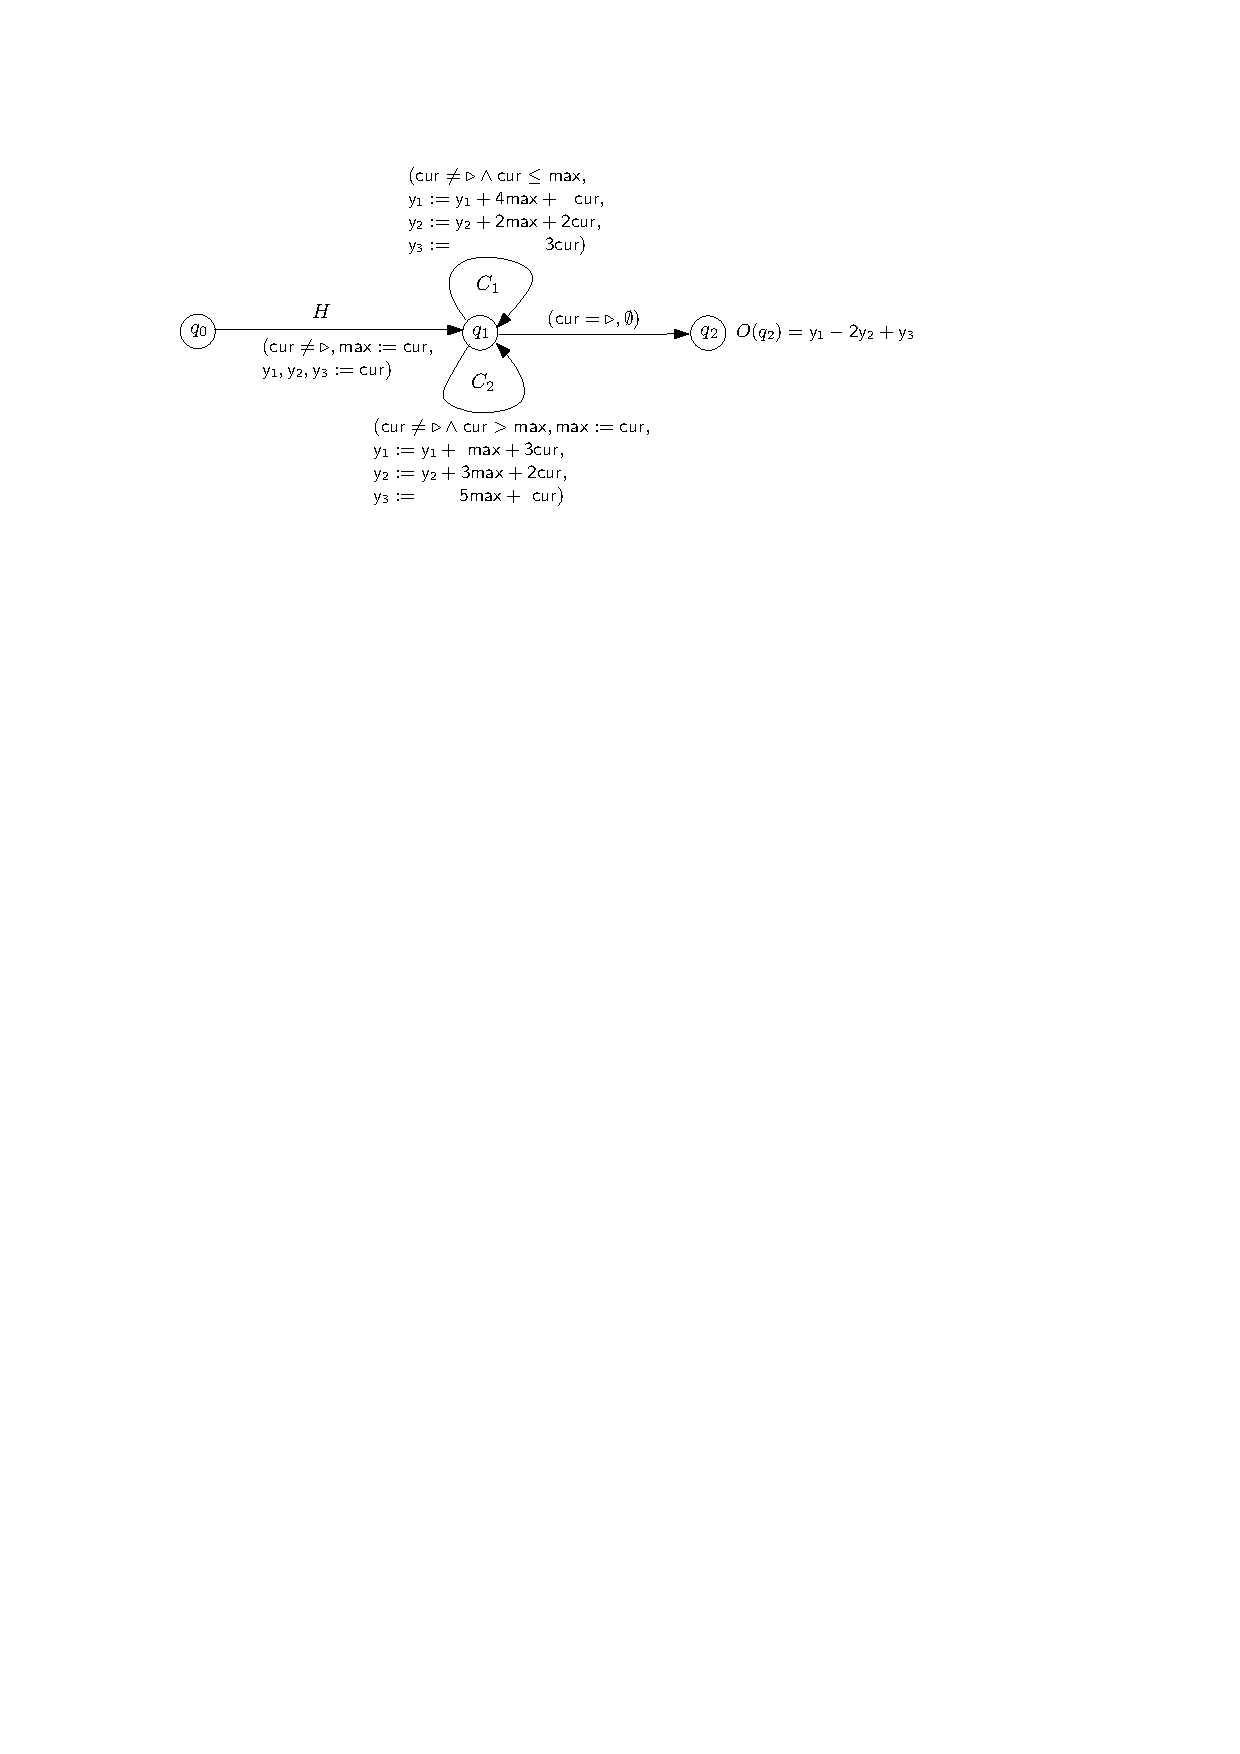
\includegraphics[scale=0.9]{dec-proc-snt-exmp.pdf}
\caption{The SNT $\Ss'_{\max}$: Extending $\Ss_{\max}$ with data variables}\label{fig-dec-proc-snt-exmp}
\end{center}
\end{figure}
%
\end{example}


%!TEX root = main-cav.tex

\vspace{-0.5cm}
\subsection{Decision procedure for generalized lassos}\label{sec-glasso}
\vspace{-1mm}
%
%\yfc{newly added}
In this section, we present a decision procedure for SNTs whose transition graphs are generalized lassos. From Proposition~\ref{prop-sum-cycle}, we know that the coefficients containing the cycle counter variable $\ell$ in $\sumf^{(C^\ell,\initval)}(y_j)$ can be non-zero when $\cstl^{\circled{C}}_{j}=1$. The non-zero coefficients may propagate to the output expression.  In such a case, 
because the SNTs are ``transition-enabled'' (i.e. for any sequence of transitions, a corresponding run exists), %
%if according to the reachability graph, for any $c>0$, there exists a run traversing $C$ more than $c$ times, then 
intuitively, one can pick a run corresponding to a very large $\ell$ so that it dominates the value of the output expression and makes the output non-zero. 
In the decision procedure we are going to present, we first check if the handle of the generalized lasso produces a non-zero output in Step I.
We then check in Step II the coefficients containing $\ell$ in the output expression is non-zero. If this does not happen, then we show in Step III that the non-zero ouput problem of SNT can be reduced to a finite state reachability problem and thus can be easily decided.

Before presenting the decision procedure, we introduce some notations.
Let $e$ be an expression consisting of symbolic values $\initval(z)$ for $z\in X\cup Y$ and variables $\vard_1, \dots, \vard_{s}$ corresponding to the values of the input data word. More specifically, let $e:=\mu_0 + \mu_1 \initval(z_1) +\dots + \mu_{k+l} \initval(z_{k+l}) + \xi_1 \vard_1 + \dots + \xi_{s} \vard_{s}$,
such that $\mu_0,\mu_1,\dots,\mu_{k+l}, \xi_1,\dots,\xi_{s}$ are expressions containing only constants and loop counter variables.
Then we call $\mu_0$ the \emph{constant atom}, $\mu_i \initval(z_i)$ the $\initval(z_i)$-atom for $i\in[k+l]$, and $\xi_j \vard_j$ the $\vard_j$-atom for $j\in[s]$ of the expression $e$. Moreover, $\mu_1, \dots, \mu_{k+l}, \xi_1,\dots, \xi_{s}$ are called the \emph{coefficients} and $\initval(z_1), \dots, \initval(z_{k+l}), \vard_1. \dots, \vard_{s}$ the \emph{subjects} of these atoms.
A non-constant atom is said to be \emph{nontrivial} if its coefficient is \emph{not} identical to zero.

In the rest of this subsection, we assume that the transition graph of $\Ss$ comprises a handle $H=q_0 \xrightarrow{(g_1,\eta_1)} q_1 \dots q_{m-1} \xrightarrow{(g_m,\eta_m)} q_{m}$ and a collection of simple cycles $C_1,\dots,C_n$ such that $q_m$ is the unique state shared by each pair of distinct cycles from $\{C_1,\dots,C_n\}$. Moreover, without loss of generality, we assume that $O(q_m) = a_0 + a_1 x_1 + \dots + a_k x_k + b_1 y_1 + \dots + b_l y_l$, and $O(q)$ is undefined for all the other states $q$.

A \emph{cycle scheme} $\schm$ is a path $C_{i_1}^{\ell_1} C_{i_2}^{\ell_2} \dots C_{i_t}^{\ell_t}$ such that $i_1,\dots,i_t \in [n]$, $\ell_1,\dots, \ell_t \ge 1$, and for each $j\in [t-1]$, $i_j \neq i_{j+1}$. Intuitively, $\schm$ is a path obtained by first iterating $C_{i_1}$ for $\ell_1$ times, then $C_{i_2}$ for $\ell_2$ times, and so on. From Proposition~\ref{prop-sum-cycle} and Corollary~\ref{cor-comp-two-paths}, a symbolic valuation $\sumf^{(\schm,\initval)}$ can be constructed 
to summarize the computation of $\Ss$ on $\schm$. 


\begin{lemma}\label{prop-cycle-schm}
Suppose $\schm=C_{i_1}^{\ell_1} C_{i_2}^{\ell_2} \dots C_{i_t}^{\ell_t}$ is a cycle scheme, and $\initval$ is a symbolic valuation representing the initial values of the control and data variables. 
For all $j' \in  I^{\circled{C_{i_{1}}}}_{pe}$, let $r_{j'}$ be the largest number $r \in [t]$ such that $j'\in\bigcap_{s\in[r]} I^{\circled{C_{i_{s}}}}_{pe}$, i.e., $x_{j'}$ remains persistent when traversing $C_{i_1}^{\ell_1} C_{i_2}^{\ell_2} \dots C_{i_{r_{j'}}}^{\ell_{r_{j'}}}$.
Then for each $j\in [l]$ and $j' \in  I^{\circled{C_{i_{1}}}}_{pe}$, the coefficient of the $\initval(x_{j'})$-atom in $\sumf^{(\schm,\initval)}(y_j)$ is 
\begin{center}
\resizebox{0.8\hsize}{!}{
$e+\sum\limits_{s_1\in[r_{j'}]}  
\left(1+\lambda^{\circled{C_{i_{s_1}}}}_{j} + \dots + (\lambda^{\circled{C_{i_{s_1}}}}_{j})^{\ell_{s_1}-1} \right) \csta^{\circled{C_{i_{s_1}}}}_{j,j'}\prod\limits_{{s_2}\in[{s_1}+1,t]}\left(\lambda^{\circled{C_{i_{s_2}}}}_{j}\right)^{\ell_{s_2}}$},
\end{center}
where (1) $e\!=\!0$ when $r_{j'}\!=\!t$ and (2) $e=(\lambda^{\circled{C_{i_s}}}_{j})^{\ell_s-1} \csta^{\circled{C_{i_{s}}}}_{j,j'} \prod\limits_{{s'}\in[s+1,t]}\left(\lambda^{\circled{C_{i_{s'}}}}_{j}\right)^{\ell_{s'}}$ with $s=r_{j'}+1$ when $r_{j'}<t$.\\
The constant atom of $\sumf^{(\schm,\initval)}(y_j)$ is 
\begin{center}
\resizebox{0.7\hsize}{!}{$
\sum\limits_{{s_1}\in[t]}
\left(1+\lambda^{\circled{C_{i_{s_1}}}}_{j} + \dots + (\lambda^{\circled{C_{i_{s_1}}}}_{j})^{\ell_{s_1}-1} \right)
\cste^{\circled{C_{i_{s_1}}}}_{j} 
\prod\limits_{{s_2}\in[{s_1}+1,t]}\left(\lambda^{\circled{C_{i_{s_2}}}}_{j}\right)^{\ell_{s_2}}$}
\end{center}
Moreover, for all $j\!\in\! [l]$, in $\sumf^{(\schm,\initval)}(y_j)$, only the constant atom and the coefficients of the $\initval(x_{j'})$-atoms with $j' \!\in\!I^{\circled{C_{i_{1}}}}_{pe}$ contain a subexpression of the form $ \mu_\schm \ell_1$ for some~$\mu_\schm\in \intnum$.
\end{lemma}
Notice that above, $\lambda^{\circled{C_{i_{s_1}}}}_j\in\{0,1\}$ for $j\in[l]$ and $s_1\in [t]$. Hence the value of $(1+\lambda^{\circled{C_{i_{s_1}}}}_{j} + \dots + (\lambda^{\circled{C_{i_{s_1}}}}_{j})^{\ell_{s_1}-1} )$ can only be $1$ or $\ell_{s_1}$ and $\left(\lambda^{\circled{C_{i_{s_2}}}}_{j}\right)^{\ell_{s_2}}\in\{0,1\}$.
Therefore, both the constant atom and the coefficient of the $\initval(x_{j'})$-atom with $j'\in I^{\circled{C_{i_{1}}}}_{pe}$ can be rewritten to the form of $c_0+c_1\ell_1+c_2\ell_2+\dots+c_t\ell_t$ for $c_0\ldots c_t\in \intnum$. Note that some of $c_0\ldots c_t$ might be zero.




%We are ready to present the decision procedure. By the ``well-defined'' and ``uniquely-valued'' constraints of normalized SNTs, without loss of generality, we assume that $I^{\circled{H}}_{tr}=[k]$, that is, after traversing $H$, the values of all control variables become defined.
%Under the assumption, 
We are ready to present the decision procedure. At first, we observe that  after traversing $H$ with the initial values of the variables given by $\sval_0$ (recall that $\sval_0$ assigns mutually distinct values to the variables from $X \cup Y$), for each $j' \in I^{\circled{H}}_{tr}$, the value of the control variable $x_{j'}$ becomes $\vard^{\circled{H}}_{\pi^{\circled{H}}(j')}$,  more formally, $\sumf^{(H,\sval_0)}(x_{j'})=\vard^{\circled{H}}_{\pi^{\circled{H}}(j')}$.

In Step I, we check if $\eval{O(q_m)}{\sumf^{(H,\sval_0)}}$ is not identical to zero.
This can be done by checking if the constant-atom or the coefficient of some non-constant atom of the output expression $\eval{O(q_m)}{\sumf^{(H,\sval_0)}}$ is not identical to zero.
%We first find in the reachability graph $G_{\Ss}$ the set of paths $H_{G_{\Ss}}$ corresponding to $H$. Each path in $H_{G_{\Ss}}$ induces an equivalence relation between the subjects of the atoms. 
%For each path $H_{G_{\Ss}}$, we first merge the coefficients of atoms with equivalent subjects. Then we report the output is not identical to zero if the coefficient of some atoms or the constant atom is not zero.
\smallskip\\
\framebox[\textwidth]{
\begin{minipage}{0.95\textwidth}
\noindent {\bf Step I}. Decide whether $\eval{O(q_m)}{\sumf^{(H,\sval_0)}}$ is not identical to zero.
If the answer is yes, then the decision procedure terminates and returns the answer $\ltrue$. Otherwise, go to Step II.
\end{minipage}
}\bigskip

\noindent{\it Complexity analysis of Step I}. Since $\sumf^{(H,\sval_0)}$ can be computed in polynomial time from $H$, it follows that Step I can be done in polynomial time.

\smallskip

The goal of Step II is either showing that in $f=\eval{O(q_m)}{\sumf^{(\schm,\sumf^{(H,\sval_0)})}}$, all subexpressions containing the cycle counter variables are identical to zero and hence can be ignored or showing that $f$ is not identical to zero. Let $\schm=C_{i_1}^{\ell_1} C_{i_2}^{\ell_2} \dots C_{i_t}^{\ell_t}$ be a cycle scheme. From Lemma~\ref{prop-cycle-schm}, for each $j'\in I^{\circled{C_{i_1}}}_{pe}$ and symbolic valuation $\sval$, the only subexpression containing $\ell_1$ in the coefficient of $\initval(x_{j'})$-atom of $\eval{O(q_m)}{\sumf^{(\schm,\initval)}}$ is
\begin{center}
	\resizebox{0.7\hsize}{!}{$
\sum \limits_{1 \le j \le l} 
b_j \left((\cstl^{\circled{C_{i_2}}}_{j})^{\ell_2} \dots (\cstl^{\circled{C_{i_t}}}_{j})^{\ell_t}\right) 
\left(1+\cstl^{\circled{C_{i_1}}}_{j} + \dots + (\cstl^{\circled{C_{i_1}}}_{j})^{\ell_1-1} \right) \csta^{\circled{C_{i_1}}}_{j,j'}.
\hspace{4mm} (\ast)
$}
\end{center}
Since $\cstl^{\circled{C_{i_1}}}_{j}, \cstl^{\circled{C_{i_2}}}_{j}, \dots, \cstl^{\circled{C_{i_t}}}_{j} \in \{0, 1\}$, the expression $(\ast)$  can be rewritten as  
 $\mu_{\schm, (i_1,j')} \ell_1 + \nu_{\schm, (i_1,j')}$ for some integer constants $\mu_{\schm, (i_1,j')}$ and $\nu_{\schm, (i_1,j')}$. 
 
The only subexpression containing $\ell_1$ in the constant atom of  $\eval{O(q_m)}{\sumf^{(\schm,\initval)}}$ is
\begin{center}
	\resizebox{0.7\hsize}{!}{$
\sum \limits_{1 \le j \le l} b_j
\begin{array}{l}
 \left((\lambda^{\circled{C_{i_2}}}_{j})^{\ell_2} \dots (\lambda^{\circled{C_{i_t}}}_{j})^{\ell_t}\right)
\left(1+\lambda^{\circled{C_{i_1}}}_{j} + \dots + (\lambda^{\circled{C_{i_1}}}_{j})^{\ell_1-1} \right) \cste^{\circled{C_{i_1}}}_{j}. \hspace{2mm} (\ast\ast)
\end{array}
$}
\end{center}
%
The expression $(\ast\ast)$ can be rewritten as $\mu_{\schm,(i_1,0)} \ell_1 + \nu_{\schm,(i_1,0)}$ for some integer constants $\mu_{\schm, (i_1,0)}$ and $\nu_{\schm, (i_1,0)}$. If $\mu_{\schm,(i_1,0)}=0$ and $\mu_{\schm,(i_1,j')}=0$ for all $j' \in I^{\circled{C_{i_1}}}_{pe}$, then we can ignore all subexpressions containing the cycle counter variable $\ell_1$ in   $\eval{O(q_m)}{\sumf^{(\schm,\initval)}}$, i.e., the subexpressions $\mu_{\schm,(i_1,0)}\ell_1$ and $\mu_{\schm,(i_1,j')}\ell_1$ for all $j' \in I^{\circled{C_{i_1}}}_{pe}$.\smallskip\\
\framebox[\textwidth]{
	\begin{minipage}{0.95\textwidth}
		\noindent {\bf Step II}. For each $i_1 \in [n]$, check all cycle scheme $\schm=C_{i_1}^{\ell_1} C_{i_2} \dots C_{i_t}$ such that $i_2,\dots,i_t$ are mutually distinct. There are only finitely many this kind of cycle schemes. If 
		one of the following constraints is satisfied, then return $\ltrue$. \\(1) There is $j' \in  I^{\circled{C_{i_1}}}_{pe}$ such that $\mu_{\schm,(i_1,j')} \neq 0$. (2) $\mu_{\schm,(i_1,0)} \neq 0$.
		%
		If the decision procedure has not returned yet, then go to Step III.
	\end{minipage}
}\bigskip

\noindent{\it Complexity analysis of Step II}. Since $i_1,\dots, i_t$ are mutually distinct, the number of cycle schemes $\schm = C_{i_1}^{\ell_1} C_{i_2} \dots C_{i_t}$ in Step II is exponential over the number of cycles in the generalized lasso. Once the cycle scheme is fixed, the two constraints in Step II can be decided in polynomial time. Therefore, the complexity of Step II is exponential over the number of cycles in the generalized lasso.

\smallskip

If there exists $j' \in I^{\circled{C_{i_1}}}_{pe}$ such that $\mu_{\schm,(i_1,j')} \neq 0$, then we let $\vard^{\circled{H}}_{\pi^{\circled{H}}(j')} \neq 0$ and $\ell_1$ be arbitrarily large, so that the coefficient of the  $\vard^{\circled{H}}_{\pi^{\circled{H}}(j')}$-atom in $\eval{O(q_m)}{\sumf^{(\schm,\sumf^{(H,\sval_\bot)})}}$, which includes the expression $\mu_{\schm, (i_1,j')} \ell_1 + \nu_{\schm, (i_1,j')}$, dominates $\eval{O(q_m)}{\sumf^{(\schm,\sumf^{(H,\sval_\bot)})}}$. This is sufficient to make $\eval{O(q_m)}{\sumf^{(\schm,\sumf^{(H,\sval_\bot)})}}$ non-zero. Similarly, if $\mu_{\schm,(i_1,0)} \neq 0$, then we can let $\ell_1$ arbitrarily large to make the expression $\eval{O(q_m)}{\sumf^{(\schm,\sumf^{(H,\sval_\bot)})}}$ non-zero.
Similar arguments can be applied for $\ell_2\dots\ell_n$.

If Step II does not return $\ltrue$, we show below that for all cycle schemes $\schm_1=C_{i_1}^{\ell_1} C_{i_2}^{\ell_2} \dots C_{i_{s_1}}^{\ell_{s_1}}$ with $i_1,i_2,\dots,i_{s_1} \in [n]$, all subexpressions containing cycle counter variables in $\eval{O(q_m)}{\sumf^{(\schm,\initval)}}$ are identical to zero and hence can be removed. Let ${i'_2} \dots {i'_{s_2}}$ be the sequence obtained from $i_2 \dots i_{s,1}$ by keeping just one copy for each duplicated index therein.  
In Step II we already checked a cycle scheme $\schm_2=C_{i_1}^{\ell_1} C_{i'_2} \dots C_{i'_{s_2}}$. Step II guarantees that all subexpressions containing $\ell_1$ in 
$\eval{O(q_m)}{\sumf^{(\schm_2,\initval)}}$ are identical to zero and hence can be removed.
Because for all $j\in[l]$, $\cstl^{^{\circled{C_1}}}_j, \dots, \cstl^{^{\circled{C_n}}}_j \in \{0,1\}$,   $(\lambda^{\circled{C_{i_2}}}_{j})^{\ell_2} \dots (\lambda^{\circled{C_{i_{s_1}}}}_{j})^{\ell_{s_1}} = \lambda^{\circled{C_{i'_2}}}_{j} \dots \lambda^{\circled{C_{i'_{s_2}}}}_{j}$. We proved that the $(\ast)$ and $(\ast\ast)$ style expressions are equivalent in both $\schm_1$ and $\schm_2$.
Hence we can also remove all subexpressions containing $\ell_1$ from  $\eval{O(q_m)}{\sumf^{(\schm_1,\initval)}}$, without affecting its value.
Those subexpressions containing $\ell_2$ can also be removed by considering the cycle scheme $\schm_3=C_{i_2}^{\ell_2} C_{i''_3} \dots C_{i''_{s_3}}$ and applying a similar reasoning, where the sequence ${i''_3} \dots {i''_{s_3}}$ is obtained from ${i_3} \dots  i_{s_1}$, similarly to the construction of ${i'_2} \dots {i'_{s_2}}$ from $i_2 \dots i_{s,1}$. The same applies to all other cycle counter variables $\ell_3,\dots,\ell_{s_1}$.
We use the notation ${\sumf^{(\schm,\initval)}}^-(y_j)$ to denote the expression obtained by removing from the constant atom and coefficients of the non-constant atoms of $\sumf^{(\schm,\initval)}(y_j)$ all subexpressions containing cycle counter variables, for all $y_j \in Y$. 

\begin{lemma}\label{prop-bnd-domain-1}
	Suppose that the decision procedure has not returned $\ltrue$ after Step~II. For each cycle scheme $\schm$, let $f=\eval{O(q_m)}{\sumf^{(\schm, \sumf^{(H,\sval_\bot)})}}$ and $f'=\eval{O(q_m)}{{\sumf^{(\schm, \sumf^{(H,\sval_\bot)})}}^-}$. For all valuation $\rho$, $\eval{f}{\rho}\neq 0$ iff $\eval{f'}{\rho} \neq 0$.
\end{lemma}





\begin{lemma}\label{prop-bnd-domain-2}
Suppose that the decision procedure has not returned yet after Step II. 
For all cycle scheme $\schm$ and $y_j \in Y$, the constant atom and the coefficients of all non-constant atoms in ${\sumf^{(\schm, \sumf^{(H,\initval_\bot)})}}^-(y_j)$ are from a finite set $U \subset \intnum$ comprising \\ (1)
the constant atom and the coefficients of the non-constant atoms in the expression ${\sumf^{(C^{\ell_i}_{i}, \sumf^{(H,\initval_\bot)})}}^-(y_j)$ for $i\in [n]$ and $\ell_i \in \{1,2\}$,\smallskip\\(2) the numbers $\csta^{\circled{C_{s_2}}}_{j,j'} + \cstb^{\circled{C_{s_1}}}_{j,\pi^{\circled{C_{s_1}}}(j')}$ and $\csta^{\circled{C_{s_1}}}_{j, j''} + \csta^{\circled{C_{s_2}}}_{j,j''}$, where  $s_1,s_2 \in [n], j\in[l],j' \in I^{\circled{C_{s_1}}}_{tr} \cap I^{\circled{C_{s_2}}}_{tr},  j'' \in [k]$. 

\end{lemma}

For each cycle scheme $\schm$, an abstraction of ${\sumf^{(\schm, \sumf^{(H,\initval_\bot)})}}^-$, denoted by $\abs(\schm)$,  is the union of the following three sets:
(1)~constant atom: $\{(0, ( {\cste^{(\schm)}_{1}}^-,\dots, {\cste^{(\schm)}_l}^-))\}$. 
(2)~control variable atom: $\{(j', (c_{j',1},\dots, c_{j', l})) \mid j' \in [k]\}$, where $c_{j', j}$ is the coefficient of the ${\sumf^{(\schm,\sumf^{(H,\sval_\bot)})}}^-(x_{j'})$-atom in ${\sumf^{(\schm,\sumf^{(H,\sval_\bot)})}}^-(y_{j})$ for $j\in[l]$. (3)~data variable atom: $\{(k+1, (c_1,\dots,c_l))\}$, where $(c_1,\dots,c_l) \in U^l$ is the coefficients of the $\vard'$-atom in ${(\sumf^{(\schm,\sumf^{(H,\sval_\bot)})}}^-(y_{j})$ for all $j \in [l]$ and $\vard'\not\in \{{\sumf^{(\schm,\sumf^{(H,\sval_\bot)})}}^-(x_{j'})\mid x_{j'}\in X\}$.
Let $\mathscr{A}=\bigcup \{\abs(\schm) \mid \schm \mbox{ a cycle scheme}\}$. Then $\mathscr{A}$ can be constructed as follows. We first compute $\abs(HC_1), \ldots \abs(HC_n)$ and then compute the next abstract elements from them w.r.t. $C_1\ldots C_n$ until reached a fixed point.\medskip\\
\framebox[\textwidth]{
	\begin{minipage}{0.95\textwidth}
		\noindent {\bf Step III} We first construct the set $\mathscr{A}$ and then. 
		\begin{enumerate}
			\item Check whether there is $(0,(c_{0,1},\dots,c_{0,l})) \in \mathscr{A}$ such that $a_0+b_1 c_{0,1}+\dots + b_l c_{0,l} \neq 0$. If the answer is yes, then return $\ltrue$.
			%
			\item Check whether there are $j' \in [k]$ and $(j', (c_{j',1},\dots,c_{j',l})) \in \mathscr{A}$ such that $a_{j'} + b_1 c_{j',1} + \dots + b_l c_{j',l} \neq 0$. If the answer is yes, then return $\ltrue$. 
			%
			\item Check whether there is $(k+1,(c_1,\dots,c_l)) \in \mathscr{A}$ such that $b_1 c_1 + \dots + b_l c_l \neq 0$. If the answer is yes, then return $\ltrue$. 
		\end{enumerate}
		If the decision procedure has not returned yet, return $\lfalse$.
	\end{minipage}
}\smallskip\\

\noindent {\it Complexity analysis of Step III}. The size of the set $U$ is polynomial over the size of the generalized lasso (i.e. the size of the transitions in the generalized lasso). The size of $\mathscr{A}$ is exponential over $l$, the number of data variables. The three conditions in Step III can be checked in time polynomial over the size of $\mathscr{A}$. In summary, the complexity of Step III is exponential over the number of data variables.


\vspace{-2mm}
\subsection{Decision procedure for SNTs}\label{sec-gflat}
\vspace{-1mm}

We generalize the decision procedure for the case that the transition graphs of the SNTs are generalized lassos to the full class of SNTs.
We first define a \emph{generalized multi-lasso} as a sequence $\gmlasso= H_1 (C_{1,1},\dots,C_{1,n_1}) H_2 (C_{2,1},\dots,C_{2,n_2}) \dots H_r (C_{r,1},\dots, C_{r, n_r})$ s.t. (1) for each $s\in[r]$, $H_s=q_{s,1} \xrightarrow{(g_2,\eta_2)} q_{s,2} \dots q_{s,m_s-1} \xrightarrow{(g_{m_s},\eta_{m_s})} q_{s,m_s}$ is a generalized lasso, (2) for $1 \leq s< s' \leq r$, $H_s (C_{s,1},\dots,C_{s, n_s})$ and $H_{s'} (C_{s', 1},\dots,C_{s', n_{s'}})$ are state-disjoint, except the case that when $s'=s+1$, $q_{s, m_s}=q_{s',1}$, and (3) $q_{1,1}=q_0$.

Since the transition graph of $\Ss$ can be seen as a finite collection of generalized multi-lassos, in the following, we shall present the decision procedure by showing how to decide the non-zero output problem for generalized multi-lassos. 

We fix a generalized multi-lasso below and assume without loss of generality that $O(q_{r,m_r})=a_0+a_1 x_1 + \dots + a_k x_k + b_1 y_1  + \dots + b_l y_l$ and $O(q')$ is undefined for every other state $q'$ in $\gmlasso$.

\smallskip
\hspace{8mm} $\gmlasso= H_1 (C_{1,1},\dots,C_{1,n_1}) H_2 (C_{2,1},\dots,C_{2,n_2}) \dots H_r (C_{r,1},\dots, C_{r, n_r})$.

\subsubsection{Step I':} We do the same analysis as in Step I for the path $H_1\dots H_r$.
\hide{\smallskip\\
\framebox[\textwidth]{
	\begin{minipage}{0.95\textwidth}
		\noindent {\bf Step I$'$}. We do the same analysis as in Step I for the path $H_1\dots H_r$.
	\end{minipage}
}\smallskip}
\subsubsection{Step II':}
Let $s\in [1,r-1]$. In order to analyze the set of cycles $\Cc=\{C_{s,1},\dots,C_{s,n_{s}}\}$, next we show how to summarize effect of the path $H_{s+1}\dots H_r$ to $O(q_{s, m_{s}})$, which is shared by all those cycles in $\Cc$.
Suppose that $\eval{O(q_{r,m_r})}{\sumf^{(H_{s+1}\dots H_{r}, \initval)}}=a_0+a_1 \initval(x_1)+ \dots + a_k \initval(x_k) + b_1 \initval(y_1) + \dots + b_l \initval(y_l)+e$, where $e$ is a linear combination of the data variables that represent the data values introduced when traversing $H_{s+1}\dots H_r$. Since we already passed Step I, we know that $e$ should be identical to zero. 
%the constant atom is $a_{s,0}$, the coefficient of the $\initval(x_j)$-atom is $a_{s, j}$ for each $j \in [k]$, and the coefficient of the $\initval(y_{j'})$-atom is $b_{s, j'}$ for each $j' \in [l]$. 
Moreover, we know that $\initval(x_1)\dots\initval(x_k)$ and $\initval(y_1)\ldots \initval(y_l)$ are values of $x_1\dots x_k$ and $y_1 \dots y_l$ at the state $q_{s, m_{s}}$. Therefore, we can summarize the effect of $H_{s+1}\dots H_{r}$ to $q_{s, m_{s}}$ by letting
$O(q_{s, m_{s}}):=a_0+a_1 x_1 + \dots + a_k x_k + b_1 y_1 + \dots + b_l y_l$ and $O(q')$ is undefined for every other state $q'$.\smallskip\\
\framebox[\textwidth]{
	\begin{minipage}{0.95\textwidth}
\noindent {\bf Step II$'$}.  For each $s\in [r]$ and $s'\in [n_s]$, we check each cycle scheme $\schm = C^{\ell_1}_{s,s'} C_{i_{2}} \dots C_{i_{t}}$ such that $C_{i_{2}} \dots C_{i_{t}}\in \{C_{s, 1}, \dots, C_{s,n_s},\dots, C_{r,1}, \dots, C_{r,n_r}\}$ and $C_{i_{2}} \dots C_{i_{t}}$ are mutually distinct by performing an analysis of the expression $\eval{ O(q_{s, m_{s}})} {\sumf^{(\schm,\sumf^{(H_1 \dots H_{s}, \initval)} ) } }$, in a way similar to Step II. If the decision procedure does not return during the analysis, then go to Step III$'$.
	\end{minipage}
}\bigskip\\
Intuitively, in Step II$'$, during the analysis of $\eval{ O(q_{s, m_{s}})} {\sumf^{(\schm,\sumf^{(H_1 \dots H_{s}, \initval)} ) } }$, the effect of the paths $H_{s+1},  \dots,  H_r$ and the cycles $C_{i_{2}}, \dots, C_{i_{t}}$ to the atom coefficients containing cycle counter variables are expressions of the form $\cstl^{\circled{H_{s+1}}}_j \dots \cstl^{\circled{H_{r}}}_j  \cstl^{\circled{C_{i_{2}}}}_j \dots \cstl^{\circled{C_{i_{t}}}}_j $ for $j \in [l]$. Since $O(q_{s, m_{s}})$ has already taken into consideration the expressions $\cstl^{\circled{H_{s+1}}}_j \dots \cstl^{\circled{H_{r}}}_j$ for $j \in [l]$. In Step II$'$, we can do the analysis as if we have a generalized lasso where the handle is $H_1\dots H_s$ and the collection of cycles is $\{C_{s,1},\dots, C_{s,n_s}$, $\dots$, $C_{r,1},\dots, C_{r,n_r}\}$. 
%$\schm=C^{\ell_{s, 1}}_{i_{s,1}} \dots C^{\ell_{s, t_s}}_{i_{s, t_s}} C^{\ell_{s+1, 1}}_{i_{s+1, 1} } \dots C^{\ell_{s+1, t_{s+1}}}_{i_{s+1, t_{s+1}} } \dots C^{\ell_{r, 1}}_{i_{r,1}} \dots C^{\ell_{r, t_r}}_{i_{r, t_r}} $, where for each $s': s \le s' \le r$, $i_{s',1},\dots, i_{s', t_{s'}} \in [n_{s'}]$, 
%%%%%%%%%%%%%%%%%%%%%%%%%%%%%%%%%%%%%%%%%%%%%%%%%%%
%%%%%%%%%%%%%%%%%%%%%%%%%%%%%%%%%%%%%%%%%%%%%%%%%%%
%%%%%%%%%%%%%%%%%%%%%%%%%%%%%%%%%%%%%%%%%%%%%%%%%%%
\hide
{
At first, by using $O(q_m)$, we do the following computation, similarly to Step II: For each $i_1: 1 \le i_1 \le n$, if there are a cycle scheme $\schm$  
$HC_{i_1}^{\ell_1} C_{i_2}^{\ell_2} \dots C_{i_t}^{\ell_t}
$
or 
$HC_{i_1}^{\ell_1} C_{i_2}^{\ell_2} \dots C_{i_t}^{\ell_t} (C'_{i'_1})^{\ell'_1} (C'_{i'_2})^{\ell'_2} \dots (C'_{i'_{t'}})^{\ell'_{t'}}$,
and $j' \le k$ such that 
\begin{itemize}
\item $i_2,\dots,i_t \le n$ are mutually distinct, $\ell_2 = \dots = \ell_t = 1$, 
%
\item $i'_1,\dots,i'_{t'} \le n'$ are mutually distinct, $\ell'_2 = \dots = \ell'_{t'} = 1$, 
%
\item $\pi_{C_{i_1}}(j')=j'$, and $\mu_{\schm,(i_1,j')} \neq 0$ (recall that $\mu_{\schm,(i_1,j')}$ is obtained from the coefficient of $d^{(0)}_{\pi_H(j')-k}$ in  $\chi_\schm(O(q_m))$), 
\end{itemize}
then return $\ltrue$. 

Then by using $O(q'_{m'})$, we do the following: For each $i'_1: 1 \le i'_1 \le n'$, if there are a cycle scheme $\schm' =(C'_{i'_1})^{\ell'_1} (C'_{i'_2})^{\ell'_2} \dots (C'_{i'_{t'}})^{\ell'_{t'}}$, and $j' \le k$ such that
\begin{itemize}
\item $i'_2,\dots,i'_t \le n'$ are mutually distinct, $\ell'_2 = \dots = \ell'_t = 1$, 
%
\item $\pi_{C'_{i_1}}(j')=j'$, and $\mu_{\schm',(i'_1,j')} \neq 0$ (here $\mu_{\schm',(i_1,j')}$ is obtained from the coefficient of $d''_{j'}$ in  $\chi_{\schm'}(O(q'_{m'}))$, where $d''_1,\dots,d''_k$ denote the initial data values of $x_1,\dots,x_k$ respectively),
\end{itemize}
then return $\ltrue$. 

Similarly, we can apply an analysis for the constant coefficient to $\chi_\schm(O(q_m))$. 


If the decision procedure has not return yet, then go to Step III$'$. \qed
}
%%%%%%%%%%%%%%%%%%%%%%%%%%%%%%%%%%%%%%%%%%%%%%%%%%%
%%%%%%%%%%%%%%%%%%%%%%%%%%%%%%%%%%%%%%%%%%%%%%%%%%%
%%%%%%%%%%%%%%%%%%%%%%%%%%%%%%%%%%%%%%%%%%%%%%%%%%%
\subsubsection{Step III':}
After Step II$'$, if the decision procedure has not returned yet, then similar to Lemma~\ref{prop-bnd-domain-2}, the following hold.
\begin{itemize}
\item For each $s \in [r]$ and each path $\schm=H_1 \schm_1 H_2 \dots H_s \schm_s$ such that for each $s'\in [s]$, $\schm_{s'}$ is a cycle scheme over the collection of cycles $\{C_{s',1},\dots,C_{s',n_{s'}}\}$, it holds that the constant atom and all the coefficients of the non-constant atoms in ${\sumf^{(\schm,\sval_\bot)}}^-(y_j)$ are from a bounded domain $U$.
%
\item Moreover,  an abstraction of $\schm$, denoted by $\abs(\schm)$, can be defined, so that $\mathscr{A}$, which contains the set of $\abs(\schm)$ for the paths $\schm=H_1 \schm_1 H_2 \dots H_s \schm_s$ (where $s \in [r]$), can be computed effectively from 
$H_1, C_{1,1}, \dots, C_{1,n_1},H_2,\dots, H_r,C_{r,1},\dots, C_{r,n_r}$.
\end{itemize}
%Similarly to the generalized lassos, we can construct a finite state automaton $\Aa'$ from $\chi_H,\chi_{C_1},\dots,\chi_{C_n},\chi_{H'}, \chi_{C'_1},\dots,\chi_{C'_{n'}}$ to record the coefficients in the states and simulate the evolvement of these coefficients. The final states of $\Aa$ represent the coefficients obtained when reaching the state $q'_{m'}$ in $\Ss$. 
\framebox[\textwidth]{
	\begin{minipage}{0.95\textwidth}
\noindent {\bf Step III$'$}. We apply the same analysis to $\mathscr{A}$ as in Step III. If the procedure does not return during the analysis, return $\lfalse$.
	\end{minipage}
}\bigskip

\noindent {\it Complexity analysis of Step I$'$-III$'$}. The complexity of Step I$'$ is polynomial over the the maximum length of generalized multi-lassos in $\Ss$. The complexity of Step II$''$ is exponential over the maximum number of simple cycles in generalized multi-lassos. The complexity of Step III$'$ is still exponential over the number of data variables in $\Ss$.



%!TEX root = main-cav.tex


\section{Extensions}
\label{sec:cases}

\begin{figure}
	\centering
	\lstset{language=C,
		basicstyle=\ttfamily\scriptsize}
	\begin{tabular}{|c|c|c|}
		\hline
		\begin{minipage}[t]{0.2\textwidth}
		\vspace{-0.5cm}
			\begin{lstlisting}[mathescape=true]
int avg() {
 sum:=$\cur$;
 cnt:=0;$\nnext$;
 loop{
  sum+=$\cur$;
  cnt+=1;
  $\nnext$;};
 ret sum/cnt;}
			\end{lstlisting}
		\end{minipage}&
		\begin{minipage}[t]{0.4\textwidth}
		\vspace{-0.5cm}
\begin{lstlisting}[mathescape=true]
int MAD() {
 sum:=$\cur$;cnt:=0;$\nnext$;
 loop{sum+=$\cur$;cnt+=1;$\nnext$;};
 avg:= sum/cnt;mad:=0;$\init$;
 loop{
  if($\cur$<avg){mad=mad+(avg-$\cur$);}
  else{mad=mad+($\cur$-avg);};$\nnext$;};
 ret mad/cnt;}
\end{lstlisting}
		\end{minipage}&
		\begin{minipage}[t]{0.4\textwidth}
		\vspace{-0.5cm}
			\begin{lstlisting}[mathescape=true]
int SD() {
 sum:=$\cur$;cnt:=0;$\nnext$;
 loop{sum+=$\cur$;cnt+=1;$\nnext$;};
 avg:= sum/cnt;sd:=0;$\init$;
 loop{
  sd+=($\cur$-avg)*($\cur$-avg);$\nnext$;
 };
 ret SQRT(sd/cnt);}
			\end{lstlisting}
		\end{minipage}\\
		\hline		
	\end{tabular}
	\caption{More Challenging Examples of Reducers Performing Data Analytics Operations}
	\label{fig:examples2}
\end{figure}
%\vspace{-0.5cm}

In this section, we discuss more challenging extensions. 
For cases with multiplication, division, or other more complicated functions at the return point, e.g., the \texttt{avg} case, we can model them as an \emph{uninterpreted $k$-ary function} and verify that all $k$ parameters of the uninterpreted functions remain the same no matter how the input is permuted, e.g., the \texttt{avg} program always produces the same \texttt{sum} and \texttt{cnt} for all permutation of the same input data word. This is a \emph{sound} but \emph{incomplete} procedure for verifying programs of this type. Nevertheless, it is not often that a  practical program for data analytics produces, e.g., $2q/2r$ from some input and $q/r$ for its permutation. Hence this procedure is often enough for proving commutativity for real world programs.

The case \texttt{MAD} (Mean Absolute Deviation) is a bit more involved. Beside the division operator $/$ that also occurs in the \texttt{avg} example, it uses a new iterator operation $\init$, which resets $\cur$ to the head of the input data word. The strategy to verify this program is to divide the task into two parts: (1) ensure that the value of \texttt{avg} is independent of the order of the input, (2) treat \texttt{avg} as a control variable whose value is never updated and then check if the 2nd half of the program (c.f., Fig.~\ref{fig:examples3}) is commutative. 

\begin{wrapfigure}{r}{0.4\textwidth}
	\vspace{-0.8cm}
	\lstset{language=C,
		basicstyle=\ttfamily\scriptsize}
	\begin{lstlisting}[mathescape=true]
int MAD2() {
 avg:= $\cur$;$\nnext$;
 loop{
  if($\cur$<avg){mad+=avg-$\cur$;}
  else{mad+=$\cur$-avg;}
  $\nnext$;}
 ret mad/cnt;}
	\end{lstlisting}	
	\vspace{-0.4cm}
	\caption{The 2nd half of MAD}
	\label{fig:examples3}
	\vspace{-0.7cm}
\end{wrapfigure}
We handle the division at the end of the program in Fig.~\ref{fig:examples3} in the same way as we did for the \texttt{avg} program. The guarantee we obtain after the corresponding SNT is checked to be commutative is that the program outputs the same value for any value of \texttt{avg} and any permutation of  the input data word. 


%The latter requires an extension to the SNT decision problems. Given a data word $w$, we say a data word $w'$ is a $k$-permutation of $w$ iff there exists $\sigma_k\in S_{|w|}$ such that $\sigma_k(i)=i$ for $i \in [k]$ and $w'=\sigma_k(w)$. In words, $\sigma_k$ is a permutation of length $|w|$ such that it does not change the first $k$ elements. 


% A \emph{$k$-commutativity problem} of a SNT $\Ss$ asks whether for each data word $w$ and its $k$-permutation $w'$, $\Ss(w)=\Ss(w')$. The problem can be reduced to SNT equivalence problems in a similar way to the standard commutativity problem.

%\begin{proposition}\label{prop-snt-kcmm-to-eqv}
%	The $k$-commutativity problem of SNTs is reduced to the equivalence problem of SNTs in exponential time. 
%\end{proposition}




The case \texttt{SD} (Standard Deviation) is more challenging. The main difficulty comes from the use of multiplication in the middle of the program (instead of at the return point). In order to have a sound procedure to verify this kind of programs, we can extend the transitions of SNTs to include uninterpreted $k$-ary functions. However, this is not a trivial extension and we consider it as future work.




%!TEX root = main-cav.tex
	
\section{Conclusion}
\label{sec:conclusion}

%From the analysis of the commutativity of reducers in \cite{XZZ+14}, the commutativity of a reducer in a sequential composition of map-reduce jobs may depend on some implicit data properties guaranteed by the preceding map-reduce jobs. Therefore, to analyze the commutativity of a reducer in a sequential composition of map-reduce jobs, we may need model both mappers and reducers and do a backward analysis.

The contribution of the paper is twofold. We propose a verifiable programming language for reducers. Although it is still far away from a practical programming language, we believe that some ideas behind our language (e.g., the separation of control variables and data variables) would be valuable for the design of a practical reducer language. On the other hand, we propose the model of streaming numerical transducers, a transducer model over infinite alphabets. To our best knowledge, this is the first decidable automata model over infinite alphabets that allows linear arithmetics over the input values and the integer variables. Although we required that the transition graphs of SNTs are generalized flat,  SNTs with such kind of transition graphs turn out to be quite powerful, since they are capable of simulating reducer programs without nested loops, which is a typical scenario of reducer programs in practice.


\subsubsection{Acknowledgements.} Yu-Fang Chen is partially supported by the MOST project No. 103-2221-E-001-019-MY3. Zhilin Wu is partially supported by the NSFC grants No.\ 61100062, 61272135, 61472474, and 61572478.

% , parameterized counter automata, integer VASS

%restate the contribution of our work. (1) hint for verifiable reducer/list manipulating program language (2) SNT is a first autoamta with infinite alphabet supporting presburgh arithemetic over input and variables.


\bibliographystyle{abbrv}
\bibliography{data}

\newpage

%!TEX root = main-cav.tex

\begin{appendix}

\section{Formal Semantics of the Programming Language}
\begin{figure}
	\hspace{-0.4cm}
	\scalebox{0.9}{
		\begin{tabular}{|l|l|}
			\hline
			Transitions&
			Side Condition\\
			\hline
			$(y := e;p, w, \rho) \longrightarrow (p, w, \rho')$&
			$\rho'=\rho[\eval{e}{\rho}/y]$\\
			
%			$\rho'(z) =\rho(z)$ for $z\neq y$, $\rho'(y) = \eval{\rho}{e}$\\
			
			$(y \addeq e;p, w, \rho) \longrightarrow (p, w, \rho')$&
			$\rho'=\rho[\eval{y+e}{\rho}/y]$\\
%			$\rho'(z) =\rho(z)$ for $z\neq y$, $\rho'(y) = \eval{y+e}{\rho}$\\
			
			$(\ite{g}{s_1}{s_2};p, w, \rho) \longrightarrow (s_1;p, w, \rho)$&
			$\rho \models g$\\
			
			$(\ite{g}{s_1}{s_2};p, w, \rho) \longrightarrow (s_2;p, w, \rho)$& $\rho \not \models g$\\
			
			$(\nnext;p, w, \rho) \longrightarrow (p, \tail(w), \rho')$&
			$\rho'=\rho[\head(\tail(w))/\cur]$ if $w\neq \epsilon$ \\

			$(\nnext;p, w, \rho) \longrightarrow (p, \epsilon, \rho_\bot)$&
			 if $w = \epsilon$\\

			
			$(x':=x;p, w, \rho) \longrightarrow (p, w, \rho')$&
			$\rho'  =\rho[\rho(x)/x']$\\
			
			$(\loopL{s};\mbox{ret }r, w, \rho) \longrightarrow (s;\loopL{s};\mbox{ret }r, w, \rho)$& \\
			
			$(\loopL{s};\mbox{ret }r, \epsilon, \rho) \longrightarrow (\mbox{ret }r,  \epsilon, \rho)$& 	\\	
			\hline
			
		\end{tabular}
	}
	\caption{The Semantics of the Programming Language}
	\label{fig:semantics}
\end{figure}


Formally, the semantics of a program $p$ in the programming language is defined as a transition system in Fig.~\ref{fig:semantics}. Let $p$ be a reducer program and $w$ be an input data word.  Each configuration of the transition system is a triple $(p', w', \rho)$, where $p'$ is a program, $w'$ is a suffix of $w$, and $\rho$ is an valuation over $X^+\cup Y$ such that $\rho(\cur)=\head(w')$. 
Let $\rho_w$ be an assignment such that $\rho_w(\cur)=\head(w)$ and $\rho_w(z)=\bot$ for $z \in X \cup Y$.
The initial configuration is $(p, w, \rho_w)$.
We use $p(w)$ to denote the \emph{output} of $p$ on $w$. Then $p(w) =d$ if there exists a path from the initial configuration $(p, w, \rho_w)$ to some return configuration $(\mbox{ret }r,  \epsilon, \rho_r)$ such that $
\eval{r}{\rho_r}=d$. Otherwise, $p(w)=\bot$. Since the program is deterministic, i.e., each input data word has at most one output, the semantics of $p$ is well-defined.

\section{Proofs in Section~\ref{sec:def-snt}}




\newcommand\assume{\mathsf{assume}}

\newcommand\loc{\mathfrak{l}}

\noindent {\bf Proposition~\ref{prop-mrprog-to-snt}}.
{\it 
For each reducer program $p$, an equivalent SNT $\Ss$ can be constructed.
}

\smallskip

\begin{proof}
We introduce a few notations first.

Let $s$ be a loop-free program. An \emph{execution path} $\pi$ of $s$ is a maximal path in the control flow graph of $s$ (here we use the standard definition of control flow graphs). Each execution path $\pi$ corresponds to a program $s_\pi$ obtained by sequentially composing the statements in $\pi$, where the statements $\assume(g)$ are used to represent the guards $g$. Then $s$ can be seen as a union of $s_\pi$, where $\pi$ ranges over the execution paths of $s$. 

Let $p$ be a reducer program of the form $s_1; \nnext; \loopL{s_2;\nnext}$; ret $r$.  In the following, we show how to construct an SNT $\Ss_p$ to simulate $p$.

The loop body $s_2;\nnext$ can be seen as a union of programs $p_\pi$ for execution paths $\pi$. We assume that no two distinct programs $p_\pi$ share locations. We first transform the loop into a collection of state-disjoint cycles $C_\pi$, one for each program $p_\pi$.  Let us focus on a program $p_\pi$. The set of states in $P_\pi$ comprises the location $\loc_0$ which is the entry point of the loop, and the locations succeeding each $\nnext$ statement in $p_\pi$. Moreover, we identify the location succeeding the last $\nnext$ statement and the entry point. The effect of the subprogram $s'$ between two successive $\nnext$ statements in the locations $\loc_1,\loc_2$ can be summarized into a transition $(\loc_0, g', \eta', \loc_1)$ resp. $(\loc_1, g', \eta', \loc_2)$ of $p_\pi$. This is possible due to the following two constraints: 1) the conditions $g$ in the statements $\ite{g}{s'_1}{s'_2}$  of $p_\pi$ are the conjunctions of $\cur \odot c$ and $\cur \odot x$, 2) the assignments to the control variables are of the form $x:=x'$ for $x' \in X^+$, and the assignments to the data variables are of the form $y:=e$ and $y {+=} e$, where $e$ contains only control variables or $\cur$. As a result of the two constraints, we can trace the evolvement of the values of the control variables and simulate all the statements $\assume(g)$ occurring in $s'$ by a guard $g'$ (obtained from these guards $g$ by some variable substitutions),  moreover, the effects of all the assignments therein can be summarized into an assignment function $\eta'$.  Similarly, we can do the same for the subprogram between the entry point and the first $\nnext$ statement of $p_\pi$.

In addition, each execution path of $s_1;\nnext$ can be simulated by a simple path of transitions of $\Ss_p$, which ends in the state $\loc_0$, the entry point of the loop.

The output function $O_p$ of $\Ss_p$ is defined as follow: $O_p(\loc_0) = r$ and $O(\loc)$ is undefined for each other state $\loc$.\qed
\end{proof}

\hide{
\begin{algorithm}[H]
	%  \SetAlgoLine
	\KwData{A reducer program $p$}
	$Q=\{q_0\}, \delta=\emptyset, O=\emptyset$, $\mathsf{toState}(p) =q_0$, $\mathsf{toVisit}=\{(\mathsf{toState}(p),p,\ltrue,\emptyset)\}$\;
	\While{$\mathsf{toVisit}\neq \emptyset$}{
		remove $(q,p,g,\eta)$ from $\mathsf{toVisit}$\;
		\Switch{$p$}{
			\lCase{$y := e;p'$,$y \addeq e;p'$,$x'=x;p'$: }{add $(q,p',g,\eta[e/y])$, $(q,p',g,\eta[(y+e)/y])$, $(q,p',g,\eta[x'/x])$ to $\mathsf{toVisit}$, respectively}
			\lCase{$\ite{g'}{s_1}{s_2};p'$: }{add both $(q,s_1;p',g\wedge g',\eta)$ and $(q,s_2;p',g\wedge \neg g',\eta)$ to $\mathsf{toVisit}$}
			\lCase{$\loopL{s;}\mbox{ret }r$: }{add both $(q,s;\loopL{s;}\mbox{ret }r,g,\eta)$ and $(q,\mbox{ret }r, g,\eta)$ to $\mathsf{toVisit}$}
			\lCase{$\nnext;p'$: }{\label{alg:next}
				\uIf{$\mathsf{toState}(p') \not\in Q$}{add $(\mathsf{toState}(p'),p',\ltrue,\emptyset)$ to $\mathsf{toVisit}$ and add $\mathsf{toState}(p')$ to $Q$}
				add $(q, \mathsf{toState}(p'),g,\eta)$ to $\delta$
			}
			\lCase{$\mbox{ret }r: $}{\label{alg:output}
				add a fresh state $q_r$ to $Q$, 
				add $(q, q_r,g,\eta)$ to $\delta$, and $O:=O[r/q_r]$}
		}
	}
	\Return $(Q,X,Y,\delta, \mathsf{toState}(p),O)$\;
	
	\caption{Translate a Reducer Program to a SNT}
	\label{fig:reducer2SNT}
\end{algorithm}
We use a tuple $(q,p,g,\eta)$ to store intermediate results of the translation, where $q$ is the source SNT state, $p$ is a reducer program, $g$ is a guard, and $\eta$ is an assignment.
The algorithm begins with the tuple $(p,p,\ltrue,\emptyset)$. The algorithm add a transition to SNT only when a $\nnext$ statement is encountered (line~\ref{alg:next}). When a $\mbox{ret }r$ statement is encountered, the algorithm adds a fresh state $q_r$ to the SNT and extends the output function to $O[r/q_r]$ (line~\ref{alg:output}).

The SNT returned from Algorithm~\ref{fig:reducer2SNT} is not yet generalized flat. It might have cycles sharing more than one states. All the cycles coming from the loop and branches inside the loop. There must be at least one state $s$ shared by all cycles. Therefore, we can make it generalized flat by duplicating all shared stated other than $s$ so all cycles will have their own copy of the shared states other than $s$.  
}

\vspace{4mm}

\noindent {\bf Proposition~\ref{prop-snt-cmm-to-eqv}}. 
\emph{The commutativity problem of SNTs is reduced to the equivalence problem of SNTs in exponential time}.

\begin{proof}
Suppose that $\Ss=(Q, X, Y, \delta, q_0, O)$ is an SNT such that $X=\{x_1,\dots,x_k\}$ and $Y=\{y_1,\dots,y_l\}$. Without loss of generality, we assume that the output of $\Ss$ is defined only for data words of length at least two. We will construct two SNTs $\Ss_1$ and $\Ss_2$ so that $\Ss$ is commutative iff $\Ss$ is equivalent to both $\Ss_1$ and $\Ss_2$.
\begin{itemize}
\item The intuition of $\Ss_1$ is that over a data word $w=d_1 d_2 d_3 \dots d_n$ with $n\ge 2$, $\Ss_1$ simulates the run of $\Ss$ over $d_2 d_1 d_3 \dots d_n$, that is, the data word obtained from $w$ by swapping the first two data values.
%
\item The intuition of $\Ss_2$ is that over a data word $w=d_1 d_2 d_3 \dots d_n$ with $n\ge 2$, $\Ss_1$ simulates the run of $\Ss$ over $d_2 d_3 \dots d_n d_1$, that is, the data word obtained from $w$ by moving the first data value to the end. 
\end{itemize}
The correctness of this reduction follows from Proposition 1 in \cite{CHSW15}.

\smallskip

\noindent {\it The construction of $\Ss_1$}.

Intuitively, over a data word $w=d_1d_2 d_3 \dots d_n$, we introduce an additional control variable $x'$ to store $d_1$, then simulates the run of $\Ss$ over $d_2 d_1 d_3 \dots d_n$ as follows: When reading $d_2$ in $w$, the data variables are updated properly by letting $x'$ to represent $d_1$ and $\cur$ to represent $d_2$.

Without loss of generality, we assume that for each pair of transitions $q_0 \xrightarrow{(g_1,\eta_1)} q_1 \xrightarrow{(g_2,\eta_2)} q_2$ starting from the initial state $q_0$ in $\Ss$, the following constraints are satisfied,
\begin{itemize}
\item $g_1$ does not contain any variable from $X$ (otherwise, $g_1$ would be evaluated to $\lfalse$),
%
\item for each variable $x \in X$ such that $x$ occurs in $g_2$, it holds that $x \in \dom(\eta_1)$,
%
\item after these two transitions, the values of all the variables from $\dom(\eta_1) \cup \dom(\eta_2)$ are defined, more specifically, for each $y \in Y \cap \dom(\eta_2)$ and each $z \in \vars(\eta_2(y))$, it holds that $z \in \dom(\eta_1)$.
\end{itemize}

Let $q'_{0},q'_{1} \not \in Q$ and $x' \not \in X$. Then $\Ss_1 = (Q \cup \{q'_{0},q'_1\}, X \cup \{x'\}, Y, \delta_1, q'_{0}, O_1)$ such that 
\begin{itemize}
\item $O_1(q'_0)$ and $O_1(q'_1)$ are undefined, and for each $q \in Q$, $O_1(q)=O(q)$,
%
\item $\delta_1$ is constructed from $\delta$ as follows,
\begin{itemize}
\item each element of $\delta$ is an element of $\delta_1$,
%
\item for each pair of transitions $q_0 \xrightarrow{(g_1,\eta_1)} q_1 \xrightarrow{(g_2,\eta_2)} q_2$ in $\Ss$, we add the transitions $(q_0, \ltrue, \eta'_1, q'_1)$ and $(q'_1, g', \eta'_2, q_2)$ into $\delta_1$, where $\eta'_1,g',\eta'_2$ are defined in the following. Suppose for each $y_j \in Y \cap \dom(\eta_1)$, $\eta_1(y_j)=a_{j} + b_{j}\cur$, and for each $y_j \in Y \cap \dom(\eta_2)$, 
\[\eta_2(y_j)= y_j + a'_{j} + b'_{j,0}  \cur + \sum\limits_{x_{j'} \in \dom(\eta_1)} b'_{j,j'} x_{j'},\] 
or 
\[
\eta_2(y_j) = a'_{j} + b'_{j,0} \cur + \sum \limits_{x_{j'} \in \dom(\eta_1)} b'_{j,j'} x_{j'} .
\]
Then $\eta'_1, g', \eta'_2$ are defined as follows.
\begin{itemize}
\item $\eta'_1(x')=\cur$, for each $x \in X \cap \dom(\eta_2)$, $\eta'_1(x)=\cur$, and for all the other variables $z$ from $X \cup Y$, $\eta'_1(z)$ is undefined.
%
\item $g' = g_1 \wedge g'_2$, where $g'_2$ is obtained from $g_2$ by replacing $\cur$ with $x'$, and each $x \in X$ with $\cur$.
%
\item For each $x \in X$, if $x \in \dom(\eta_2)$, then $\eta'_2(x)$ is undefined, otherwise, if $x \in \dom(\eta_1)$, then $\eta'_2(x)=\cur$, otherwise, $\eta'_2(x)$ is undefined.
%
\item For each $y_j \in Y$, if $y_j \in \dom(\eta_2)$, then 
\[
\begin{array}{l c l}
\eta'_2(y_j) & = & (a_{j} + b_{j}\cur) + a'_{j} + b'_{j,0} x' + \sum \limits_{x_{j'} \in \dom(\eta_1)} b'_{j,j'} \cur \\
& = & (a_{j} + a'_{j}) + b'_{j,0} x' + (b_{j}  + \sum \limits_{x_{j'} \in \dom(\eta_1)} b'_{j,j'} )\cur,
\end{array}
\]
or 
\[
\begin{array}{l c l}
\eta'_2(y_j) & = & a'_{j} + b'_{j,0} x' + \sum \limits_{x_{j'} \in \dom(\eta_1)} b'_{j,j'} \cur  \\
& = & a'_{j} + b_{j,0} x' + (\sum \limits_{x_{j'} \in \dom(\eta_1)} b'_{j,j'}  )\cur.
\end{array}
\]
%
Otherwise, if $y_j \in \dom(\eta_1)$, then $\eta'_2(y_j)= a_{j} + b_{j} \cur$. Otherwise, $\eta'_2(y_j)$ is undefined.
\end{itemize}
\end{itemize}
\end{itemize}
It is easy to see that the size of $\Ss_1$ is polynomial with respect to the size of $\Ss$.

\smallskip

\noindent {\it The construction of $\Ss_2$}.

Intuitively, over a data word $w=d_1\dots d_n$, we introduce an additional control variable $x'$ to store $d_1$, then simulates the run of $\Ss$ over $d_2\dots d_n d_1$: When reaching the end of $w$, $\Ss_2$ outputs immediately by using $x'$ to represent $d_1$ and simulating the last transition of $\Ss$ over $d_2 \dots d_n d_1$. In order to simulate \emph{deterministically} the last transition of $\Ss$ over $d_2 \dots d_n d_1$ when reading the end of $w$ (since SNTs are required to be deterministic), we need record in the states of $\Ss_2$ the relationship between $d_1$ and all the values stored in the control variables. This implies an exponential blow-up of the size of $\Ss_2$ with respect to $\Ss$.

Let $c_{max}$ and $c_{min}$ denote the maximum resp. minimum constant occurring the guards of the transitions of $\Ss$. As a convention, let $c_{max}=c_{min}=0$ if no constants occur in $\Ss$.

Suppose $q'_{0} \not \in Q$ and $x' \not \in X$. Then $\Ss_2 = (Q', Y, \delta_2, q'_{0}, O_2)$, where $O',\delta_2,O_2$ are defined as follows. 
\begin{itemize}
\item $Q' = \{q'_0\} \cup \left(Q \times \left([c_{\min}, c_{\max}] \cup \{-\infty,+\infty\}\right) \times X^{\{=, <, >,\bot\}} \right)$, where in a state $(q,(c, o)) \in Q'$, the third component $o$ denotes the relationship between $x'$ and $x$, e.g. $o(x)=<$ means that $x' < x$.
%
\item $\delta_2$ is defined as follows, 
\begin{itemize}
\item for each $c \in [c_{min}, c_{max}] \cup \{-\infty,+\infty\}$, $\delta_2$ contains $(q'_0,\ltrue,\eta, (q_0,(c, o_0)))$, where $\dom(\eta)=\{x'\}$, $\eta(x')=\cur$, and $o_0(x) = \bot$ for each $x \in X$,
%
\item for each $(q,g,\eta,q') \in \delta$ and $(q,(c,o)) \in Q'$ such that $g \wedge \bigwedge \limits_{x \in X, o(x) \neq \bot} x'\ o(x)\ x$ is satisfiable, $\delta_2$ contains the following three transitions, 
$(q,(c,o)) \xrightarrow{(g \wedge \cur = x', \eta)} (q',(c,o'_1))$, 
$(q,(c,o)) \xrightarrow{(g \wedge \cur< x', \eta)}  (q',(c,o'_2))$,
and  $(q,(c,o)) \xrightarrow{(g \wedge \cur > x', \eta)} (q',(c,o'_3))$, where 
for each $x \in X$, if $x \in \dom(\eta)$, then $o'_1(x) := \ =$, $o'_2(x):=\ >$, and $o'_3(x) :=\ <$, otherwise, $o'_1(x) = o'_2(x) = o'_3(x) := o(x)$.
\end{itemize}
%
\item $O_2$ is defined as follows: Let $(q,(c,o)) \in Q'$  such that there is $(q,g,\eta,q') \in \delta$ satisfying that $\left(g_c \wedge \bigwedge \limits_{x \in X, o(x) \neq \bot} \cur\ o(x)\ x \right) \models g$, and $O(q')$ is defined, where $g_c := \cur = c$ if $c \in [c_{min}, c_{max}]$, $g_c:=\cur < c_{min}$ if $c=-\infty$, and $g_c:=\cur > c_{max}$ otherwise. Suppose 
\[O(q')=a_0 + a_1 x_1 + \dots + a_k x_k + b_1 y_1 + \dots + b_l y_l.\]
Then let
\[O_2((q,(c,o)))=a_0 + a_1 \eta'(x_1) + \dots + a_k \eta'(x_k) + b_1 \eta'(y_1) + \dots + b_l \eta'(y_l),\]
where for each $z \in \dom(\eta)$, $\eta'(z)=\eta(z)$, and for all the other variables $z' \in X \cup Y$, $\eta'(z')=z'$.  \\
We would like to remark that $O_2$ is well-defined since for each $(q,(c,o)) \in Q'$, there is a unique $(q,g,\eta,q') \in \delta$ satisfying the aforementioned constraint, as a result of the determinism of $\Ss$.
\end{itemize}
%
Note that $\Ss_1$ and $\Ss_2$ constructed above preserve the generalized flatness of $\Ss$.
\qed
\end{proof}


\noindent {\bf Proposition \ref{prop-snt-eqv-to-nzero}}.
\emph{From SNT $\Ss_1$ and $\Ss_2$, a SNT $\Ss_3$ can be constructed in polynomial time such that $\Ss_1$ and $\Ss_2$ are  inequivalent iff there is a data word $w$ such that the output of $\Ss_3$ over $w$ is nonzero.}

\begin{proof}
Let $\Ss_1 = (Q_1,X_1,Y_1,\delta_1,q_{1,0}, O_1)$ and  $\Ss_2 = (Q_2,X_2,Y_2,\delta_2,q_{2,0}, O_2)$ be two SNTs. Without loss of generality, we assume that $Q_1 \cap Q_2 = \emptyset$, $X_1 \cap X_2 = \emptyset$, and $Y_1 \cap Y_2 = \emptyset$. 

Intuitively, we construct $\Ss$ as the product of $\Ss_1$ and $\Ss_2$. Specifically, $\Ss=(Q_1 \times Q_2, X_1 \cup X_2, Y_1 \cup Y_2, \delta, (q_{1,0},q_{2,0}), O)$, where
\begin{itemize}
\item $\delta$ comprises $((q_1,q_2), g_1 \wedge g_2, \eta_1 \cup \eta_2, (q'_1,q'_2))$ such that $(q_1,g_1,\eta_1,q'_1) \in \delta_1$ and $(q_2,g_2,\eta_2,q'_2) \in \delta_2$,
%
\item for each $(q_1,q_2) \in Q_1 \times Q_2$, 
\begin{itemize}
\item if $O_1(q_1)$ is defined and $O_2(q_2)$ is undefined or vice versa, then $O((q_1,q_2))=1$, 
%
\item otherwise, if both $O_1(q_1)$ and $O_2(q_2)$ are defined, then $O((q_1,q_2))=O_1(q_1) - O_2(q_2)$, 
%
\item otherwise (both $O_1(q_1)$ and $O_2(q_2)$ are undefined), $O((q_1,q_2))$ is undefined. 
\end{itemize}
\end{itemize}
From the aforementioned construction and the assumption that $\Ss$ is well-defined, it is easy to see that $\Ss_1$ and $\Ss_2$ are  inequivalent iff there is a data word $w$ such that the output of $\Ss$ over $w$ is non-zero.\qed
\end{proof}


\vspace{4mm}

\noindent {\bf Proposition~\ref{prop-snt-norm}}.
{\it From each SNT, an equivalent normalized SNT can be constructed in exponential time.} 


\newcommand{\tog}[1]{\mathsf{toGuard(#1)}}
\newcommand{\toec}[1]{\mathsf{toEqClass(#1)}}
\begin{proof}
Given an SNT $\Ss=(Q, X, Y, \delta, q_0, O)$, we show that an equivalent normalized SNT ${\Ss}'=(Q', X, Y, \delta', q'_0, O')$  can be constructed.

Before presenting the construction, we introduce some notations first.

Let $\sntcset_\Ss=\{\sntc^{<}_{1},\dots, \sntc^{<}_{k}\} \cup [c_{min}, c_{max}] \cup \{\sntc^{>}_{1},\dots, \sntc^{>}_{k}\}$ and $\cabs_\Ss$ denote the set of partial functions from some $X$ to $\sntcset_\Ss$. Intuitively, $\cabs_\Ss$ is the set of abstractions of the control variables, where $\sntc^{<}_{1},\dots, \sntc^{<}_{k}$ (resp. $\sntc^{>}_{1},\dots, \sntc^{>}_{k}$) are the $k$ colors to denote the control variables whose values are less than $c_{min}$ (resp. greater than $c_{max}$). For $f \in \cabs_\Ss$ and $x, x' \in X$, $x'$ is said to be a \emph{successor} of $x$ wrt. $f$ if one of the following holds: 
\begin{itemize}
\item either $f(x)=c$ and $f(x')=c+1$ for $c \in \intnum$ such that $c, c+1 \in [c_{min},c_{max}]$, or

\item $f(x) = \sntc^{<}_i$ and $f(x') = \sntc^{<}_{j}$ for $i,j: 1 \le i < j \le k$, and the range of $f$ does not contain any color from $\{\sntc^{<}_{i+1},\dots, \sntc^{<}_{j-1}\}$, or

\item $f(x) = \sntc^{>}_i$ and $f(x') = \sntc^{>}_{j}$ for some $i,j: 1 \le i < j \le k$, and and the range of $f$ does not contain any color from $\{\sntc^{>}_{i+1},\dots, \sntc^{>}_{j-1}\}$. 
\end{itemize}
For $x \in X$, $x$ is said to be the \emph{maximum} (resp. \emph{minimum}) control variable wrt. $f$ if $x \in \dom(f)$ and there is no $x' \in X$ such that $f(x')$ is a successor of $f(x)$ (resp. $f(x)$ is a successor of $f(x')$). Let $\sntcset^{<}_\Ss$ denote $\{\sntc^{<}_{1},\dots, \sntc^{<}_{k}\}$, similarly, let $\sntcset^{>}_\Ss$ denote $\{\sntc^{>}_{1},\dots, \sntc^{>}_{k}\}$. Two colors from $\sntcset^{<}_\Ss$ are said to be \emph{adjacent} if they are $\sntc^{<}_i$ and $\sntc^<_{i+1}$ for some $i: 1 \le i < k$. Similarly for two colors from $\sntcset^>_\Ss$. A linear order can be defined on $\sntcset^<_\Ss$ as follows: A color $\sntc^<_i$ is said to be less than $\sntc^<_j$ if $i<j$. A similar order relation can be defined over $\sntcset^>_\Ss$. Moreover, these two linear orders can be extended to a linear order on $\sntcset_\Ss$ in a natural way.

For $f \in \cabs_\Ss$, let $\varphi_f$ denote the constraint over control variables represented by $f$.
\[
\begin{array}{l c l }
\varphi_f  &:=& \bigwedge \limits_{f(x_i)=c,  c_{min} \le c \le c_{max}} x_i = c \ \wedge \\
&  & \bigwedge \limits_{f(x_i)=\sntc^{<}_{i'}, f(x_j)=\sntc^{<}_{j'}, i' < j' } (x_i < x_j \wedge x_j < c_{min})\  \wedge \\
& & \bigwedge \limits_{f(x_i)=\sntc^{<}_{i'}= f(x_j)}(x_i = x_j \wedge x_j < c_{min})\ \wedge \\
& & \bigwedge \limits_{f(x_i)=\sntc^{>}_{i'}, f(x_j)=\sntc^{>}_{j'}, i' < j' } (x_i < x_j \wedge x_i > c_{max})\ \wedge \\
& & \bigwedge \limits_{f(x_i)=\sntc^{>}_{i'}= f(x_j)} (x_i = x_j  \wedge x_i > c_{max}).
\end{array}
\]

Then $Q'= Q \times 2^Y \times \cabs_\Ss$, and $q'_0=(q_0, \emptyset, f_0)$ such that $\dom(f_0)=\emptyset$. Moreover, $O'$ is defined as follows: For each $(q, Z, f) \in Q'$, if $O(q)$  is defined and $\vars(O(q)) \subseteq \dom(f) \cup Z$, then $O'((q, Z, f))=O(q)$, otherwise, $O((q, Z, f))$ is undefined. It remains to define $\delta'$.

The transition set $\delta'$ is defined by the following rule: 
For each $(q, g, \eta, q') \in \delta$, $\delta'$ includes all the transitions $(q, Z, f) \xrightarrow{(g',\eta')} (q', Z', f')$ satisfying the following constraints. 
\begin{itemize}
\item For each $x \in \dom(f) \cap \dom(\eta)$, it holds that $\eta(x) \in \{\cur\} \cup \dom(f)$.  Intuitively, this means that if the original value of $x$ is defined  and $x$ is updated by $\eta$, then the value of $x$ after the update should be defined as well.

\item  For each $y \in Z \cap \dom(\eta)$, it holds that $\vars(\eta(y)) \subseteq \{\cur\} \cup  \dom(f) \cup Z$.  Intuitively, this means that if the original value of $y$ is defined and $y$ is updated by $\eta$, then the value of $y$ after the update should be defined as well.

\item $Z'$ is the union of $Z$ and the set of $y \in Y \cap \dom(\eta)$ such that $\vars(\eta(y)) \subseteq \{\cur\} \cup  \dom(f) \cup Z$.

\item $g',\eta', f'$ satisfy one of the following constraints.
\begin{itemize}
\item The guard $g' := g \wedge \cur = c$ such that $g' \wedge \varphi_f$ is satisfiable. The assignment $\eta'$ is the restriction of  $\eta$ to $Y$, that is, $\dom(\eta') = \dom(\eta) \cap Y$ and for each $y \in \dom(\eta')$, $\eta'(y)=\eta(y)$. The abstraction function $f'$ is defined as follows: For each $x \in X$ such that $\eta(x)=\cur$,  let $f'(x) = c$. Moreover, for each $x \in X$ such that $\eta(x) = x'$, let $f'(x)=f(x')$. For each $x \in X \setminus \dom(\eta)$, let $f'(x)=f(x)$.
 
\item The guard $g' := g \wedge \cur < c_{min} \wedge \cur = x$ such that $g' \wedge \varphi_f$ is satisfiable and $f(x)=\sntc^{<}_i$ for some $i$.  The assignment $\eta'$ is the restriction of  $\eta$ to $Y$. The abstraction function $f'$ is defined as follows: For each $x' \in X$ such that $\eta(x')=\cur$, let $f'(x')=f(x)$. Moreover, for each $x' \in X$ such that $\eta(x')=x''$, let $f'(x')=f(x'')$. For each $x \in X \setminus \dom(\eta)$, let $f'(x)=f(x)$.

\item The guard $g': = g \wedge \cur < c_{min} \wedge  x_i < \cur \wedge \cur < x_j$ such that $g' \wedge \varphi_f$ is satisfiable and $x_j$ is a successor of $x_i$ wrt. $f$. The assignment $\eta'$ is the same as $\eta$, except that for each $x \in X$ such that $\eta(x)=x'$, let $\eta'(x)$ undefined.  The abstraction function $f'$ is defined as follows: Let $f(x_i)=\sntc^{<}_{i'}$ and $f(x_j)=\sntc^{<}_{j'}$. 
\begin{itemize}
\item For each $x \in X$ such that $\eta(x)=x'$, let $f'(x)=f(x')$.
%
\item If there is $x \in X$ such that $\eta(x)=\cur$, we do the following: If $i'+1 < j'$, then let $f'(x)= \sntc^{<}_{i'+1}$. Otherwise, since $\rng(f) \setminus \{f(x) \mid \eta(x)=\cur\}$ contains at most $k-1$ colors from $\sntcset^<_\Ss$,  we can remove $\{x\mid \eta(x)=\cur\}$ from the domain of $f$ and adjust $f$ a bit so that $f(x_i)$ and $f(x_j)$ become non-adjacent, while preserving the order relation on $\sntcset^<_\Ss$. Let $f''$ denote the resulting function. Suppose $f''(x_i)=\sntc^<_{i''}$. Then let $f'(x)=\sntc^<_{i''+1}$  for each $x \in X$ such that $\eta(x)=\cur$.
%
\item For each $x \in X \setminus \dom(\eta)$, let $f'(x)=f(x)$. 
\end{itemize}

\item The guard $g' := g \wedge \cur < c_{min} \wedge  \cur < x_i$ such that $g' \wedge \varphi_f$ is satisfiable and $x_i$ is the minimum control variable wrt. $f$. The assignment $\eta'$ is the same as $\eta$, except that for each $x \in X$ such that $\eta(x)=x'$, let $\eta'(x)$ undefined.  The abstraction function $f'$ is defined as follows: Let $f(x_i)=\sntc^<_{i'}$.
\begin{itemize}
\item For each $x \in X$ such that $\eta(x)=x'$, let $f'(x)=f(x')$.
%
\item If there is $x \in X$ such that $\eta(x)=\cur$, we do the following: If $i' > 1$, then let $f'(x)= \sntc^{<}_{i'-1}$. Otherwise, since $\rng(f) \setminus \{f(x) \mid \eta(x)=\cur\}$ contains at most $k-1$ colors from $\sntcset^<_\Ss$,  we can remove $\{x \mid \eta(x)=\cur\}$ from the domain of $f$ and adjust $f$ a bit so that $f(x_i)$ become different from $1$, while preserving the order relation on $\sntcset^<_\Ss$. Let $f''$ denote the resulting function. Suppose $f''(x_i)=\sntc^<_{i''}$. Then let $f'(x)=\sntc^<_{i''-1}$ for each $x \in X$ such that $\eta(x)=\cur$. 

\item For each $x \in X \setminus \dom(\eta)$, let $f'(x)=f(x)$. 
\end{itemize}
%
\item The guard $g' := g \wedge \cur > c_{max} \wedge \cur = x$ for some $x$ such that $g' \wedge \varphi_f$ is satisfiable and $f(x)=\sntc^{>}_i$ for some $i$.  The assignment $\eta'$ is the restriction of  $\eta$ to $Y$. The abstraction function $f'$ is defined as follows: For each $x' \in X$ such that $\eta(x')=\cur$, let $f'(x')=f(x)$. Moreover, for each $x' \in X$ such that $\eta(x')=x''$, let $f'(x')=f(x'')$. 
%
\item The guard $g' := g \wedge \cur > c_{max} \wedge  x_i < \cur \wedge \cur < x_j$ such that $x_j$ is the successor of $x_i$ wrt. $f$ and $g' \wedge \varphi_f$ is satisfiable. The assignment $\eta'$ is the same as $\eta$, except that for each $x \in X$ such that $\eta(x)=x'$, let $\eta'(x)$ undefined.  The abstraction function $f'$ is defined as follows: Let $f(x_i)=\sntc^{>}_{i'}$ and $f(x_j)=\sntc^{>}_{j'}$. 
\begin{itemize}
\item For each $x \in X$ such that $\eta(x)=x'$, let $f'(x)=f(x')$.
%
\item If there is $x \in X$ such that $\eta(x)=\cur$, we do the following: If $i'+1 < j'$, then let $f'(x)= \sntc^{>}_{i'+1}$. Otherwise, since $\rng(f) \setminus \{f(x) \mid \eta(x)=\cur\}$ contains at most $k-1$ colors from $\sntcset^>_\Ss$,  we can remove $\{x \mid \eta(x)=\cur\}$ from the domain of $f$ and adjust $f$ a bit so that $f(x_i)$ and $f(x_j)$ become non-adjacent, while preserving the order relation on $\sntcset^>_\Ss$. Let $f''$ denote the resulting function. Suppose $f''(x_i)=\sntc^>_{i''}$. Then let $f'(x)=\sntc^>_{i''+1}$ for each $x \in X$ such that $\eta(x)=\cur$.

\item For each $x \in X \setminus \dom(\eta)$, let $f'(x)=f(x)$.  
\end{itemize}
%
\item The guard $g' := g \wedge \cur > c_{max} \wedge  \cur > x_i$ such that $g' \wedge \varphi_f$ is satisfiable and $x_i$ is the maximum control variable wrt. $f$. The assignment $\eta'$ is the same as $\eta$, except that for each $x \in X$ such that $\eta(x)=x'$, let $\eta'(x)$ undefined.  The abstraction function $f'$ is defined as follows: Let $f(x_i)=\sntc^>_{i'}$.
\begin{itemize}
\item For each $x \in X$ such that $\eta(x)=x'$, let $f'(x)=f(x')$.
%
\item If there is $x \in X$ such that $\eta(x)=\cur$, we do the following: If $i' < k$, then let $f'(x)= \sntc^{>}_{i'+1}$. Otherwise, since $\rng(f) \setminus \{f(x) \mid \eta(x)=\cur\}$ contains at most $k-1$ colors from $\sntcset^>_\Ss$,  we can remove $\{x \mid \eta(x)=\cur\}$ from the domain of $f$ and adjust $f$ a bit so that $f(x_i)$ become different from $k$, while preserving the order relation on $\sntcset^>_\Ss$. Let $f''$ denote the resulting function. Suppose $f''(x_i)=\sntc^>_{i''}$. Then let $f'(x)=\sntc^>_{i''+1}$ for each $x \in X$ such that $\eta(x)=\cur$. 

\item For each $x \in X \setminus \dom(\eta)$, let $f'(x)=f(x)$. 
\end{itemize}
\end{itemize}
\end{itemize}
\qed
\end{proof}

\section{Proofs in Section~\ref{sec-sum}}


\noindent {\bf Proposition~\ref{prop-sum-path}}.
{\it Suppose that $P$ is a path and the initial values of $X \cup Y$ are represented by a symbolic valuation $\initval$. Then the values of $X \cup Y$ after traversing the path $P$ are specified by a symbolic valuation $\sumf^{(P,\initval)}$ satisfying the following conditions.
\begin{itemize}
\item The set of indices of $X$, i.e., $[k]$, is partitioned into $I^{\circled{P}}_{pe}$ and $I^{\circled{P}}_{tr}$, the indices of \emph{persistent} and \emph{transient} control variables, respectively. A control variable is persistent if its value has not been changed while traversing $P$, otherwise, it is transient.
\item For each $x_j\in X$ such that $j\in I^{\circled{P}}_{pe}$, $\sumf^{(P,\initval)}(x_j)=\sval(x_j)$.
%
\item  For each $x_j\in X$ such that $j\in I^{\circled{P}}_{tr}$,
$\sumf^{(P,\initval)}(x_j)=\vard^{\circled{P}}_{\pi^{\circled{P}}(j)}$, where $\pi^{\circled{P}}: I^{\circled{P}}_{tr} \rightarrow [r^{\circled{P}}]$ is an injective mapping from the index of a transient control variable to the index of the data value assigned to it.
% 
\item For each $y_j \in Y$, 
$
 \sumf^{(P,\initval)}(y_j)  =
 \cste^{\circled{P}}_{j} + 
 \cstl^{\circled{P}}_j \initval(y_j)  + 
  \sum\limits_{j'\in [k]}\csta^{\circled{P}}_{j,j'}\initval(x_{j'}) +
  \sum\limits_{j'\in [r^{\circled{P}}]}\cstb^{\circled{P}}_{j,j'} \vard^{\circled{P}}_{j'}$,
\hide{
\item For each $y_j \in Y$, 
\[
\small
\begin{array}{l}
\smallskip
\sumf^{(P,\initval)}(y_j)  = \\
\hspace{2mm} \cste^{\circled{P}}_{j} + \cstl^{\circled{P}}_j \initval(y_j)  + \csta^{\circled{P}}_{j,1} \initval(x_1) + \dots + \csta^{\circled{P}}_{j,k} \initval(x_k) +  \cstb^{\circled{P}}_{j,1} \vard^{\circled{P}}_1 +\dots + \cstb^{\circled{P}}_{j,r^{\circled{P}}} \vard^{\circled{P}}_{r^{\circled{P}}},
\end{array}
\]} 
where $\cste^{\circled{P}}_j,\cstl^{\circled{P}}_j, \csta^{\circled{P}}_{j,1},\dots,\csta^{\circled{P}}_{j,k}, \cstb^{\circled{P}}_{j,1},\dots,\cstb^{\circled{P}}_{j,r^{\circled{P}}}$ are integer constants such that $\cstl^{\circled{P}}_{j} \in \{0,1\}$ (as a result of the ``independently evolving and copyless'' constraint).  It can happen that $\cstl^{\circled{P}}_j =0$,  which means that $\initval(y_j)$ is irrelevant to $\sumf^{(P,\initval)}(y_j)$. Similarly for $\csta^{\circled{P}}_{j,1}=0$, and so on.
\end{itemize}
}

\begin{proof}
Suppose that $\Ss=(Q,X,Y, \delta,q_0,O)$ is an (normalized) SNT. Suppose that $P=p_0 \xrightarrow{(g_1,\eta_1)} p_1 \dots p_{n-1} \xrightarrow{(g_n,\eta_n)} p_{n}$ is a path of $\Ss$ and $\initval$ is a symbolic valuation representing the  initial values of the control and data variables.  When $P$ is traversed in a run of $\Ss$ over a data word $w$,  the data value in a position of $w$ may have to be equal or unequal to the initial value of some control variable or some other data value in $w$ that have been met before (enforced by the guards and assignments in $P$). Let $\sim$ denote the equivalence relation on $[n]$ induced by $P$ such that $i \sim j$ iff the guards and assignments on $P$ enforce that the data value in the $i$-th position of $w$ must equal to that in the $j$-th position of $w$. Assuming that there are $r^{\circled{P}}$ equivalence classes of $\sim$, we use the variables $\vard^{\circled{P}}_1,\vard^{\circled{P}}_2,\dots, \vard^{\circled{P}}_{r^{\circled{P}}}$ to denote the data values met when traversing $P$, one for each equivalence class. 

We show by an induction that for each $i: 1 \le i \le n$, a symbolic valuation $\sumf_i$ over $X^+ \cup Y$ can be constructed  to describe the value of $x_j$ (resp. $y_j$) after going through the first $i$ transitions of $P$. Moreover, an index set $I_i \subseteq [k]$ is computed as well.
%
\begin{itemize}
\item Let $\sumf_0=\initval[\vard^{\circled{P}}_1/\cur]$ and $I_0 = \emptyset$.
%
%\item For each $x_j \in X$, if $x_j \in \dom(\eta_1)$, then $e_{1,x_j}=d^{(1)}_1$, otherwise, $e_{1,x_j}=d^{(0)}_j$. For each $y_j \in Y$, if $y_j \in \dom(\eta_1)$, then $e_{1,y_j} = \theta_0(\eta_{1}(y_j))$,
%otherwise, $e_{1,y_j}=o_j$. 
%
\item Let $i: 1 \le i \le n$. 
\begin{itemize}
\item For each $x_j \in X$, if $x_j \in \dom(\eta_i)$, then $\sumf_i(x_j)=\sumf_{i-1}(\cur)$ and $I_i= I_{i-1} \cup \{j\}$, otherwise, $\sumf_i(x_j) = \sumf_{i-1}(x_j)$ and and $I_i= I_{i-1}$. If $i < n$, suppose  the data value in the $(i+1)$-th position is represented by $\vard^{\circled{P}}_s$ for $1 \le s \le r^{\circled{P}}$, then let $\sumf_i(\cur)=\vard^{\circled{P}}_s$. Otherwise, $\sumf_i(\cur)=\bot$.
%
\item For each $y_j \in Y$, if $y_j \in \dom(\eta_i)$, then $\sumf_i(y_j) = \eval{\eta_i(y_j)}{\sumf_{i-1}}$, otherwise, $\sumf_i(y_j) =\sumf_{i-1}(y_j)$.
%
%\item For each $x_{j} \in X$ (resp. $y_j \in Y$), $\theta_i(x_{j})=e_{i,x_{j}}$ (resp. $\theta_i(y_{j})=e_{i, y_{j}}$). If $i < n$, then $\theta_i(\cur)=d^{(1)}_{s}$, where $1\le s \le r$ and $k+i + 1 \in I_s$, otherwise, $\theta_i(\cur)=\bot$.
\end{itemize} 
\end{itemize}
Then let $I^{\circled{P}}_{tr}:=I_n$ and $I^{\circled{P}}_{pe}:=[k] \setminus I^{\circled{P}}_{tr}$. The injective mapping $\pi^{\circled{P}}$ is defined as follows: For each $j \in I^{\circled{P}}_{tr}$, there is $s \in [r^{\circled{P}}]$ such that $\sumf_n(x_j)=\vard^{\circled{P}}_{s}$, let $\pi^{\circled{P}}(j)=s$. The symbolic valuation $\sumf^{(P,\initval)}$ can be defined as the restriction of $\sumf_n$ to $X \cup Y$. Since for each assignment $\eta_i$ and $y_j \in Y$, $\eta_i(y_j) = e$ or $\eta_i(y_j) = y_j +e$ for $e \in \Ee_{X^+}$, it follows that $\sumf^{(P,\initval)}(y_j)$ is of the form required by the proposition.
\qed
\end{proof}


\noindent {\bf Proposition~\ref{prop-sum-cycle}}.
{\it 
Suppose that $C$ is a cycle and $P=C^{\ell}$ such that $\ell \ge 2$. Then the symbolic valuation $\sumf^{(C^\ell,\initval)}$ to summarize the computation of $\Ss$ on $P$ is as follows,\medskip\\
\resizebox{\hsize}{!}{
$\begin{array}{l c l}
\sumf^{(C^\ell,\initval)}(y_j)  & = & 
\left(1 + \cstl^{\circled{C}}_{j} + \dots +(\cstl^{\circled{C}}_{j})^{\ell - 1} \right)\cste^{\circled{C}}_{j} + (\cstl^{\circled{C}}_{j})^\ell \initval(y_j) + \smallskip\\
%
& & \sum \limits_{j' \in I^{\circled{C}}_{pe}} \left(1+\cstl^{\circled{C}}_{j} + \dots +(\cstl^{\circled{C}}_{j})^{\ell - 1} \right) \csta^{\circled{C}}_{j,j'}\initval(x_{j'}) +  \sum \limits_{j' \in I^{\circled{C}}_{tr}}  (\cstl^{\circled{C}}_{j})^{\ell - 1} \csta^{\circled{C}}_{j,j'} \initval(x_{j'}) +  \\
%
& & \sum \limits_{j' \in \rng(\pi^{\circled{C}})} \sum \limits_{m\in[\ell -1]}
\left(  \csta^{\circled{C}}_{j, (\pi^{\circled{C}})^{-1}(j')} +(\cstl^{\circled{C}}_{j})\cstb^{\circled{C}}_{j,j'} \right)
(\cstl^{\circled{C}}_{j})^{\ell-m-1}
\vard^{\circled{C , m}}_{j'} +\\
%
& & \sum \limits_{j' \in [r^{\circled{C}}] \setminus \rng(\pi^{\circled{C}})}\sum \limits_{m\in[\ell -1]} \left((\cstl^{\circled{C}}_{j})^{\ell - m} \cstb^{\circled{C}}_{j,j'} \right) \vard^{\circled{C , m}}_{j'} + 
\sum \limits_{j' \in [r^{\circled{C}}] }  
 \cstb^{\circled{C}}_{j, j'} \vard^{\circled{C , \ell}}_{j'},
\end{array} 
$}\medskip\\
where the variables $\vard^{\circled{C , m}}_{1},\dots, \vard^{\circled{C , m}}_{r^{\circled{C}}}$ for $m\in [\ell-1]$
 represent the data values introduced when traversing $C$ for the $m$-th time.
}

%
\begin{proof}
We prove by an induction on $\ell$ that $\sumf^{(C^\ell,\initval)}(y_j)$ is of the desired form required by the proposition.

\noindent The induction base: $\ell=2$.

\smallskip

Let $\vard^{(\circled{C, 2})}_{1}, \dots, \vard^{(\circled{C, 2})}_{r^{\circled{C}}}$ be the data values introduced when traversing the cycle for the second time. Then from Corollary~\ref{cor-comp-two-paths}, we know that $\sumf^{(C^{2},\initval)} = \sumf^{(C,\sumf^{(C,\initval)})}$ is defined as follows: For each $y_j \in Y$,

\[
\begin{array}{rl}
	\medskip
	\sumf^{(C^{2},\initval)}(y_j) = & 
	\left(\cste^{\circled{C}}_{j}+
	\cstl^{\circled{C}}_{j} \cste^{\circled{C}}_{j}\right)+ \left(\cstl^{\circled{C}}_{j}\right)^2 \initval(y_j)+ \sum \limits_{j' \in I^{\circled{C}}_{pe}} 
	\left(1+\cstl^{\circled{C}}_{j}\right)  \csta^{\circled{C}}_{j,j'} \initval(x_{j'}) +\\
	\medskip
	& 
	\sum \limits_{j' \in  I^{\circled{C}}_{tr}} 
	 \cstl^{\circled{C}}_{j} \csta^{\circled{C}}_{j,j'}  \initval(x_{j'}) +
	\sum \limits_{j' \in \rng(\pi^{\circled{C}})} \left( \csta^{\circled{C}}_{j,(\pi^{\circled{C}})^{-1}(j')}+\cstl^{\circled{C}}_{j} \cstb^{\circled{C}}_{j,j'} \right) \vard^{\circled{C,1}}_{j'} + 
	 \\
	%
	\smallskip
	& 
	\sum \limits_{j' \in [r^{\circled{C}}]\setminus \rng(\pi^{\circled{C}})} \left( \cstl^{\circled{C}}_{j} \cstb^{\circled{C}}_{j,j'} \right) \vard^{\circled{C,1}}_{j'} +
	
	\sum \limits_{j'\in[r^{\circled{C}}]} \cstb^{\circled{C}}_{j,j'} \vard^{\circled{C,2}}_{j'}.
\end{array}
\]

\noindent Induction step: Let $\ell \ge 3$.

From the induction hypothesis, we know that for each $y_j \in Y$, $\sumf^{(C^{\ell-1},\initval)}(y_j)$ is of the desired form.

From Corollary~\ref{cor-comp-two-paths}, $\sumf^{(C^\ell,\initval)} = \sumf^{(C, \sumf^{(C^{\ell-1},\initval)})}$. Then for each $y_j \in Y$, by unfolding the expressions $\sumf^{(C^{\ell-1},\initval)}(x_{j'})$ for $j' \in [k]$ and $\sumf^{(C^{\ell-1},\initval)}(y_{j''})$ for $j'' \in [l]$ in $\sumf^{(C, \sumf^{(C^{\ell-1},\initval)})}(y_j)$, we can observe that $\sumf^{(C^\ell,\initval)}(y_j)$ is of the desired form.
\qed
\end{proof}

\section{Proofs in Section~\ref{sec-glasso}}



\noindent {\bf Lemma~\ref{prop-cycle-schm}}.
{\it Suppose $\schm=C_{i_1}^{\ell_1} C_{i_2}^{\ell_2} \dots C_{i_t}^{\ell_t}$ is a cycle scheme, and $\initval$ is a symbolic valuation representing the initial values of the control and data variables. Let $r_j$ be the largest number that $j\in\bigcap_{n\in[r_j]} I^{\circled{C_{i_{n}}}}_{pe}$, i.e., $x_j$ remains persistent after traversing $C_{i_1}^{\ell_1} C_{i_2}^{\ell_2} \dots C_{i_{r_j}}^{\ell_{r_j}}$.
Then for each $j: 1 \le j \le l$, the coefficient of the $\initval(x_{j})$-atom of $\sumf^{(\schm,\initval)}(y_j)$ is
\begin{center}
	\resizebox{0.8\hsize}{!}{
$\sum\limits_{n\in[r_j]}  
\left(1+\lambda^{\circled{C_{i_n}}}_{j} + \dots + (\lambda^{\circled{C_{i_n}}}_{j})^{\ell_n-1} \right) \csta^{\circled{C_{i_n}}}_{j,j'}\prod\limits_{m\in[n+1,t]}\left(\lambda^{\circled{C_{i_m}}}_{j}\right)^{\ell_m} +$}
\end{center}
\resizebox{0.4\hsize}{!}{
$sign(t-r_j) (\lambda^{\circled{C_{i_n}}}_{j})^{(\ell_{r_j+1})-1} \csta^{\circled{C_{i_n}}}_{j,j'},$} where $sign(c)$ returns $1$ if $c>1$, else it returns $0$. The constant atom of $\sumf^{(\schm,\initval)}(y_j)$ is 
\begin{center}
\resizebox{0.7\hsize}{!}{$
\sum\limits_{n\in[t]}
\left(1+\lambda^{\circled{C_{i_n}}}_{j} + \dots + (\lambda^{\circled{C_{i_n}}}_{j})^{\ell_n-1} \right)
\cste^{\circled{C_{i_n}}}_{j} 
\prod\limits_{m\in[n+1,t]}\left(\lambda^{\circled{C_{i_m}}}_{j}\right)^{\ell_m}$}
\end{center}
Moreover, only the constant atom and the coefficient of the $\initval(x_{j'})$-atom in $\sumf^{(\schm,\initval)}(y_j)$ contain a subexpression of the form $ \mu_\schm \ell_1$ for some $\mu_\schm\in \intnum$, $j' \in  I^{\circled{C_{i_{1}}}}_{pe}$, and $j \in [l]$).
}

\begin{proof}
At first,  let us check $\chi^{(C_{i_1})}_{\ell_1}(O(q_m))$.
\[
\begin{array}{l c l}
\chi^{(C_{i_1})}_{\ell_1}(O(q_m)) & = & a_0 + a_1 \chi^{(C_{i_1})}_{\ell_1}(x_1) + \dots a_k \chi^{(C_{i_1})}_{\ell_1}(x_k) + \\
& & b_1 \chi^{(C_{i_1})}_{\ell_1}(y_1) + \dots + b_l \chi^{(C_{i_1})}_{\ell_1}(y_l).
\end{array}
\] 

Then $\chi^{(C_{i_1})}_{\ell_1}(O(q_m))$ is a linear combination of the variables $d^{(0)}_1,\dots, d^{(0)}_{r_H}$ and $d^{(C_{i_1},1)}_1,\dots, d^{(C_{i_1},1)}_{r_{C_{i_1}}}, \dots, d^{(C_{i_1},\ell_1)}_1,\dots, d^{(C_{i_1},\ell_1)}_{r_{C_{i_1}}}$.

For each $j'$ such that $j' \le k$ and $\pi_{C_{i_1}}(j')=j'$, the coefficient of $d^{(0)}_{\pi_H(j')-k}$ in $\chi^{(C_{i_1})}_{\ell_1}(O(q_m))$ is 

\[a_{j'} + \sum \limits_{1 \le j \le l} b_j \left(1+\alpha^{(C_{i_1})}_{j,1} + \dots + (\alpha^{(C_{i_1})}_{j,1})^{\ell_1-1} \right) \beta^{(C_{i_1})}_{j,j'}.\]
%
%
For each $j: 1 \le j \le l$, $\chi_{\schm}(y_j)$ contains the following expression 
\[\left((\alpha^{(C_{i_2})}_{j,1})^{\ell_2} \dots (\alpha^{(C_{i_t})}_{j,1})^{\ell_t}\right)\left(1+\alpha^{(C_{i_1})}_{j,1} + \dots + (\alpha^{(C_{i_1})}_{j,1})^{\ell_1-1} \right) \beta^{(C_{i_1})}_{j,j'} d^{(0)}_{\pi_H(j')-k}.\]

Since 
\[
\chi_{\schm}(O(q_m)) = a_0 + a_1 \chi_{\schm}(x_1) + \dots a_k \chi_{\schm}(x_k) + b_1 \chi_{\schm}(y_1) + \dots + b_l \chi_{\schm}(y_l),
\] 
it is not hard to see that $\chi_\schm(O(q_m))$ contains the expression,
\[
\left(\sum \limits_{1 \le j \le l} 
\begin{array}{l}
b_j \left((\alpha^{(C_{i_2})}_{j,1})^{\ell_2} \dots (\alpha^{(C_{i_t})}_{j,1})^{\ell_t}\right) \\
\left(1+\alpha^{(C_{i_1})}_{j,1} + \dots + (\alpha^{(C_{i_1})}_{j,1})^{\ell_1-1} \right) \beta^{(C_{i_1})}_{j,j'}
\end{array}
\right) d^{(0)}_{\pi_H(j')-k}. 
\]
The argument for the constant coefficient is similar.
\qed
\end{proof}


\smallskip

\noindent {\bf Lemma~\ref{prop-bnd-domain-1}}.
{\it	Suppose that the decision procedure has not returned $\ltrue$ after Step~II. For each cycle scheme $\schm$, let $f=\eval{O(q_m)}{\sumf^{(\schm, \sumf^{(H,\emptyset)})}}$ and $f'=\eval{O(q_m)}{{\sumf^{(\schm, \sumf^{(H,\emptyset)})}}^-}$. For all valuation $\rho$, $\eval{f}{\rho}\neq 0$ iff $\eval{f'}{\rho} \neq 0$.
}


\noindent {\bf Lemma~\ref{prop-bnd-domain-2}}.
{\it 
Suppose that the decision procedure has not returned yet after Step II. 
\begin{enumerate}
\item For all cycle scheme $\schm$ and $y_j \in Y$, the constant atom and all the coefficients of atoms in ${\sumf^{(\schm, \sumf^{(H,\initval_0)})}}^-(y_j)$ are from a finite set $U \subset \intnum$ comprises\\ (1)
the constant atom and the coefficients of the non-constant atoms in the expression ${\sumf^{(C^{\ell_i}_{i}, \sumf^{(H,\initval_0)})}}^-(y_j)$ for $i\in [n]$ and $\ell_i \in \{1,2\}$.\smallskip\\(2) the numbers $\csta^{\circled{C_{m_2}}}_{j,j'} + \cstb^{\circled{C_{m_1}}}_{j,\pi^{\circled{C_{m_1}}}(j')}$ and $\csta^{\circled{C_{m_1}}}_{j, j''} + \csta^{\circled{C_{m_2}}}_{j,j''}$, where  $m_1,m_2 \in [n], j\in[l],j' \in I^{\circled{C_{m_1}}}_{tr} \cap I^{\circled{C_{m_2}}}_{tr},  j'' \in [k]$. 

\item For each cycle scheme $\schm$, an abstraction of ${\sumf^{(\schm, \sumf^{(H,\initval_0)})}}^-$, denoted by $\abs(\schm)$,  is the union of the following three sets:
(1)~constant atom: $\{(0, ( {\cste^{(\schm)}_{1}}^-,\dots, {\cste^{(\schm)}_l}^-))\}$. (2)~control variable atom: $\{(j, (\cstg_{j,1},\dots, \cstg_{j,l})) \mid j \in [k]\}$, where $\cstg_{j, j'}$ is the coefficient of the $\sval(x_j)$-atom in ${\sumf^{(\schm,\sumf^{(H,\emptyset)})}}^-(y_{j'})$ for $j'\in[l]$. (3)~data variable atom: $\{(k+1, (c_1,\dots,c_l))\}$, where $(c_1,\dots,c_l) \in U^l$ is the coefficients of the $\vard'$-atom in ${(\sumf^{(\schm,\sumf^{(H,\emptyset)})}}^-(y_{j'})$ for all $j' \in [l]$ and $\vard'\not\in \{{\sumf^{(\schm,\sumf^{(H,\emptyset)})}}^-(x_j)\mid x_j\in X\}$.
\item Let $\mathscr{A}=\bigcup \{\abs(\schm) \mid \schm \mbox{ a cycle scheme}\}$. Then $\mathscr{A}$ can be constructed as follows. We first compute $\abs(HC_1), \ldots \abs(HC_n)$ and then compute the next abstract elements from them w.r.t. $C_1\ldots C_n$ until reached a fixed point.
\end{enumerate}
}





%%%%%%%%%%%%%%%%%%%%%%%%%%%%%%%%%%%%%%%%%%%%%%%%%%%%%%%
%%%%%%%%%%%%%%%%%%the proof of the claim%%%%%%%%%%%%%%%%%%%%%%%%
%%%%%%%%%%%%%%%%%%%%%%%%%%%%%%%%%%%%%%%%%%%%%%%%%%%%%%%


\begin{proof}
Let $\schm=C_{i_1}^{\ell_1} C_{i_2}^{\ell_2} \dots C_{i_t}^{\ell_t}$ be a cycle scheme. If the decision procedure has not returned yet after Step II, then all these expressions of the form $c\ \ell_1,\dots, c\ \ell_t$ in $\sumf^{(\schm, \sumf^{(H,\initval_0)})}(y_j)$ for $y_j \in Y$ can be ignored, since our only concern is whether the output $\eval{O(q_m)}{\sumf^{(\schm, \sumf^{(H,\initval_0)})}}$ is non-zero. More specifically, the arguments are as follows: From the fact that  $\mu_{\schm,(i_1,0)}=0$ and $\mu_{\schm,(i_1,j')}=0$ for each $j' \in I^{(C_{i_1})}_{pe}$, we know that in $\eval{O(q_m)}{\sumf^{(\schm, \sumf^{(H,\initval_0)})}}$, the  expressions of the form $c\ \ell_1$ from different $\sumf^{(\schm, \sumf^{(H,\initval_0)})}(y_j)$ for $y_j \in Y$ will cancel each other. Similarly, let $\schm' = C_{i_2}^{\ell_2} \dots C_{i_t}^{\ell_t}$, then in $\eval{O(q_m)}{\sumf^{(\schm', \sumf^{(H,\initval_0)})}}$, the  expressions of the form $c\ \ell_2$ from different $\sumf^{(\schm', \sumf^{(H,\initval_0)})}(y_j)$ for $y_j \in Y$ will cancel each other. Thus, all the expressions of the form $c\ \ell_2$ in $\sumf^{(\schm', \sumf^{(H,\initval_0)})}(y_j)$ for $y_j \in Y$ can be ignored. From this, we deduce that in $\eval{O(q_m)}{\sumf^{(\schm, \sumf^{(H,\initval_0)})}}$, all the expressions of the form $c\ \ell_2$ from different $\sumf^{(\schm, \sumf^{(H,\initval_0)})}(y_j)$ for $y_j \in Y$ will cancel each other. Therefore, all the expressions of the form $c\ \ell_2$ in $\sumf^{(\schm, \sumf^{(H,\initval_0)})}(y_j)$ for $y_j \in Y$ can be ignored. We can apply the same arguments for the expressions of the form $c\ \ell_3,\dots,c\ \ell_t$.

\medskip

We prove the second fact next. 

Let $K$ be the subset of $\intnum$ comprising the following numbers,
\begin{itemize}
\item the constant atom and the coefficients of the non-constant atoms in the expression $(\sumf^{(C^{\ell_i}_{i}, \sumf^{(H,\initval_0)})})'(y_j)$, where $1 \le i \le n$ and $\ell_i \ge 1$ (note that if $\ell_i \ge 2$, then the exact value of $\ell_i$ is indifferent to those coefficients),

%(note that the exact value of $\ell_i$ is indifferent to these numbers),
%
\item  the numbers $\csta^{(C_{i_2})}_{j,j'} + \cstb^{(C_{i_1})}_{j,\pi^{(C_{i_1})}(j')}$, where $1 \le i_1,i_2 \le n$,  $1 \le j \le l$, and $j' \in I^{(C_{i_1})}_{tr} \cap I^{(C_{i_2})}_{tr}$,
%
\item  the numbers $\csta^{(C_{i_1})}_{j, j'} + \csta^{(C_{i_2})}_{j,j'}$, where $1 \le i_1,i_2 \le n$, $1 \le j \le l$, and $j' \in [k]$. 
%$j' \in I^{(C_{i_1})}_{tr}$, and $\cstl^{(C_{i_2})}_j = 0$.
\end{itemize}

For each cycle scheme $\schm=C^{\ell_1}_{i_1} \dots C^{\ell_t}_{i_t}$ and each $y_j \in Y$, we know that $(\sumf^{(\schm,\sumf^{(H,\initval_0)})})'(y_j)$ is a linear combination of $\vard^{(H)}_1$, $\dots$, $\vard^{(H)}_{r^{(H)}}$, $\vard^{(C_{i_1},1)}_{1,1}$, $\dots$, $\vard^{(C_{i_1},\ell_1)}_{1,r^{(C_{i_1})}}$, $\dots$, $\vard^{(C_{i_t},1)}_{t,1}$, $\dots$, $\vard^{(C_{i_t},\ell_t)}_{t, r^{(C_{i_t})}}$. 

%Similarly, $(\sumf^{(\schm_1,\sumf^{(H,\initval_0)})})'(y_j)$ is a linear combination of $\vard^{(H)}_1$, $\dots$, $\vard^{(H)}_{r^{(H)}}$, $\vard^{(C_{i_1},1)}_{1,1}$, $\dots$, $\vard^{(C_{i_1},\ell_1)}_{1,r^{(C_{i_1})}}$, $\dots$, $\vard^{(C_{i_{t-1}},1)}_{t-1,1}$, $\dots$, $\vard^{(C_{i_{t-1}},\ell_{t-1})}_{t-1, r^{(C_{i_{t-1}})}}$.

Suppose for each $y_j \in Y$,
\[
\begin{array}{l cl }
(\sumf^{(\schm,\sumf^{(H,\initval_0)})})'(y_j) &:= & (\cste^{(\schm)}_{j})'  + (\csta^{(\schm)}_{j,1})' \vard^{(H)}_1 + \dots + (\csta^{(\schm)}_{j,r^{(H)}})' \vard^{(H)}_{r^{(H)}} + \\
& & (\cstb^{(\schm,1)}_{1,1})' \vard^{(C_{i_1},1)}_{1,1}  + \dots + (\cstb^{(\schm,\ell_1)}_{1,r^{(C_{i_1})}})' \vard^{(C_{i_1},\ell_1)}_{1,r^{(C_{i_1})}}  +  \\
& & \dots + \\
& & (\cstb^{(\schm,1)}_{t,1})' \vard^{(C_{i_{t}},1)}_{t,1} + \dots + (\cstb^{(\schm,\ell_{t})}_{t,r^{(C_{i_{t}})}})' \vard^{(C_{i_{t}},\ell_{t})}_{t, r^{(C_{i_{t}})}}.
\end{array}
\]



In the following, we show by induction on $t$ that for each cycle scheme $\schm=C^{\ell_1}_{i_1} \dots C^{\ell_t}_{i_t}$ and $y_j \in Y$, the following results hold.
\begin{enumerate}
\item The constant atom and all the coefficients of the non-constant atoms in $(\sumf^{(\schm, \sumf^{(H,\initval_0)})})'(y_j)$ are from $K$.
%
\item For each $\vard^{(H)}_{j'}$ such that $(\sumf^{(\schm,\sumf^{(H,\initval_0)})})'(x_{j''})=\vard^{(H)}_{j'}$ for some $j''  \in [k]$, the following fact holds: if there is $s \in [t]$ such that $\cstl^{(C_{i_s})}_j =0$, let $s_0$ be the maximum $s$ satisfying the constraint, then $(\csta^{(\schm)}_{j,j'})'=\csta^{(C_{i_{s_0}})}_{j, j''}$, otherwise, $(\csta^{(\schm)}_{j,j'})'= \beta^{(H)}_{j,j'}$.
%
\item For each $s \in [t]$, $i \in [\ell_s]$, and $j' \in [r^{(C_{i_s})}]$ such that $(\sumf^{(\schm,\sumf^{(H,\initval_0)})})'(x_{j''})=\vard^{(\schm, i)}_{s, j'}$ for some $j''  \in [k]$, it holds that $i = \ell_s$, $j'' \in I^{(C_{i_s})}_{tr}$, $j'' \in I^{(C_{i_{s'}})}_{pe}$ for each $s': s < s' \le t$, and the following fact holds: if there is $s': s < s' \le t$ such that $\cstl^{(C_{i_{s'}})}_j =0$, let $s'_0$ be the maximum $s'$ satisfying the constraint, then $(\cstb^{(\schm, i)}_{j,j'})'=\csta^{(C_{i_{s'_0}})}_{j, j''}$, otherwise, $(\cstb^{(\schm, i)}_{j,j'})'= \cstb^{(C_{i_s})}_{j,j'}$. 
\end{enumerate}



Induction base: $t=1$. 
\begin{itemize}
\item The first result: Follow from the definition of $K$. 

\item The second result: If $\cstl^{(C_{i_1})}_j = 0$, then $(\csta^{(\schm)}_{j,j'})'=\csta^{(C_{i_{1}})}_{j, j''}$,  otherwise, $(\csta^{(\schm)}_{j,j'})'=0$, since the expression $\csta^{(C_{i_1})}_{j,j''} \ell_1$ is removed from the coefficient of the $\sumf^{(H,\initval_0)}(x_{j''})$-atom in $\sumf^{(C^{\ell_1}_{i_1},\sumf^{(H,\initval_0)})}(y_j)$, i.e. the $\vard^{(H)}_{j'}$-atom in $\sumf^{(C^{\ell_1}_{i_1},\sumf^{(H,\initval_0)})}(y_j)$. 

\item The third result: Suppose that $(\sumf^{(C^{\ell_1}_{i_1},\sumf^{(H,\initval_0)})})'(x_{j''})=\vard^{(C_{i_1}, i)}_{1, j'}$ for $i \in [\ell_1]$, $j' \in [r^{(C_{i_1})}]$, and $j'' \in [k]$. Then $j'' \in I^{(C_{i_1})}_{tr}$, otherwise, $\vard^{(C_{i_1}, i)}_{1, j'}$ would not be assigned to $x_{j''}$. From this, we deduce that $i = \ell_s$. Moreover, $(\csta^{(C^{\ell_1}_{i_1})}_{j,j'})'= \cstb^{(C_{i_1})}_{j,j'}$. 
\end{itemize}

Induction step: Suppose $t \ge 2$ and $\schm=C^{\ell_1}_{i_1} \dots C^{\ell_t}_{i_t}$.

Let $\schm_1= C^{\ell_1}_{i_1} \dots C^{\ell_{t-1}}_{i_{t-1}}$.  Then for each $y_j \in Y$, 
\[(\sumf^{(\schm,\sumf^{(H,\initval_0)})})'(y_j)=(\sumf^{(C^{\ell_t}_{i_t},\ (\sumf^{(\schm_1, \sumf^{(H,\initval_0)})})')})'(y_j).\] 

By the induction hypothesis, the three results hold for $(\sumf^{(\schm_1, \sumf^{(H,\initval_0)})})'$.

%Suppose for each $s: 1 \le s \le t$, the data values introduced when traversing $C_{i_s}^{\ell_s}$ in $\schm$ are represented by the variables $\vard^{(C_{i_s},1)}_{s,1}$, $\dots$, $\vard^{(C_{i_s},1)}_{s,r^{(C_{i_s})}}$, $\dots$, $\vard^{(C_{i_s},\ell_s)}_{s,1}$, $\dots$, $\vard^{(C_{i_s},\ell_s)}_{s,r^{(C_{i_s})}}$. 


We illustrate the arguments for the case $\cstl^{(C_{i_t})}_{j} = 1$. The case $\cstl^{(C_{i_t})}_{j} = 0$ is simpler and can be discussed similarly. Suppose $y_j \in Y$.  In the following, we check that the constant atom and the coefficients of all the non-constant atoms of $(\sumf^{(\schm,\sumf^{(H,\initval_0)})})'(y_j)$ belong to $K$.  
%For brevity, we abbreviate an(resp. the) atom of $(\sumf^{(\schm,\sumf^{(H,\initval_0)})})'(y_j)$ as an (resp. the) atom below.
\begin{itemize}
\item $(\cste^{(\schm)}_{j})' = 0 + (\cstl^{(C_{i_t})}_{j})^{\ell_t} (\cste^{(\schm_1)}_j)' = (\cste^{(\schm_1)}_j)' \in K$ (here $\cste^{(C_{i_t})}_{j} \ell_t$ is removed).
%
%\item the coefficient of $o_j$ is $1$,
%
\item For each $j' \in [r^{(H)}]$ such that there does not exist $j'' \in [k]$ satisfying that $(\sumf^{(\schm_1,\sumf^{(H,\initval_0)})})'(x_{j''})=\vard^{(H)}_{j'}$, $(\csta^{(\schm)}_{j, j'})' = (\cstl^{(C_{i_t})}_{j})^{\ell_t} (\csta^{(\schm_1)}_{j, j'})' = (\csta^{(\schm_1)}_{j, j'})' \in K$.
%
\item For each $j' \in [r^{(H)}]$ such that $(\sumf^{(\schm_1,\sumf^{(H,\initval_0)})})'(x_{j''})=\vard^{(H)}_{j'}$ for some $j''  \in I^{(C_{i_t})}_{pe}$, $(\csta^{(\schm)}_{j, j'})' = 0 + (\cstl^{(C_{i_t})}_{j})^{\ell_t} (\csta^{(\schm_1)}_{j, j'})'= (\csta^{(\schm_1)}_{j, j'})' \in K$ (here $\csta^{(C_{i_t})}_{j,j'} \ell_t$ is removed). In this case, we have $(\sumf^{(\schm,\sumf^{(H,\initval_0)})})'(x_{j''})=\vard^{(H)}_{j'}$. From the induction hypothesis, it is easy to see that the second result holds for $\schm$, $y_j$.
%
\item For each $j' \in [r^{(H)}]$ such that $(\sumf^{(\schm_1,\sumf^{(H,\initval_0)})})'(x_{j''})=\vard^{(H)}_{j'}$ for some $j''  \in I^{(C_{i_t})}_{tr}$, $(\csta^{(\schm)}_{j, j'})' =(\cstl^{(C_{i_t})}_{j})^{\ell_t-1} \csta^{(C_{i_t})}_{j,j''} + (\cstl^{(C_{i_t})}_{j})^{\ell_t} (\csta^{(\schm_1)}_{j, j'})' = \csta^{(C_{i_t})}_{j,j''} + (\csta^{(\schm_1)}_{j, j'})' $. From the induction hypothesis, we know that either $(\csta^{(\schm_1)}_{j, j'})' = \csta^{(C_{i_{s_0}})}_{j,j''}$ if there is $s$ such that $\cstl^{(C_{i_s})}_j =0$,  or otherwise, $(\csta^{(\schm_1)}_{j, j'})'=\cstb^{(H)}_{j, j'}$. Therefore, $(\csta^{(\schm)}_{j, j'})' =\csta^{(C_{i_t})}_{j,j''} +  \csta^{(C_{i_{s_0}})}_{j,j''}$ or $\csta^{(C_{i_t})}_{j,j''}+ \cstb^{(H)}_{j, j'}$. We conclude that $(\csta^{(\schm)}_{j, j'})' \in K$.
%
\item For each $s \in [t-1]$, $i \in [\ell_s]$, and $j' \in [r^{(C_{i_s})}]$ such that there does not exist $j'' \in [k]$ satisfying that $(\sumf^{(\schm_1,\sumf^{(H,\initval_0)})})'(x_{j''}) = \vard^{(C_{i_s}, i)}_{s, j'}$, it holds that $(\cstb^{(\schm,i)}_{s,j'})' = (\cstl^{(C_{i_t})}_{j})^{\ell_t}  (\cstb^{(\schm_1, i)}_{s, j'})'  =  (\cstb^{(\schm_1, i)}_{s, j'})'  \in K$. 
%
\item For each $s \in [t-1]$, $i \in [\ell_s]$, and $j' \in [r^{(C_{i_s})}]$ such that $(\sumf^{(\schm_1,\sumf^{(H,\initval_0)})})'(x_{j''}) = \vard^{(C_{i_s}, i)}_{s, j'}$ for some $j'' \in I^{(C_{i_t})}_{pe}$, $(\cstb^{(\schm,i)}_{s,j'})' =(\cstl^{(C_{i_t})}_{j})^{\ell_t}  (\cstb^{(\schm_1, i)}_{s, j'})'+ 0  =  (\cstb^{(\schm_1, i)}_{s, j'})' \in K$ (here $\csta^{(C_{i_t})}_{j, j''} \ell_t$ is removed). Moreover, from the induction hypothesis, the third condition holds for $\schm$ and $y_j$.
%
\item For each $s \in [t-1]$, $i \in [\ell_s]$, and $j' \in [r^{(C_{i_s})}]$ such that $(\sumf^{(\schm_1,\sumf^{(H,\initval_0)})})'(x_{j''}) = \vard^{(C_{i_s}, i)}_{s, j'}$ for some $j'' \in I^{(C_{i_t})}_{tr}$, it holds that $i = \ell_s$, $j'' \in I^{(C_{i_s})}_{tr}$, and for each $s': s < s' \le t$, $j'' \in I^{(C_{i_{s'}})}_{pe}$. Then $(\cstb^{(\schm,i)}_{s,j'})' =(\cstl^{(C_{i_t})}_{j})^{\ell_t}  (\cstb^{(\schm_1, i)}_{s, j'})' + \csta^{(C_{i_t})}_{j, j''}  =  (\cstb^{(\schm_1, i)}_{s, j'})' + \csta^{(C_{i_t})}_{j, j''}$. From the induction hypothesis,  if there is $s': s < s' \le t-1$ such that $\cstl^{(C_{i_{s'}})}_j =0$, let $s'_0$ be the maximum $s'$ satisfying the constraint, then $(\cstb^{(\schm_1, i)}_{j,j'})'=\csta^{(C_{i_{s'_0}})}_{j, j''}$, otherwise, $(\cstb^{(\schm_1, i)}_{j,j'})'= \cstb^{(C_{i_s})}_{j,j'}$. Therefore, $(\cstb^{(\schm,i)}_{s,j'})' = \csta^{(C_{i_{s'_0}})}_{j, j''} + \csta^{(C_{i_t})}_{j, j''}$ or $\cstb^{(C_{i_s})}_{j,j'} + \csta^{(C_{i_t})}_{j, j''}$, thus belongs to $K$. In this case, $(\sumf^{(\schm,\sumf^{(H,\initval_0)})})'(x_{j''})=\vard^{(C_{i_t},\ell_t)}_{t, \pi^{(C_{i_t})}(j'')}$ and $(\cstb^{(\schm,\ell_t)}_{t, \pi^{(C_{i_t})}(j'')})' = \cstb^{(C_{i_t})}_{j, \pi^{(C_{i_t})}(j'')}$. So the third condition holds for $\schm$ and $y_j$.
%
\item The coefficients of all the other atoms are those of  the $\vard^{(C_{i_t}, i)}_{j, j'}$-atoms for $i: 1 \le i \le \ell_t$ in $(\sumf^{(C^{\ell_t}_{i_t},\sumf^{(H,\initval_0)})})'(y_j)$.
\end{itemize} 

\smallskip

Finally, we consider the third fact.

Let $\schm=C^{\ell_1}_{i_1} \dots C^{\ell_t}_{i_t}$ be a cycle scheme. An abstraction of $(\sumf^{(\schm,\sumf^{(H,\initval_0)})})'$, denoted by $\abs(\schm)$, can be computed from $\schm$ by the following procedure.
\begin{enumerate}
\item Let $\abs(\schm):=\{(0, ( (\cste^{(\schm)}_{1})',\dots, (\cste^{(\schm)}_l)'))\}$.
%
\item For each $j \in [k]$ and $j' \in [l]$, let $\cstg_{j, j'}$ be the coefficient of the $((\sumf^{(\schm,\sumf^{(H,\initval_0)})})'(x_j))$-atom in $(\sumf^{(\schm,\sumf^{(H,\initval_0)})})'(y_{j'})$. Let $\abs(\schm): = \abs(\schm) \cup \{(j, (\cstg_{j,1},\dots, \cstg_{j,l})) \mid j \in [k]\}$.
%
\item For each data variable $\vard'$ such that $\vard' \neq (\sumf^{(\schm,\sumf^{(H,\initval_0)})})'(x_j)$ for each $j \in [k]$, let $\abs(\schm):=\abs(\schm) \cup \{(k+1, (c_1,\dots,c_l))\}$, where $(c_1,\dots,c_l) \in K^l$ is the tuple of the coefficients of the $\vard'$-atom in $((\sumf^{(\schm,\sumf^{(H,\initval_0)})})'(y_{j'})$ for $j' \in [l]$. 
\end{enumerate}
Intuitively, $\abs(\schm)$, the abstraction of  $(\sumf^{(\schm,\sumf^{(H,\initval_0)})})'$,  is the set comprising the tuple of the constant atoms, the tuples of the coefficients of the atoms corresponding to the control variables, and the tuples of the coefficients of the atoms corresponding to the other data variables.

From the proof that all the constant atoms and the coefficients of the non-constant atoms in $(\sumf^{(\schm,\sumf^{(H,\initval_0)})})'(y_j)$ for $y_j \in Y$ are from a bounded domain $K$, it is not hard to see that $\Kk = \{\abs(\schm) \mid \schm \mbox{ a cycle scheme}\}$ can be computed effectively from $\sumf^{(H,\initval)}$, $\sumf^{(C_1,\initval)}$, $\dots$, and $\sumf^{(C_n,\initval)}$.\qed
\end{proof}
%%%%%%%%%%%%%%%%%%%%%%%%%%%%%%%%%%%%%%%%%%%%%%%%%%%%%%%
%%%%%%%%%%%%%%%%%%the proof of the claim%%%%%%%%%%%%%%%%%%%%%%%%
%%%%%%%%%%%%%%%%%%%%%%%%%%%%%%%%%%%%%%%%%%%%%%%%%%%%%%%


\section{Extension of the decision procedure: Constants in guards}

We now consider the situation that the guards contain the comparisons with constants, that is, the atomic formulae of the form $cur\ o\ c$, where $c$ is an integer constant. 

We illustrate the argument for generalized lassos and adapt the decision procedure Step I-III to Step I$''$-III$''$ below.

Let $q_0 \dots q_m C_1 \dots C_n$ be a generalized lasso and $O(q_m)=a_0 + a_1 x_1 + \dots + a_k x_k + b_1 y_1 + \dots + b_l y_l$.

\smallskip

\noindent {\bf Step I$''$}. Let
\[
\begin{array}{l c l }
\chi_H(O(q_m)) & = & a_0 + a_1 \chi_H(x_1) + \dots + a_k \chi_H(x_k) + b_1 \chi_H(y_1) + \dots b_l \chi_H(y_l) \\
& = & (a_0+b_1 \alpha^{(H)}_{1,0} + \dots + b_l \alpha^{(H)}_{l,0}) + \\
& & \sum \limits_{j \le r_H, j+k \in \rng(\pi_H)} (a_{\pi_H^{-1}(j+k)}+ b_1 \gamma^{(H)}_{j,1}+\dots + b_l \gamma^{(H)}_{j,l}) d^{(0)}_j +
\\
& & \sum \limits_{j \le r_H, j +k \not \in \rng(\pi_H)}  (b_1 \gamma^{(H)}_{j,1}+\dots + b_l \gamma^{(H)}_{j,l}) d^{(0)}_j .
\end{array}
\]
From the guards and assignments of the transitions in $H$, we know that some of $d^{(0)}_1,\dots,d^{(0)}_{r_H}$ are integer constants between $c_{\min}$ and $c_{\max}$. Let $J_H \subseteq \{1,\dots, r_H\}$ denote the indices $j: 1 \le j \le r_H$ such that $d^{(0)}_j = c^{(H)}_j$ for some $c_{\min}\le c^{(H)}_j \le c_{\max}$. Since $\Ss$ is assumed to be normalized, we know that for $j \not \in J_H$,  $d^{(0)}_j < c_{\min}$ or $d^{(0)}_j > c_{\max}$.

For each $j \not \in J_H$, decide whether the coefficient of $d^{(0)}_j$ in $\chi_H(O(q_m))$ is nonzero. If the answer is yes, then return $\ltrue$. 

If the algorithm has not return yet, we substitute the data variables $d^{(0)}_j$ for $j \in J_H$ with the integer constants. Then $\chi_H(O(q_m))$ becomes an integer constant $c_H$. If $c_H \neq 0$, then return $\ltrue$.  Otherwise, go to Step II$''$. \qed

\medskip

For each $i_1: 1 \le i_1 \le n$, let $J_{C_{i_1}}$ denote the indices $j': 1 \le j' \le l$ such that there is $c^{C_{i_1}}_{j'}$ satisfying that $c_{\min} \le c^{C_{i_1}}_{j'} \le c_{\max}$, and for each $i: 1 \le i \le \ell_1$, $d^{(C_{i_1},i)}_{j'}=c^{C_{i_1}}_{j'}$ in $\chi^{(C_{i_1})}_{\ell_1}$. 

For a cycle scheme $\schm=HC_{i_1}^{\ell_1} C_{i_2}^{\ell_2} \dots C_{i_t}^{\ell_t}$, let $c_{\schm,i_1}$ denote the sum of all the following expressions (intuitively, $c_{\schm,i_1}$ is the constant coefficient of $\chi_\schm(O(q_m))$ involving the terms $ c\ \ell_1$ for some integer constant $c$, when taking into consideration the fact that some introduced data values are in fact integer constants between $c_{\min}$ and $c_{\max}$),
\[
\sum \limits_{1 \le j \le l} 
%\begin{array}{l}
b_j \left((\alpha^{(C_{i_2})}_{j,1})^{\ell_2} \dots (\alpha^{(C_{i_t})}_{j,1})^{\ell_t}\right) 
%\\
\left(1+\alpha^{(C_{i_1})}_{j,1} + \dots + (\alpha^{(C_{i_1})}_{j,1})^{\ell_1-1} \right) \alpha^{(C_{i_1})}_{j,0},
%\end{array}
\]
the expressions 
\[
\left(\sum \limits_{1 \le j \le l} 
\begin{array}{l}
b_j \left((\alpha^{(C_{i_2})}_{j,1})^{\ell_2} \dots (\alpha^{(C_{i_t})}_{j,1})^{\ell_t}\right) \\
\left(1+\alpha^{(C_{i_1})}_{j,1} + \dots + (\alpha^{(C_{i_1})}_{j,1})^{\ell_1-1} \right) \beta^{(C_{i_1})}_{j,j'}
\end{array}
\right) c^{(H)}_{\pi_H(j')-k}
\]
such that $j' \le k$, $\pi_H(j')-k \in J_H$ (Recall that $d^{(0)}_{\pi_H(j')-k}=c^{(H)}_{\pi_H(j')-k}$), \\
the expressions
\[
\left(\sum \limits_{1 \le j \le l} 
\begin{array}{l}
b_j \left((\alpha^{(C_{i_2})}_{j,1})^{\ell_2} \dots (\alpha^{(C_{i_t})}_{j,1})^{\ell_t}\right) \\
\left((\alpha^{(C_{i_1})}_{j,1})^{\ell_1-i-1} \beta^{(C_{i_1})}_{j,\pi^{-1}_{C_{i_1}}(j'+k)} + (\alpha^{(C_{i_1})}_{j,1})^{\ell_1-i} \gamma^{(C_{i_1})}_{j,j'}\right)
\end{array}
\right) c^{(C_{i_1})}_{j'},
\]
such that $1 \le i < \ell_1$, $j' \in J_{C_{i_1}}$, and $j'+k \in \rng(\pi_{C_{i_1}})$,\\
the expressions
\[
\left(\sum \limits_{1 \le j \le l} 
%\begin{array}{l}
b_j \left((\alpha^{(C_{i_2})}_{j,1})^{\ell_2} \dots (\alpha^{(C_{i_t})}_{j,1})^{\ell_t}\right)  \left( (\alpha^{(C_{i_1})}_{j,1})^{\ell_1-i} \gamma^{(C_{i_1})}_{j,j'}\right)
%\end{array}
\right) c^{(C_{i_1})}_{j'},
\]
such that $i: 1 \le i \le \ell_1$, $j' \in J_{C_{i_1}}$, and $j'+k \not \in \rng(\pi_{C_{i_1}})$.

Then $c_{\schm,i_1}$ can be rewritten as $\mu_{\schm, (i_1,0)} \ell_1 + \nu_{\schm, (i_1,0)}$ for constants $\mu_{\schm, (i_1,0)},\nu_{\schm, (i_1,0)}$.

\medskip

\noindent {\bf Step II$''$}. For each $i_1: 1 \le i_1 \le n$, if there are a cycle scheme $\schm=HC_{i_1}^{\ell_1} C_{i_2}^{\ell_2} \dots C_{i_t}^{\ell_t}$  and $j' \le k$ such that 
\begin{itemize}
\item $i_2,\dots,i_t$ are mutually distinct, $\ell_2 = \dots = \ell_t = 1$, 
%
\item $\pi_H(j')-k \not \in J_H$, $\pi_{C_{i_1}}(j')=j'$, and $\mu_{\schm,(i_1,j')} \neq 0$, 
\end{itemize}
then return $\ltrue$.

If there is a cycle scheme $\schm=HC_{i_1}^{\ell_1} C_{i_2}^{\ell_2} \dots C_{i_t}^{\ell_t}$ such that 
$i_2,\dots,i_t$ are mutually distinct, $\ell_2 = \dots = \ell_t = 1$, 
%
and $\mu_{\schm,(i_1,0)} \neq 0$, 
%
then return $\ltrue$. 

If the decision procedure has not return yet, then go to Step III$''$. \qed

\medskip

If after Step II, the algorithm has not return yet, then after removing the terms involving $c\ \ell_1,\dots, c\ \ell_t$, a finite state automaton $\Aa$ can be constructed to simulate the evolvement of the coefficients of the non-constant data variables, and the sum of the constant coefficients and all the terms involving the data variables which are integer constants. 

\medskip



\noindent {\bf Step III$''$}. For each final state $\chi$ of $\Aa$, do the following.
\begin{itemize}
\item Check whether the coefficient of some non-constant data variable in $\chi(O(q_m))$ is nonzero, if the answer is yes, then return $\ltrue$.
%
\item Otherwise, check whether the number obtained from $\chi(O(q_m))$ by replacing the remaining data variables with the corresponding integer constants, is nonzero. If the answer is yes, then return $\ltrue$. 
\end{itemize}
Finally, return $\lfalse$ and the algorithm terminates.

\end{appendix}

%%%%%%%%%%%%%%%%%%%%%%%%%%%%%%%%%%%%%%%%%%%%%%%%%%%%%
%%%%%%%%%%%%%%%%%%%%%%%%%%%%%%%%%%%%%%%%%%%%%%%%%%%%%%%%%%%





\end{document}